\documentclass[11pt,letterpaper]{report}
\usepackage[left=2.5cm, right=2.5cm, top=2cm, bottom=2cm]{geometry}
\usepackage[utf8]{inputenc}
\usepackage[sfdefault]{arimo}
\usepackage[T1]{fontenc}
%\usepackage{helvet}
%\renewcommand{\familydefault}{\sfdefault}
\linespread{1.5}
\usepackage[spanish,es-nodecimaldot]{babel}
\usepackage{titlesec}
\usepackage[hidelinks]{hyperref}

% Consistent paragraph spacing - exactly 1.5 points between paragraphs
\usepackage[skip=1.5pt, indent=1.25cm]{parskip}

% Add these packages for improved layout
\usepackage{microtype}  
\usepackage{needspace}

% Adjust how LaTeX handles page breaks
\widowpenalty=9999
\clubpenalty=9999
\brokenpenalty=9999

% Try to fill pages better
\flushbottom

% Formato de tabla y de título de tabla
\usepackage{graphicx}
\usepackage{caption}
\captionsetup[table]{skip=0pt,singlelinecheck=off}
\usepackage{tabularray}
\usepackage{threeparttable}
\usepackage{enumitem}
\usepackage{makecell}
\usepackage{booktabs}
\usepackage{xcolor}

% Formato de inserción de imagenes y archivos pdf
\usepackage{wrapfig}
\graphicspath{ {images/} }
\usepackage{pdfpages}

% Formato de fórmulas y expresiones matemáticas
\usepackage{amsmath}

% Custom page style for top-right page numbering (slightly more centered)
%\usepackage{fancyhdr}
%\pagestyle{fancy}
%\fancyhf{} % Clear all header and footer fields
%\fancyhead[R]{\hspace{-1cm}\thepage} % Put page number in top right, slightly more centered
%\renewcommand{\headrulewidth}{0pt} % Remove header rule
%\renewcommand{\footrulewidth}{0pt} % Remove footer rule

% For chapter pages (which use 'plain' style by default)
%\fancypagestyle{plain}{%
%  \fancyhf{} % Clear all header and footer fields
%  \fancyhead[R]{\hspace{-1cm}\thepage} % Put page number in top right, slightly more centered
%  \renewcommand{\headrulewidth}{0pt} % Remove header rule
%  \renewcommand{\footrulewidth}{0pt} % Remove footer rule
%}

% Formatos de títulos with consistent 1.5pt spacing after titles
\titleformat{\chapter}[block]{\normalfont\fontsize{12pt}{12pt}\bfseries}{CAPÍTULO \ \thechapter.}{0.6em}{\centering\MakeUppercase}
\titlespacing*{\chapter}{0em}{0cm}{1.5pt}

\titleformat{\section}[block]{\normalfont\fontsize{12pt}{12pt}\bfseries}{\thesection}{0.6em}{}
\titlespacing*{\section}{0em}{*1}{1.5pt}

\titleformat{\subsection}[block]{\normalfont\bfseries\itshape}{\thesubsection}{0.6em}{}
\titlespacing*{\subsection}{\subsectionindent}{*1}{1.5pt}

% Modified subsubsection format with a visible bullet
\titleformat{\subsubsection}[block]
  {\normalfont\bfseries\itshape}
  {}
  {0pt}
  {\makebox[1.2em][l]{$\diamond$}\hspace{0.6em}}
\titlespacing*{\subsubsection}{\subsubsectionindent}{*1}{1.5pt}

\usepackage{etoolbox}

% Define the indentation values
\newlength{\subsectionindent}
\newlength{\subsubsectionindent}
\setlength{\subsectionindent}{1em}          % Subtle indentation for subsections
\setlength{\subsubsectionindent}{2.5em}     % Higher but still subtle indentation for subsubsections

% Setup hooks to adjust paragraph indentation when sections begin
\makeatletter

% Reset indentation at section level
\pretocmd{\section}{\setlength{\leftskip}{0pt}}{}{}

% Set indentation for subsection and its paragraphs
\pretocmd{\subsection}{\setlength{\leftskip}{\subsectionindent}}{}{}

% Set indentation for subsubsection and its paragraphs
\pretocmd{\subsubsection}{\setlength{\leftskip}{\subsubsectionindent}}{}{}
\makeatother

% Configure enumerate and itemize spacing - 1.5pt after list environment
\setlist[enumerate]{after=\vspace{1.5pt}, before=\vspace{1.5pt}}
\setlist[itemize]{after=\vspace{1.5pt}, before=\vspace{1.5pt}}

% Set consistent spacing between list items
\setlist[enumerate]{itemsep=1.5pt, parsep=0pt, topsep=1.5pt}
\setlist[itemize]{itemsep=1.5pt, parsep=0pt, topsep=1.5pt}

% Formato de citación
\usepackage{csquotes}
\usepackage[backend=biber, style=vancouver]{biblatex}
\DeclareFieldFormat*{url}{\bibstring{urlfrom}: \url{#1}}
\DeclareFieldFormat{urldate}{[\bibstring{urlseen}: \space#1]}
\addbibresource{mydocument.bib}

\DefineBibliographyStrings{spanish}{
	urlfrom = {Disponible en},
	urlseen = {Accedido},
}

% Formato de numeración
\renewcommand{\thechapter}{\Roman{chapter}}
\renewcommand{\thesection}{\arabic{chapter}.\arabic{section}}
\renewcommand{\thesubsection}{\thesection.\arabic{subsection}}
\renewcommand{\thesubsubsection}{\thesubsection.\arabic{subsubsection}}
\renewcommand*{\theenumi}{\thesection.\arabic{enumi}}
\renewcommand*{\theenumii}{\theenumi.\arabic{enumii}}

% Redefinir el formato de numeración de tablas y figuras para usar arábigos
\renewcommand{\thetable}{\arabic{chapter}.\arabic{table}}
\renewcommand{\thefigure}{\arabic{chapter}.\arabic{figure}}

% Cosas generales
\title{Factores de riesgo en el neurodesarrollo infantil}
\author{Soto Consuegra, Josué Daniel \and López Castillo, Sarah Ivón \and
Ixquiac Vásquez, Etelvina Del Rosario \and Guzmán Pérez, Mariana Del Rosario
\and Mazariegos Manrique, Sonia María}
\newcommand{\tiempito}{durante 2,025}
\newcommand{\muestradeseada}{1,700}
\newcommand{\asq}{"Cuestionario Edades y Etapas 3"}

\usepackage{appendix}

\begin{document}
\pagenumbering{gobble}

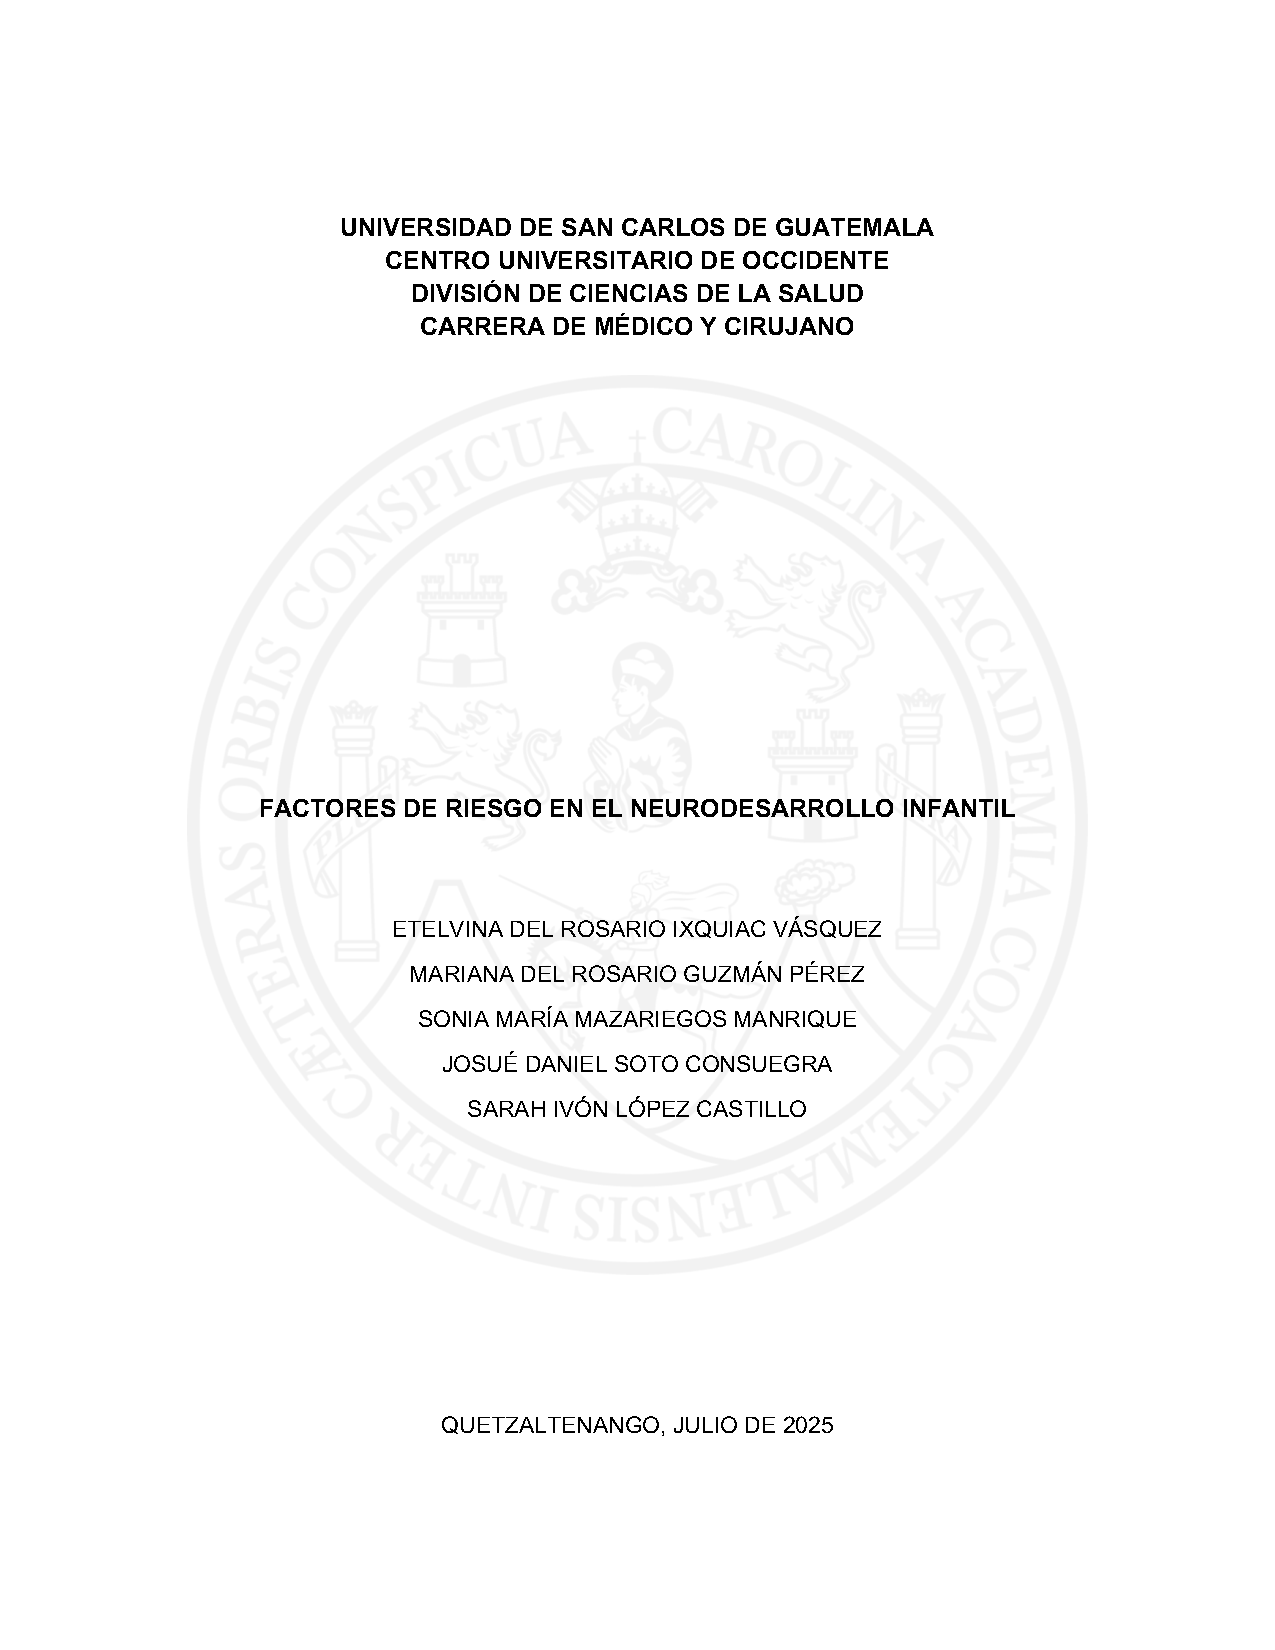
\includepdf[scale=1,pages=-]{extras/caratulas.pdf}
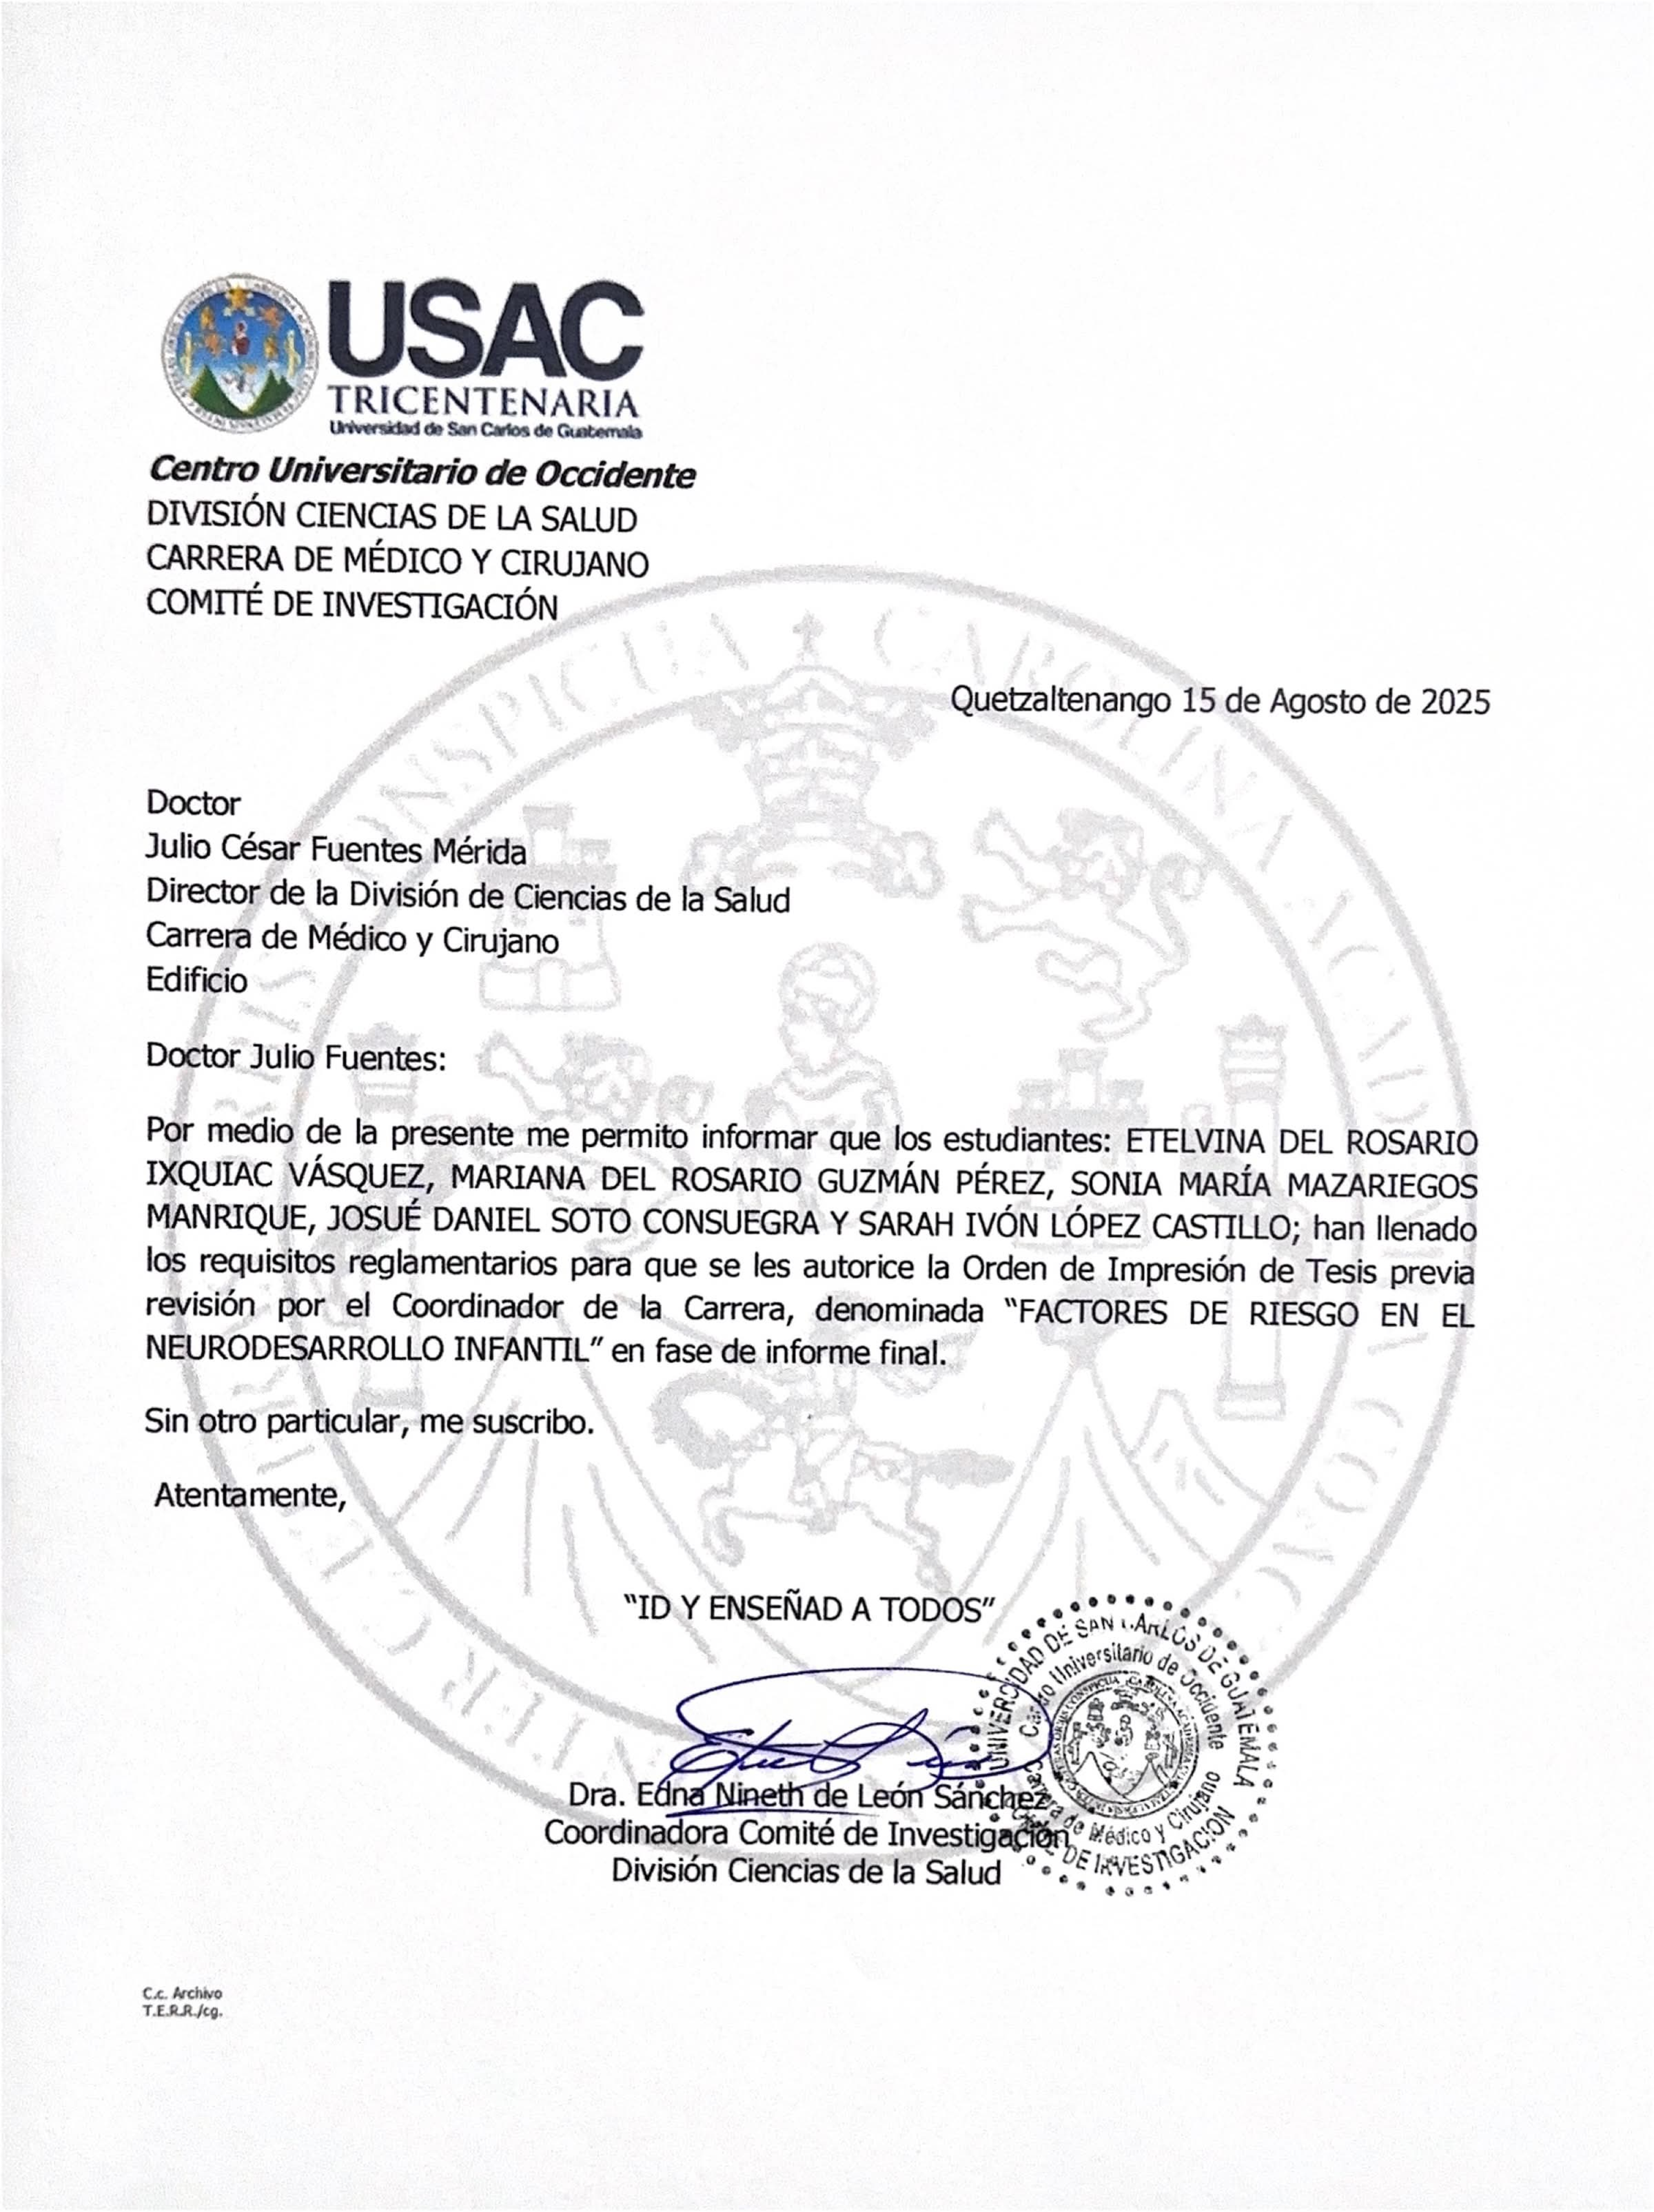
\includepdf[scale=1]{extras/impresion.pdf}
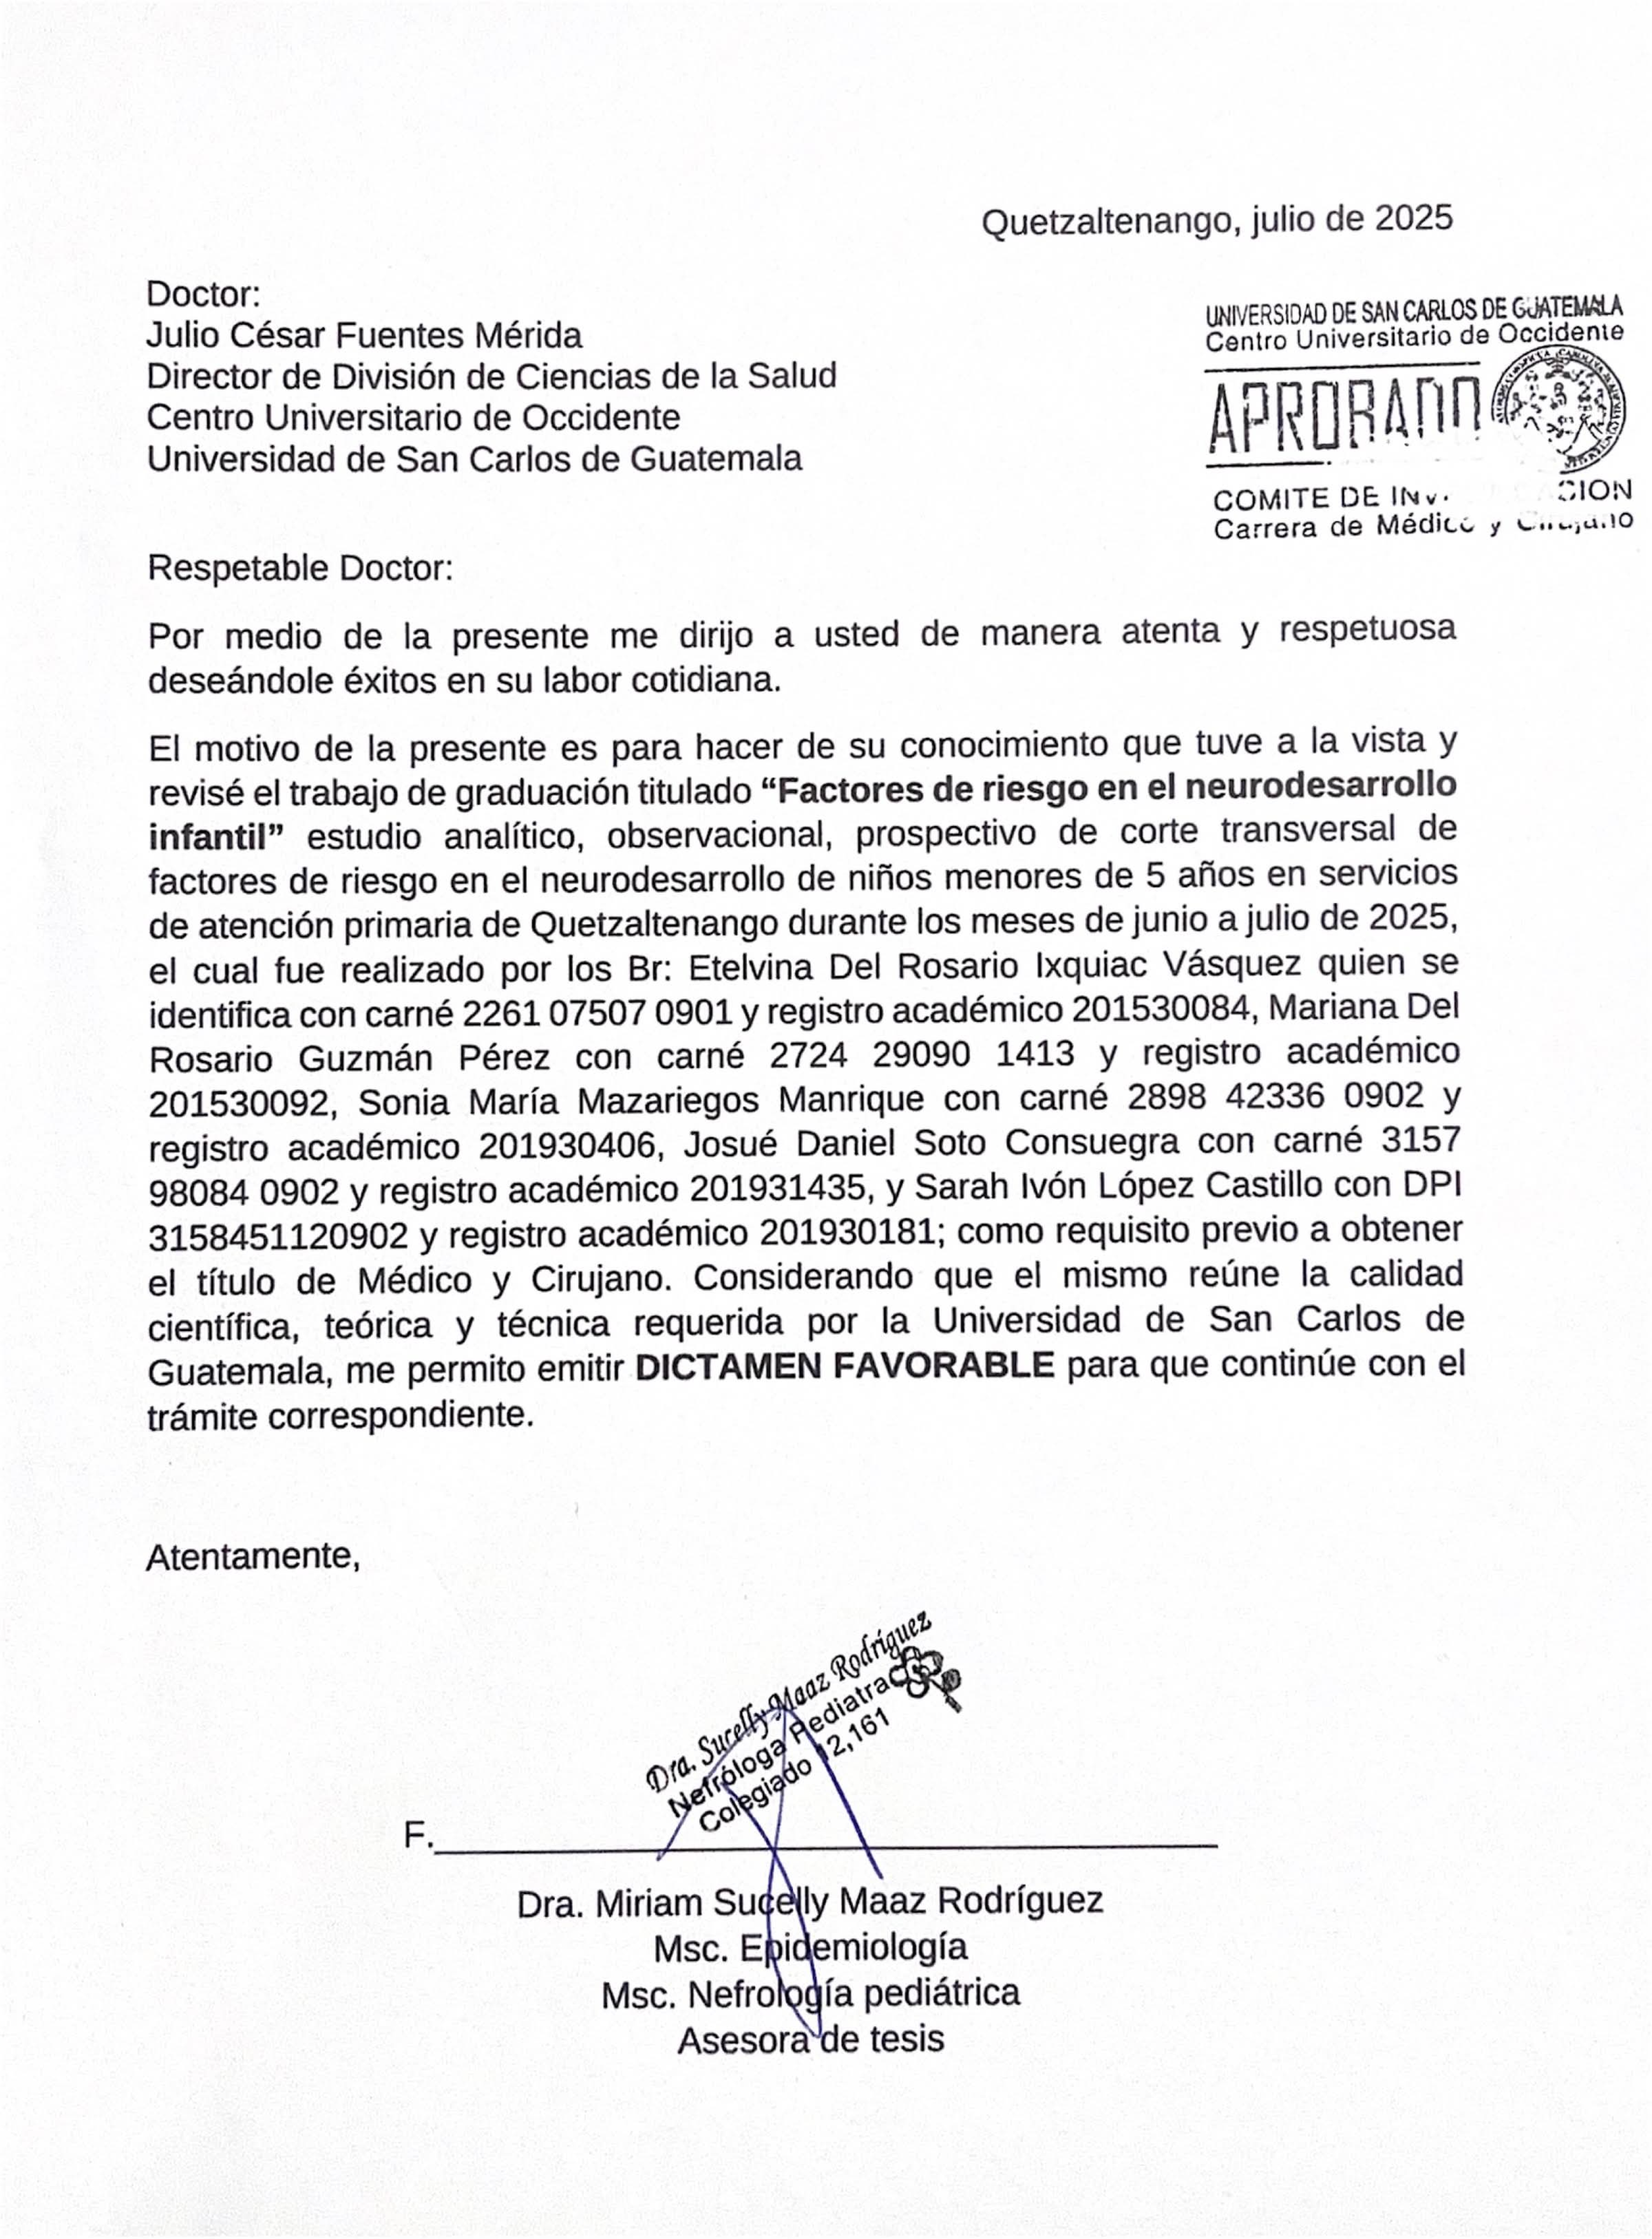
\includepdf[scale=1,pages=-]{extras/dictamen.pdf}
\includepdf[scale=1,pages=2]{extras/dictamen2.pdf}

\chapter*{Dedicatoria}
A mi madre cuyo amor incondicional, sacrificio y  apoyo constante
ha sido el pilar fundamental de mi formación académica y personal. A mi padre
por su paciencia y por enseñarme el valor de la perseverancia. Sus consejos y
apoyo han sido invaluables en cada etapa de este camino.

A mis queridas abuela y bisabuela, cuya memoria y ejemplo de vida continúan
inspirándome y recordándome la importancia del servicio hacia los demás y el
compromiso con la comunidad.

A mis queridos amigos, Sarah, Etelvina, Mariana, Sonia, Ángela, Carlos, Jaime,
Israel, Estuardo, Óscar, Giselle y Gabriela, por siempre estar presentes.

A los doctores Sucelly Maaz, Ricardo Guzmán, Salvador Soto, Priscila González,
quienes participaron en diferentes etapas de esta investigación, muchas gracias
por la motivación y el apoyo para la realización de esta investigación en
beneficio de la niñez guatemalteca.

A Dra. Norma Yxquiac, por su ardua labor en reducir las desigualdades en salud y
su dedicación incansable al servicio de las comunidades más vulnerables de
Guatemala.

A Aaron Swartz y Alexandra Elbakyan, por su esfuerzo en hacer la ciencia
accesible para todos. El conocimiento debe compartirse entre todas 
las personas que lo necesitan, no solo entre aquellas que puedan pagarlo.

A la Universidad de San Carlos de Guatemala y al Instituto Guatemalteco de 
Seguridad Social, por ser parte fundamental de mi formación como profesional. 
Eternas gracias a todos los doctores cuya labor altruista y fuerza de voluntad 
contribuyen incansablemente a mejorar la salud de la población guatemalteca.

Finalmente, esta investigación está dedicada con especial cariño a todos los 
niños de Guatemala. Que este trabajo contribuya a crear intervenciones tempranas 
que les permitan alcanzar su máximo potencial de desarrollo, sin importar su 
origen étnico, condición socioeconómica o lugar de residencia. Ellos son la 
razón por la cual esta investigación cobra sentido y significado.

\vspace{1cm}

\begin{center}
\textit{``On ne voit clairement qu'avec le cœur. \\
L'essentiel est invisible aux yeux.''} \\
\textit{--- Antoine de Saint-Exupéry}
\end{center}

\vspace{1cm}

\begin{flushright}
Josué Daniel Soto Consuegra
\end{flushright}

\chapter*{Dedicatoria}
A DIOS: GRACIAS, GRACIAS DIOS, por sostenerme cuando mis fuerzas claudicaban, 
por abrir caminos donde sólo veía muros y por recordarme que cada tropiezo 
también es aprendizaje. Este logro es testimonio de tu fidelidad incalculable 
en mi vida.

A la vida, gracias por las pruebas que formaron mi carácter y por las alegrías 
que me recordaron por qué vale la pena insistir. Hoy cierro una etapa y abro 
otra con la certeza de que seguiré creciendo, sirviendo y aprendiendo.

A mis padres, gracias por no soltarme la mano en los días largos ni en las 
noches de estudio. Este título también lleva sus nombres.

A mi mami, Angélica Vásquez, eres el modelo de la mujer que aspiro a ser:
valiente, trabajadora, amorosa y firme. Tus abrazos me devolvieron la 
calma, tus palabras me devolvieron la fe y tu ejemplo me enseñó que la 
perseverancia transforma los sueños en metas y las metas en realidad. Quiero 
ser como tú.

A mi papi, Edgar Ixquiac, tus consejos han sido guía en mi camino. 
Gracias por creer en mí, por tu paciencia, por enseñarme a pensar con claridad 
y a decidir con corazón y cabeza. Tus palabras me acompañarán en cada turno y 
en cada consulta.

A mi abuelita, Valen ($\dagger$), querida, aunque ya no estés físicamente, tu
amor sigue vivo en mí. Gracias por tu ternura, por cuidar de mí cuando más
necesitaba atención y cariño, por las oraciones silenciosas, por enseñarme que
la bondad también sana, y sobre todo por enseñarme que la fidelidad de Dios
sostiene la vida, y que creer en Él es suficiente siempre. Este logro te honra.

A Mariana Guzmán, gracias por tu compañía incondicional en un camino 
que no ha sido fácil. Durante el trabajo hospitalario me regalaste tu tiempo, 
tu apoyo y tu cariño sin medida. En los días más pesados fuiste descanso, y 
en los días de logro, celebración. Gracias por estar.

A mis padrinos, Paola Cifuentes y Yubini Mérida, gracias por sus consejos 
oportunos y su apoyo especial en cada etapa. Sus palabras sabias, su guía y 
su fe en mi formación hicieron la diferencia cuando la ruta parecía incierta. 
Los llevo conmigo en este logro y en los que vendrán.

Agradezco profundamente a esta casa de estudios que me abrió sus puertas y me 
permitió encontrar valiosos mentores. En especial, a las doctoras Norma Yxquiac
y Sucelly Maaz, quien con su ejemplo me enseñaron la importancia del servicio.
Su guía ha sido fundamental en mi formación profesional y personal.

%\vspace{2cm}

%\begin{center}
%\textit{``El mejor médico es el que conoce la inutilidad \\
%de la mayor parte de las medicinas.''} \\
%\textit{--- Benjamin Franklin}
%\end{center}

%\vspace{1cm}

\begin{flushright}
Etelvina Del Rosario Ixquiac Vásquez
\end{flushright}

\chapter*{Dedicatoria}
A Dios, quien ha sido mi guía, mi refugio y mi fortaleza en cada paso de este 
camino. Su luz me sostuvo y su mano me levantó, enseñándome que incluso en la 
tormenta se puede hallar paz y que todo sacrificio tiene sentido bajo su 
voluntad. A Él entrego este logro, fruto de su amor infinito y de la gracia 
con la que me ha bendecido.

A mi madre, Jacinta Pérez, quien ha sido y seguirá siendo uno de los cimientos 
más sólidos de mi vida. Gracias a tu amor inquebrantable, a tus sacrificios 
silenciosos y a tu esperanza constante en mí, hoy puedo ver materializado este 
sueño de convertirme en Médico y Cirujano. Con tu ejemplo me enseñaste que la 
perseverancia vence a la adversidad y que los logros verdaderos se construyen 
con esfuerzo y entrega. Cada palabra de aliento y todo tu apoyo han quedado 
grabados en mi corazón. Gracias, mamá, por darme alas para volar y raíces 
para nunca olvidar de dónde vengo.

A mi padre, Andrés Guzmán, mi guía y protector, cuyo esfuerzo, entrega y 
sacrificio también son parte esencial de este logro. Con tu trabajo constante 
y tu ejemplo me mostraste que la verdadera fortaleza está en la disciplina y 
en la voluntad de salir adelante. Este triunfo también es tuyo, porque detrás 
de cada paso que di siempre estuvo tu apoyo incondicional, tu confianza en mí 
y tu amor silencioso. Gracias por enseñarme a ser firme frente a la vida.

Agradezco a Etelvina Vásquez, cuyo apoyo y compañía, tanto en la vida 
hospitalaria como en mi vida cotidiana, fueron fundamentales para no rendirme 
y seguir adelante. Con sus palabras y gestos de aliento me enseñó que las 
metas más grandes no se alcanzan en soledad, y este logro también lleva su 
huella.

Mi gratitud eterna a mi querida abuelita Valen ($\dagger$), quien en vida me
brindó cariño, hogar y compañía en los momentos en los que no tuve a mis padres
cerca durante mi carrera. Aunque ya no está físicamente, su recuerdo permanece
vivo en mi corazón, y sé que desde el cielo celebra conmigo este triunfo.

A mis hermanos, Avidan y Esbin, gracias por estar siempre presentes, 
alentándome y sosteniéndome con su apoyo incondicional.

A la Dra. Norma Yxquiac, quien fue parte fundamental en este camino y cuyo 
apoyo y orientación resultaron esenciales para culminar con éxito este proceso 
de investigación.

Finalmente, extiendo un sincero agradecimiento a mi asesora Dra. Sucelly Maaz, y
mi revisor Dr. Ricardo Guzmán por el apoyo y sabiduría durante el proceso de
mi formación profesional.
%\vspace{2cm}

%\begin{center}
%\textit{``La medicina es una ciencia de incertidumbre \\
%y un arte de probabilidad.''} \\
%\textit{--- William Osler}
%\end{center}

%\vspace{1cm}

\begin{flushright}
Mariana Del Rosario Guzmán Pérez
\end{flushright}

\chapter*{Dedicatoria}
Primeramente, agradezco a Dios por brindarme la sabiduría necesaria para
alcanzar este objetivo, así como por su infinita bondad y amor que me han
acompañado durante todo este camino.

A mi madre, Sonia Manrique, mi pilar fundamental, quien me enseñó que ``no
puedo'' no existe en mi vocabulario. Gracias por formarme como una mujer
perseverante y fuerte, por inculcarme los valores que me han convertido en la 
persona que soy hoy. Tu amor incondicional y tu presencia constante a mi lado, 
sin importar las circunstancias, han sido mi mayor fortaleza.

A mi padre, Mario Mazariegos, por su apoyo y amor incondicional, por creer en 
mí y en mis sueños. Tu confianza ha sido un motor fundamental en mi formación 
académica y personal.

A mi hermano, Estuardo Mazariegos, por ser mi ejemplo de hombre exitoso, padre 
amoroso, esposo dedicado e hijo ejemplar. Tu apoyo constante, aún a pesar de 
la distancia, ha sido invaluable en este proceso.

A mi abuela Martha Rodas y mi tía Karla Manrique, mis segundas madres, por su 
apoyo incondicional y sus consejos siempre positivos y sabios que me han 
guiado en los momentos más importantes de mi vida.

A mi pareja, Eduardo Fuentes, y su familia, por brindarme motivación día con 
día y por su amor incondicional. Su ejemplo de constancia, disciplina y 
perseverancia ha sido una inspiración constante en mi crecimiento personal y 
profesional.

A mis queridos amigos Manuela Alvarado, Sarah López y Daniel Soto, por su 
amistad sincera y genuina. Gracias por acompañarme durante todo este proceso 
con su apoyo y compañía incondicional.

A mis asesores, Sucelly Maaz, Norma Yxquiac, y mi revisor Ricardo Guzmán, por su
valiosa orientación y por la confianza depositada en mí durante la elaboración
de este trabajo de investigación.

Finalmente, a mi alma mater, la gloriosa tricentenaria Universidad de San 
Carlos de Guatemala y al Centro Universitario de Occidente, junto con sus 
distinguidos docentes, por brindarme las herramientas y conocimientos 
necesarios para convertirme en una profesional competitiva, llena de 
expectativas y sueños por cumplir.

A todos ustedes, mi más profundo agradecimiento por ser parte de este logro.

%\vspace{2cm}

%\begin{center}
%\textit{``El éxito no es el final, el fracaso no es fatal: \\
%lo que cuenta es el valor para continuar.''} \\
%\textit{--- Winston Churchill}
%\end{center}

\vspace{1cm}

\begin{flushright}
Sonia María Mazariegos Manrique
\end{flushright}

\chapter*{Dedicatoria}
A Dios, por ser mi guía y fortaleza en cada paso de este camino. Por darme la
vida, la salud, y la sabiduría para afrontar cada reto con fe y esperanza.

A mis padres, Simon López y Alby Castillo de López por su amor incondicional,
por enseñarme el valor del esfuerzo y por estar siempre a mi lado,
impulsándome a seguir adelante sin importar las circunstancias. Este logro
también es suyo.

A mis hermanos Alekza, Cody y Jesse López por su cariño, por compartir
conmigo alegrías y dificultades, y por ser mi apoyo constante cuando más lo
necesitaba.

A mis mejores amigos, Daniel Soto, Alan Batz, Alejandra Hernández, Sonia
Mazariegos y Manuela Lem, por su compañía, por cada palabra de aliento, por
las risas que me devolvieron la calma y por recordarme que no estaba sola en
este proceso.

A mis asesores, Dra. Sucelly Maaz, Dra. Norma Yxquiac, y mi revisor Dr. Ricardo
Guzmán, por su paciencia, orientación y compromiso. Gracias por compartir su
conocimiento.

A mis tutoras de electivo en anestesiología, doctoras Estela Herrera, Alejandra
Borja, Hilda Pérez y Esther Ramírez por su dedicación, paciencia, y vocación
docente que provocaron en mí una admiración por su especialidad, su guía
constante marcaron un antes y un después en mi formación profesional.

A mi abuela Saraí Barrios, por su sabiduría, oraciones y amor eterno y a mi
abuelo Amado Castillo ($\dagger$), su ejemplo de vida y enseñanzas me inspiran a
ser mejor cada día, y quien estaría sumamente orgulloso de mi.

A mis primos D'jalma López, Maxy D'Llachieza, Edgar Camposeco, Meylin de
Camposeco, a mis tíos, Gilmar, Osman y Mayen López por su apoyo, por las
palabras de ánimo y por estar presentes en mi formación personal y académica.

Al Centro Universitario de Occidente, por brindarme la oportunidad de
formarme como profesional y asi permitir alcanzar esta meta.

A todos ustedes, gracias por ser parte fundamental de este logro. Cada uno
dejó una huella imborrable en esta etapa tan importante de mi vida.

\vspace{0.5cm}

\begin{center}
\textit{``La medicina cura las enfermedades, \\
pero solo el amor cura a las personas.''} \\
\textit{--- Patch Adams}
\end{center}

%\vspace{1cm}

\begin{flushright}
Sarah Ivón López Castillo
\end{flushright}

\chapter*{Abstract}
\pagenumbering{roman}
Neurodevelopmental disorders in early childhood represent a global health 
crisis, with approximately 250 million children under 5 years of age at risk 
of not reaching their developmental potential worldwide. In Guatemala, the 
situation is concerning, with only 49.8\% of children aged 24-59 months 
showing adequate development in health, learning, and psychosocial well-being, 
and significant disparities between indigenous and non-indigenous populations. 
However, comprehensive evidence on specific risk factors associated with 
neurodevelopmental outcomes in Guatemala's diverse regional contexts remains 
limited, particularly in Quetzaltenango. Here we show that sociodemographic, 
economic, and environmental factors are significantly associated with 
neurodevelopmental risk patterns in a sample of 1,725 children under 5 years 
of age attending primary health care services in the Quetzaltenango district. 
Using the Ages and Stages Questionnaire-3 (ASQ-3), we found that 66.96\% of 
children had adequate global development, while 33.04\% showed risk in any 
domain and 5.22\% high risk, with gross motor skills showing the greatest 
vulnerability (16.7\% at risk). Indigenous ethnicity was associated with 
increased risk in problem-solving (OR=1.50, 95\% CI: 1.05-2.16) and 
socio-individual development (OR=1.53, 95\% CI: 1.06-2.21), while rural 
residence showed robust associations with risk across four domains, including 
communication (OR=2.09) and problem-solving (OR=2.77). Maternal education 
level was significantly associated with all developmental domains ($p<0.001$), 
chronic growth retardation affected gross motor and socio-individual 
development, and increased screen time exposure was associated with 
developmental risk across all domains. These findings provide evidence-based 
insights for designing targeted interventions that address socioeconomic, 
educational, and nutritional disparities to improve early childhood 
development in Guatemala's most vulnerable populations.

\textbf{Keywords:} Child Development, Neuropsychological Tests, Developmental
Disabilities, Mass Screening, Risk Assessment.

\chapter*{Resumen}

Los trastornos del neurodesarrollo en la primera infancia representan una 
crisis de salud global, con aproximadamente 250 millones de niños menores de 5 
años en riesgo de no alcanzar su potencial de desarrollo a nivel mundial. En 
Guatemala, la situación es preocupante, con solo el 49.8\% de los 
niños de 24-59 meses mostrando un desarrollo adecuado en salud, aprendizaje y 
bienestar psicosocial, y disparidades significativas entre poblaciones 
indígenas y no indígenas. Sin embargo, la evidencia integral sobre los factores 
de riesgo específicos asociados con los resultados del neurodesarrollo en los 
diversos contextos regionales de Guatemala sigue siendo limitada, 
particularmente en Quetzaltenango. Aquí mostramos que los 
factores sociodemográficos, económicos y ambientales están significativamente 
asociados con patrones de riesgo del neurodesarrollo en una muestra de 1,725 
niños menores de 5 años que asisten a servicios de atención primaria en el 
distrito de Quetzaltenango. Utilizando el Cuestionario de Edades y Etapas-3 
(ASQ-3), encontramos que el 66.96\% de los niños tenían un desarrollo global 
adecuado, mientras que el 33.04\% mostraron riesgo en cualquier dominio y el 
5.22\% alto riesgo, con las habilidades motoras gruesas mostrando la mayor 
vulnerabilidad (16.7\% en riesgo). La etnicidad indígena se asoció con mayor 
riesgo en resolución de problemas (OR=1.50, IC 95\%: 1.05-2.16) y desarrollo 
socio-individual (OR=1.53, IC 95\%: 1.06-2.21), mientras que la residencia 
rural mostró asociaciones robustas con riesgo en cuatro dominios, incluyendo 
comunicación (OR=2.09) y resolución de problemas (OR=2.77). El nivel educativo 
materno se asoció significativamente con todos los dominios del desarrollo 
($p<0.001$), el retardo de crecimiento crónico afectó el desarrollo motor 
grueso y socio-individual, y el aumento del tiempo de exposición a pantallas 
se asoció con riesgo de desarrollo en todos los dominios. Estos hallazgos 
proporcionan conocimientos basados en evidencia para diseñar intervenciones 
dirigidas que aborden las disparidades socioeconómicas, educativas, y
nutricionales  para mejorar el desarrollo infantil temprano en las poblaciones
más  vulnerables de Guatemala.

\textbf{Palabras clave:} Desarrollo Infantil, Pruebas Neuropsicológicas, 
Discapacidades del Desarrollo, Tamizaje Masivo, Evaluación de Riesgos.

\tableofcontents

\clearpage
\pagenumbering{arabic}
\setcounter{page}{1}

\chapter{Introducción}
El neurodesarrollo infantil constituye un proceso dinámico y complejo que 
establece las bases fundamentales del futuro cognitivo, emocional y social de 
los individuos. Durante los primeros años de vida, especialmente en los 
primeros 1000 días, las experiencias tempranas y las interacciones con el 
entorno moldean la arquitectura cerebral, determinando habilidades cruciales 
como el lenguaje, la memoria, la motricidad y el control emocional. Los 
trastornos en este ámbito trascienden el impacto individual, generando una 
carga significativa sobre las familias, los sistemas educativos y de salud 
pública.

A nivel mundial, UNICEF reporta que aproximadamente 250 millones de niños
menores  de 5 años están en riesgo de no alcanzar su potencial de desarrollo,
mientras  que cerca de 200 millones presentan retrasos en su desarrollo global
debido a  la desnutrición en la primera infancia \cite{UNICEF2023}. Esta
realidad se  intensifica particularmente en países de ingresos bajos y medios,
donde las  adversidades socioeconómicas, la pobreza y el acceso limitado a
servicios de  salud crean un entorno adverso para el desarrollo infantil óptimo.

Guatemala presenta uno de los panoramas más desafiantes de Latinoamérica en
materia de desarrollo infantil: según el informe de la línea de base 
de la Gran Cruzada Nacional por la Nutrición 2021/2022, únicamente el 49.8\% 
de los niños guatemaltecos entre 24 y 59 meses se encuentran en el camino 
adecuado de desarrollo, salud, aprendizaje y bienestar psicosocial. Esta 
situación se agrava dramáticamente por el limitado acceso a programas de 
primera infancia, evidenciado por el hecho de que solo el 1.9\% de las madres 
de niños entre 2 y 5 años reportaron que sus hijos habían participado en estos 
programas fundamentales \cite{SESAN2022}.

El contexto guatemalteco presenta desafíos extraordinarios que se manifiestan 
en profundas desigualdades estructurales. La desnutrición crónica afecta al 
46.5\% de los niños menores de 5 años, con disparidades significativas entre 
población indígena (58\%) versus no indígena (34.2\%), y entre áreas rurales 
(53\%) versus urbanas (34.6\%) \cite{EnMaternoInfantil}. Estas desigualdades 
se reflejan directamente en los indicadores de desarrollo: mientras que el 
57.9\% de los niños no indígenas muestra un desarrollo adecuado, solo el 45\% 
de los niños indígenas alcanza este nivel, evidenciando las profundas brechas 
que caracterizan al país \cite{SESAN2022}.

En la región de Quetzaltenango, estos desafíos se intensifican debido a la 
particular convergencia de factores sociodemográficos, económicos y 
ambientales que caracterizan esta zona. A pesar de constituir una de las
regiones económicamente más activas del país, persisten importantes desafíos en
términos de equidad en el acceso a oportunidades de desarrollo infantil.

Esta investigación surgió de la necesidad de generar evidencia científica para
comprender los factores de riesgo asociados al neurodesarrollo infantil
en Quetzaltenango. El objetivo principal de esta investigación fue establecer la
asociación entre factores sociodemográficos, económicos, familiares y médicos
con el riesgo en el neurodesarrollo en niños menores de 5 años en servicios de 
atención primaria en el distrito de Quetzaltenango, mediante evaluaciones con
el \asq. Específicamente, se buscó clasificar los resultados
según grupos de edad para detectar patrones específicos de riesgo, se evaluó
la asociación entre diversos factores de riesgo y el neurodesarrollo, y la
relación entre el acceso a servicios de salud y la presencia de riesgo de
retraso en el desarrollo.

Los hallazgos de este estudio revelan datos alarmantes de la realidad en la que
se desarrollan miles de niños en Quetzaltenango, se identificó que 33.04\% de
los niños presentan riesgo en al menos un dominio del desarrollo, que las
categorías de motricidad son las más afectadas en la población. Se identificó
que el bajo nivel educativo materno, la exposición temprana y prolongada a
pantallas, así como desigualdades sociales, están estrechamente relacionadas
con peores desenlaces en el neurodesarrollo infantil.

Los resultados de este estudio constituyen evidencia fundamental para contribuir
al diseño de intervenciones y políticas públicas que puedan mejorar el
desarrollo infantil temprano en Quetzaltenango. Esta investigación trasciende el
ámbito académico; representa un llamado a la acción para mejorar el futuro de la
niñez guatemalteca. Cada niño que no alcanza su potencial de desarrollo
representa una oportunidad perdida, no solo para él y su familia, sino para el
progreso colectivo de nuestra sociedad. Esperamos fervientemente que estos
hallazgos sean los primeros pasos para transformar la realidad del desarrollo
infantil en Guatemala.

	\chapter{Antecedentes}
\section{Antecedentes y contextualización del neurodesarrollo infantil}
\subsection{Panorama global del desarrollo infantil}
A nivel global,  los desafíos asociados con el desarrollo infantil son amplios
y están influenciados por factores socioeconómicos, culturales y ambientales.
Según UNICEF, aproximadamente 250 millones de niños menores de 5 años están en 
riesgo de no alcanzar su potencial de desarrollo debido a factores como la 
desnutrición, la falta de estimulación temprana y el acceso limitado a 
servicios de salud y educación \cite{UNICEF2023}. Estas condiciones adversas 
son particularmente prevalentes en países de ingresos bajos y medios, donde se 
observan altas tasas de desnutrición crónica y pobreza.

La neurociencia del desarrollo ha demostrado que los primeros años de vida, 
especialmente los primeros 1000 días, son críticos para el desarrollo cerebral. 
Durante este período, las experiencias ambientales y las interacciones con los 
cuidadores moldean la arquitectura del cerebro, impactando habilidades como el 
lenguaje, la memoria y el control emocional \cite{Stiles2010}. Las adversidades 
tempranas, como la pobreza y la desnutrición, pueden tener efectos negativos 
duraderos en la plasticidad cerebral, lo que subraya la importancia de 
intervenciones tempranas y programas de estimulación.

Desde una perspectiva ecológica, el desarrollo infantil está influenciado por 
múltiples sistemas que interactúan entre sí, como se describe en el modelo de 
Bronfenbrenner \cite{Bronfenbrenner2005}. Este enfoque destaca la importancia 
de los entornos inmediatos, como la familia y la comunidad, así como de 
factores más amplios, como las políticas públicas y las normas culturales. En
Guatemala, el acceso limitado a programas de primera infancia y los altos
índices de desnutrición crónica limitan significativamente las oportunidades de
desarrollo infantil, especialmente en comunidades rurales. \cite{SESAN2022}

\subsection{Contexto guatemalteco del neurodesarrollo infantil}
Guatemala se caracteriza por ser un país con una rica diversidad cultural,
conformado por diferentes grupos étnicos: Maya, Garífuna, Xinka y Mestizo. 
Aunque la mayoría de la población guatemalteca (54\%) reside en zonas urbanas,
es importante señalar que la población indígena habita predominantemente en
áreas rurales (57\%). \cite{PoliticaInfanciaGuate}

El panorama demográfico de Guatemala presenta importantes desafíos para la
primera infancia. Según datos del censo poblacional de 2018, en el país habitan
aproximadamente 2,3 millones de niñas y niños menores de 6 años, de los cuales
cerca de un millón viven en condiciones de pobreza y 800 mil en situación de
extrema pobreza. \cite{INE} Los departamentos con mayor proporción de población
infantil temprana son Totonicapán (41.7\%), Huehuetenango (41.4\%) y El Quiché
(41.1\%). \cite{UNICEFAtlas} Adicionalmente, el 3.8\% de la población infantil
y adolescente entre 4 y 17 años presenta algún tipo de dificultad visual,
auditiva, física, de concentración, autocuidado o comunicación. \cite{INE}

Si bien Guatemala constituye la economía más grande de América Central en
términos de población (aproximadamente 17.6 millones de habitantes en 2023) y
actividad económica (con un PIB de 104.4 mil millones de dólares
estadounidenses en 2023), este crecimiento económico no se ha traducido en una
reducción significativa de la pobreza. Para 2023, se estimaba que el 55\% de la
población vivía en condiciones de pobreza, mientras que la economía informal
representaba el 49\% del PIB, con un 71.1\% de la población empleada trabajando
en el sector informal. \cite{WorldBankGuate} Es importante destacar que la
pobreza y las experiencias adversas durante la infancia tienen efectos
fisiológicos y epigenéticos a largo plazo en el desarrollo cerebral y la
cognición. \cite{Luby_2015} \cite{Noble_2015}

La situación del desarrollo infantil en Guatemala es preocupante. De acuerdo
con los datos de 2021-2022, Guatemala ha obtenido un 50\% en el Índice de
Desarrollo Infantil Temprano, lo que significa que apenas la mitad de los niños
entre 24 y 59 meses presenta un desarrollo adecuado en salud, aprendizaje y
bienestar psicosocial. Existen disparidades significativas entre diferentes
grupos poblacionales: mientras que el 57.9\% de los niños no indígenas muestra
un desarrollo adecuado, solo el 45\% de los niños indígenas alcanza este nivel.
\cite{SESAN2022} Las diferencias se acentúan aún más cuando se analiza el
índice en función de la riqueza del hogar, observándose una brecha de 23 puntos
porcentuales entre los hogares con mayor y menor riqueza. \cite{UNICEFGuate}

El limitado acceso a oportunidades educativas constituye otro desafío
fundamental. En 2020, la tasa neta de cobertura en el nivel inicial fue de
apenas el 1.1\% a nivel nacional. En ese mismo año, se registraron 597,195
niñas y niños inscritos en educación preprimaria, con una cobertura nacional
del 60.8\%, representando el 13.8\% del total de estudiantes inscritos en
los distintos niveles educativos. \cite{PoliticaInfanciaGuate} Para niños
menores de 4 años, la cobertura educativa es particularmente baja, mientras que
para niños entre 4 y 6 años alcanza el 64.4\%. \cite{MineducEstadistica}

La situación educativa de la niñez con discapacidad representa un desafío
particular para el país. Según la ENDIS 2016, el 76\% de las niñas y niños
entre 5 y 18 años con algún tipo de discapacidad asiste a la escuela,
observándose una marcada diferencia entre el área urbana (90\%) y el área rural
(61\%). Los niños con limitaciones significativas en el funcionamiento físico o
cognitivo tienen menor probabilidad de ser inscritos en establecimientos
educativos. \cite{PoliticaInfanciaGuate}

Al analizar la relación entre desarrollo infantil temprano y estado
nutricional, los resultados son consistentes con estudios previos que
demuestran que los niños con desnutrición crónica tienden a presentar un menor
desarrollo. En la encuesta de línea base de la Cruzada Nacional por la
Nutrición 2021/2022, esta relación se evidencia claramente: el porcentaje de
niños con desarrollo adecuado es mayor entre aquellos que no presentan
desnutrición crónica (55,6\%) en comparación con quienes padecen este tipo de
malnutrición (43,3\%). \cite{SESAN2022}

La desnutrición crónica afecta aproximadamente al 46.5\% de los niños
guatemaltecos menores de 5 años, reflejando profundas desigualdades sociales.
El porcentaje de desnutrición crónica es significativamente mayor en áreas
rurales (53\% frente a 34.6\% en zonas urbanas), en población indígena (58\%
frente a 34.2\% en población no indígena), en hogares donde las madres carecen
de escolaridad (67.0\% frente a 19.1\% en hogares donde la madre tiene
educación superior), en hogares con menor riqueza económica (65.9\% en el
quintil inferior frente a 17.4\% en el quintil superior) y cuando existe un
menor espaciamiento entre embarazos (57.0\% frente a 39.6\% con mayor
espaciamiento). \cite{EnMaternoInfantil}

Las prácticas de alimentación infantil también presentan importantes desafíos.
Solo el 63.1\% de las niñas y niños reciben lactancia materna dentro de la
primera hora de nacidos, el 53.2\% reciben lactancia materna exclusiva entre
los 0 y 6 meses de edad, y la duración promedio de la lactancia materna
exclusiva es de apenas 2.8 meses. En cuanto a la alimentación complementaria,
el 55.7\% de los niños entre 6 y 23 meses que son amamantados reciben cuatro o
más grupos de alimentos, mientras que el 71.2\% de los niños no amamantados en
este mismo rango de edad reciben una frecuencia mínima de comidas.
\cite{EnMaternoInfantil} \cite{PoliticaInfanciaGuate}

Si bien la calidad del vínculo entre cuidadores y niños constituye un factor
fundamental para el desarrollo infantil óptimo, las estadísticas en Guatemala
revelan un patrón preocupante de violencia ejercida por los cuidadores hacia
los niños bajo su responsabilidad. Un estudio realizado a finales de 2019 en 52
comunidades de los departamentos de Sololá, Alta Verapaz, Baja Verapaz,
Chimaltenango, Quetzaltenango y San Marcos reveló que 8 de cada 10 adultos
consideran que en su comunidad la forma más habitual de corregir a los hijos es
mediante castigos físicos como cincho, chicote, vara, golpes o gritos. La mitad
de los adultos piensa que la falta de este tipo de disciplina refleja una
carencia de carácter por parte de los padres. \cite{PoliticaInfanciaGuate}
\cite{UNICEFComportamientosNinez}

\subsection{Estudios previos sobre factores de riesgo en el neurodesarrollo}
En una revisión sistemática y meta-análisis realizada por Wondmagegn et al.
(2024), titulada ``Prevalencia y determinantes del retraso del desarrollo entre
los niños en países de ingresos bajos y medios: una revisión sistemática y un
metanálisis'', se analizaron 21 estudios primarios publicados entre 2010 y
2024, involucrando a un total de 54,067 niños en países de ingresos bajos y
medios. El objetivo principal fue evaluar la prevalencia combinada del retraso
del desarrollo confirmado y sus determinantes entre los niños en estos países.
Los resultados mostraron una prevalencia combinada de retraso del desarrollo
del 18.83\% (IC 95\%: 15.53-22.12\%). En el análisis de subgrupos, se observó
una alta prevalencia de retraso del desarrollo [26.69\% (IC 95\%: 15.78-37.60)]
en estudios realizados en África. Los determinantes significativos del retraso
del desarrollo fueron la educación materna [OR: 3.04; IC 95\% (2.05, 4.52)] y
el bajo peso al nacer [OR: 3.61; IC 95\% (1.72, 7.57)]. Los autores concluyeron
que la prevalencia combinada de retraso del desarrollo en países de ingresos
bajos y medios era alta en comparación con los países de altos ingresos,
especialmente en África, y que el nivel educativo materno y el peso al nacer
estaban significativamente asociados con los retrasos del desarrollo.
\cite{Wondmagegn2024}

En un estudio transversal realizado por Mehner et al. (2019), titulado
``La asociación de la puntuación de riesgo acumulativo con los resultados de
ASQ-3 en una región rural empobrecida de Guatemala'', se evaluó una muestra de
conveniencia de 148 madres con niños de 12 a 52 meses de edad en una zona rural
de Guatemala. El objetivo principal fue desarrollar una puntuación de riesgo
compuesta por factores fácilmente obtenibles para diseñar intervenciones e
identificar a los niños de alto riesgo que más se beneficiarían de estas. Se
utilizaron encuestas de interacción madre-hijo y \asq\ para evaluar el
desarrollo. Los resultados mostraron que el 58\% de los niños tenían
puntuaciones anormales en $\ge$1 dominio del ASQ-3, y el 35\% en $\ge$2
dominios. Se desarrollaron tres puntuaciones de riesgo: Riesgo Demográfico
Materno (DR), Interacción Madre-Hijo (MCI) y Riesgo Combinado (CR). La
probabilidad de tener $\ge$2 dominios con puntuaciones anormales aumentó
significativamente con un puntaje DR creciente (OR, 1.46 [IC 95\%, 1.15-1.86]
p<0.05) y un puntaje CR creciente (OR, 2.08 [IC 95\%, 1.41-3.07], p<0.05). Los
autores concluyeron que un índice de riesgo acumulativo combinado de factores
demográficos e interacciones madre-hijo parece ser una herramienta útil para
predecir qué niños tienen puntuaciones anormales en múltiples dominios del
desarrollo. \cite{CMehner2019}

En el contexto específico de Guatemala, un análisis del informe de la  línea de
base de la Gran Cruzada Nacional por la Nutrición 2021/2022 revela  datos
preocupantes: la cobertura de programas de primera infancia es extremadamente
limitada, con apenas un 1.9\% de niños entre 2 y 5 años que han asistido alguna
vez a estos programas. Más alarmante aún es que solo el 49.8\% de los niños
guatemaltecos entre 24 y 59 meses muestran un desarrollo adecuado  en las
dimensiones de salud, aprendizaje y bienestar psicosocial \cite{SESAN2022}.
Estos datos son consistentes con las observaciones de Mehner et al.
\cite{CMehner2019} en zonas rurales de Guatemala, donde encontraron que el 58\%
de los niños evaluados presentaban puntuaciones anormales en al menos un
dominio del ASQ-3.

\subsection{Brechas en el conocimiento e importancia del estudio actual}
En el distrito de Quetzaltenango, Guatemala, la vulnerabilidad económica, el
acceso limitado a servicios de salud y los factores nutricionales representan
un riesgo significativo para el neurodesarrollo infantil. Al igual que en otros
países de ingresos bajos y medios, las condiciones adversas en esta región
pueden influir negativamente en los hitos del desarrollo infantil temprano.

Esta problemática local se enmarca en un contexto global igualmente 
preocupante. Según UNICEF\cite{UNICEF2023}, aproximadamente 250 millones de 
niños menores de 5 años a nivel mundial están en riesgo de no alcanzar su 
potencial de desarrollo, con cerca de 200 millones afectados por desnutrición 
en la primera infancia. Particularmente relevante para nuestro estudio es que 
más de 2 de cada 5 niños entre 3 y 4 años no reciben la estimulación temprana 
ni el cuidado parental adecuados, factores que Domek et al.\cite{Domek2023} 
identificaron como críticos para el desarrollo del lenguaje y socioemocional. 

La unión de los datos nacionales con los hallazgos globales subraya la 
necesidad de investigaciones específicas en contextos como Quetzaltenango, 
donde factores socioeconómicos, nutricionales y de acceso a servicios de salud 
pueden influir significativamente en los patrones de desarrollo infantil.

\section{Neurodesarrollo: Definición y relevancia}
El neurodesarrollo es un proceso dinámico y continuo que se extiende desde 
las primeras etapas de la vida intrauterina hasta la adultez, abarcando una 
compleja interacción de factores genéticos, epigenéticos, ambientales y 
sociales. Este proceso es fundamental para el establecimiento de las bases 
cognitivas, emocionales, motoras y sociales de los individuos, las cuales 
son esenciales para su aprendizaje, adaptación y productividad a lo largo 
de la vida \cite{Stiles2010, Nelson49}.

El desarrollo cerebral está regulado por una interacción entre la expresión 
genética y las influencias ambientales. Mientras que los genes proporcionan 
el marco básico para el desarrollo de estructuras neuronales, las 
experiencias tempranas y las interacciones sociales desempeñan un papel 
crítico en la modelación de las conexiones sinápticas y en la poda neuronal. 
Como señala Stiles \cite{Stiles2010}, ``tanto la expresión genética como los
estímulos ambientales son esenciales para el desarrollo cerebral normal, y la
alteración de cualquiera de estos factores puede modificar fundamentalmente los
resultados neurales''. Estos mecanismos epigenéticos, como la metilación del
ADN, permiten que el entorno modifique la expresión genética sin alterar la
secuencia del ADN,  impactando así el desarrollo cerebral y la consolidación de
habilidades cognitivas y emocionales \cite{Roth2011, Feldman2}.

En el aspecto biológico, el neurodesarrollo durante los primeros años de vida
representa un período crítico caracterizado por un desarrollo acelerado, 
durante el cual numerosas estructuras neuronales se construyen y organizan 
siguiendo las siete fases fundamentales del desarrollo cerebral: nacimiento 
celular, migración celular, diferenciación celular, maduración celular, 
sinaptogénesis, muerte celular y poda sináptica, y mielinización.
\cite{Kolb7}

El neurodesarrollo abarca diversos dominios neurológicos fundamentales que 
evolucionan siguiendo trayectorias interconectadas: sensorial, motor grueso y
fino, lingüístico, visuo-espacial, intelectual, memoria, cognición social y
función ejecutiva. La maduración de estos dominios sigue una secuencia
relativamente predecible, aunque con  variaciones individuales significativas,
que se manifiesta a través de la  adquisición de habilidades cada vez más
complejas y refinadas. \cite{Nelson49}

\subsection{Relevancia del neurodesarrollo infantil}
El neurodesarrollo infantil tiene repercusiones tanto individuales como
colectivas, siendo un aspecto clave para la salud pública. Las investigaciones
muestran que retrasos en el neurodesarrollo están asociados con una mayor carga
económica y social, debido a la necesidad de intervenciones educativas, médicas
y sociales.

El neurodesarrollo infantil también está intrínsecamente ligado a las 
desigualdades sociales y económicas. Los niños que viven en condiciones de 
pobreza enfrentan una mayor probabilidad de exposición a factores de riesgo, 
como la desnutrición y la falta de estimulación temprana. Estas desigualdades 
no solo limitan el potencial individual, sino que perpetúan el ciclo de pobreza 
entre generaciones. \cite{UNICEF2023}

Las intervenciones tempranas han demostrado ser una estrategia efectiva para 
mitigar los efectos negativos en el neurodesarrollo. Estas intervenciones
incluyen programas de estimulación temprana, atención prenatal y postnatal de
calidad, y políticas públicas que promuevan el acceso a una nutrición adecuada
y a servicios educativos.

\section{Procesos biológicos del desarrollo cerebral}
El cerebro humano evoluciona a partir de un grupo limitado de células
embrionarias hasta convertirse en el sistema orgánico más complejo, todo ello
durante los escasos 280 días que comprende la gestación humana. Lo que 
distingue principalmente el desarrollo fetal humano del de otras especies es 
precisamente el cerebro, con su masiva corteza prefrontal y su extraordinaria 
capacidad para investigar y reflexionar sobre su propia naturaleza y 
funcionamiento. \cite{Polin124}

El proceso de desarrollo cerebral, genéticamente predeterminado, comprende
siete fases claramente definidas que se despliegan a lo largo de un extenso
período evolutivo. \cite{Kolb7}. Las características de estas fases se
sintetizan en el cuadro \ref{tab:fases-desarrollo-cerebral} y se ilustran en la
figura \ref{fig:embriologiacerebral}. 

\begin{table}[htbp]
\caption{Siete fases del desarrollo cerebral}
\label{tab:fases-desarrollo-cerebral}
\resizebox{\textwidth}{!}{%
\begin{tabular}{ll}
\hline
\multicolumn{1}{c}{\textbf{Fase del desarrollo}} & \multicolumn{1}{c}{\textbf{Proceso}} \\ \hline
1. Nacimiento celular & Origen de las neuronas y la glia \\
2. Migración celular & Movimiento de las células a su posición funcional \\
3. Diferenciación celular & Las células precursoras se transforman en un tipo de célula especializada \\
4. Maduración celular & Crecimiento de dendritas y axones \\
5. Sinaptogénesis & Formación de sitios de comunicación de célula a célula \\
6. Muerte celular y poda sináptica & Muerte celular programada y desmantelamiento de circuitos no usados \\
7. Mielinización & Formación de la vaina de mielina que aumenta la velocidad de neurotransmisión \\ \hline \hline
\footnotesize Modificado de: Kolb, B y Whishaw, I y Campbell T. \cite{Kolb7}
\end{tabular}%
}
\end{table}

\subsection{Desarrollo cerebral en el período embrionario}
\subsubsection{Gastrulación: establecimiento de las capas germinales primordiales}
Uno de los primeros pasos cruciales en el desarrollo cerebral ocurre durante la
tercera semana de gestación, cuando la masa celular interna bilaminar,
compuesta por el epiblasto y el hipoblasto, experimenta el proceso de
gastrulación para formar las tres capas germinales embrionarias fundamentales:
endodermo, mesodermo y ectodermo. \cite{Polin124}

Este proceso se inicia con la aparición de la línea primitiva en la superficie
del epiblasto y la definición del polo cefálico, denominado nodo primitivo.
\cite{MooreEmbryo4}

Durante la gastrulación, el epiblasto adquiere la capacidad de migrar hacia la
línea primitiva mediante el proceso de transformación epitelio-mesenquimal. La
disminución de la adhesión celular permite que las células migratorias del
epiblasto se invaginen en la región del nodo y la línea primitiva, deslaminen
y desplacen a las células del hipoblasto para formar el endodermo y el
mesodermo. Las células restantes del epiblasto se diferencian en ectodermo. El
mesodermo dorsal da origen a la notocorda, estructura que posteriormente induce
al ectodermo suprayacente a engrosarse y formar la placa neural, dando lugar al
neuroectodermo. Este momento marca el final de la gastrulación y el inicio de
la neurulación. \cite{Polin124}

La gastrulación también establece visiblemente los ejes primarios del embrión y
del sistema nervioso: lateral, anteroposterior y dorsoventral. Para el día
embrionario 20, las tres capas germinales (endodermo, mesodermo y ectodermo)
están completamente formadas, siendo el ectodermo la capa que dará origen tanto
a la piel como al sistema nervioso central. \cite{Polin124}

\subsubsection{Neurulación: formación del tubo neural}
La neurulación es el proceso mediante el cual se forma el tubo neural a partir
del plegamiento de la placa neural epitelial. En humanos, este proceso ocurre
en dos fases distintas: la neurulación primaria, durante las semanas 3 y 4 de
gestación, que conduce al desarrollo del cerebro y la médula espinal, y la
neurulación secundaria, durante las semanas 5 y 6, con la formación de la
porción inferior de la médula espinal sacra y coccígea. \cite{Polin124}

La placa neural se forma aproximadamente el día embrionario 21 y para el día 22
el surco neural se hace evidente. La fusión del surco neural comienza el día 23
para formar el tubo neural, cerrándose primero la sección central. La porción
rostral del tubo neural, habitada por las primeras células migratorias, se
convertirá en el cerebro, mientras que la porción caudal, que recibe células
migratorias posteriores, formará la médula espinal. Las regiones rostral y
caudal del tubo neural son las últimas en cerrarse. \cite{Gibb2018}

Para satisfacer la demanda de neuronas que poblarán el cerebro, alrededor del
día 25, las células neuroepiteliales (CNE) comienzan a dividirse de manera
simétrica, produciendo dos CNE con cada división, proceso que continúa hasta
aproximadamente el día 42. Poco antes del inicio de la neurogénesis, estas
células pierden sus uniones estrechas, comienzan a expresar genes gliales e
inician su transformación en células gliales radiales. \cite{Stiles2010}

\subsubsection{Formación de vesículas cerebrales primarias y secundarias}
Al finalizar la neurulación, el embrión mide entre 3 y 5 mm de longitud, y para
el final de la octava semana gestacional alcanza entre 27 y 31 mm, un
incremento de diez veces su tamaño. \cite{Stiles2010}

Justo antes del cierre completo del tubo neural, el extremo anterior del tubo
comienza a expandirse formando las tres vesículas cerebrales primarias: el
prosencéfalo (la vesícula más anterior, precursora del cerebro anterior), el
mesencéfalo (vesícula media, precursora de las estructuras del cerebro medio) y
el rombencéfalo (vesícula posterior, que se desarrollará como cerebro
posterior). \cite{Stiles2010}

Estos tres segmentos se subdividen posteriormente y, al final del periodo
embrionario, están presentes las cinco vesículas cerebrales secundarias. El
prosencéfalo se divide en telencéfalo y diencéfalo, mientras que el
rombencéfalo se divide en metencéfalo y mielencéfalo. El mesencéfalo permanece
sin subdividirse. Estas cinco subdivisiones se alinean a lo largo del eje
rostro-caudal del embrión y establecen la organización primaria del sistema
nervioso central. \cite{Stiles2010}

\subsection{Desarrollo cerebral en el período fetal}
Los eventos embrionarios de las primeras seis semanas de desarrollo establecen
el patrón tridimensional del cerebro y la médula espinal, determinando el
destino de las primeras células neurales. Las etapas posteriores del desarrollo
se caracterizan por una proliferación y diferenciación masiva de neuronas y
células gliales, seguidas por la migración y organización de la corteza
cerebral y cerebelosa, el crecimiento dendrítico, la sinaptogénesis y,
finalmente, la formación de vainas de mielina alrededor de las neuronas.
\cite{Polin124}

Durante esta fase del desarrollo cerebral, el cerebro previamente liso adquiere
el patrón de plegamiento con giros y surcos típicamente observados en el
cerebro maduro. Este proceso de desarrollo no consiste en fases temporalmente
separadas, sino en una superposición continua de proliferación, migración y
organización neuronal. \cite{Gibb2018}

\subsubsection{Fase 1 - Nacimiento celular}
Todas las neuronas y células gliales derivan de centros proliferativos
especializados cercanos a la superficie pial: la zona ventricular, la zona
subventricular y, como se ha descrito más recientemente, la zona subventricular
externa. El crecimiento cerebral se caracteriza por la proliferación neuronal
entre las semanas 8 y 15 del desarrollo, y posteriormente por la generación de
glía radial que cambia a una multiplicación principalmente glial a mediados del
segundo trimestre, extendiéndose hasta la vida posnatal. \cite{Polin124} 

El primordio cortical está compuesto por células madre neurales pluripotentes
en división y células progenitoras neurales más restrictivas que colectivamente
forman la zona ventricular. \cite{Polin124}

Derivadas de la zona ventricular, las células de la glía radial mantienen mayor
pluripotencia y son capaces de producir tanto neuronas como células gliales
(astrocitos y oligodendrocitos). Las células gliales radiales son células no
neuronales elongadas que cumplen dos funciones: actúan como andamio guía para
la posterior migración de neuronas y como progenitores neurogénicos y gliales.
\cite{Polin124}

\subsubsection{Fase 2 - Migración celular}
Entre las semanas 12 y 20 de gestación, millones de neuronas postmitóticas se
desplazan desde sus sitios de origen en la zona ventricular y la zona
subventricular hacia la corteza en desarrollo y los núcleos profundos, donde
residirán durante toda la vida, ocupando posiciones específicas para formar la
corteza de seis capas, observable a las 28 semanas de gestación. El momento y
la dirección de estas múltiples migraciones simultáneas están estrictamente
regulados, y los trastornos de este proceso son poco comunes.
\cite{Polin124}

Después de que las células se generan en la zona ventricular o subventricular,
migran de manera radial a lo largo de las células gliales radiales. Las células
que forman las capas más profundas de la corteza cerebral salen primero. 
\cite{Polin124}

\subsubsection{Fase 3 - Diferenciación celular}
El neurodesarrollo se inicia con la proliferación de células neuroepiteliales
que se transforman en diferentes poblaciones de progenitores neurales. Estos
progenitores dan origen a diversos subtipos neuronales que migran hacia
regiones cerebrales específicas, estableciendo las bases estructurales y
funcionales del cerebro en formación. \cite{Lindhout2024}

En la corteza cerebral, los primeros progenitores que aparecen son la glía
radial apical, que continúan expandiéndose y produciendo tipos adicionales de
progenitores amplificadores, como los progenitores intermedios y la glía radial
basal o externa. Este conjunto de progenitores corticales eventualmente da
origen a las neuronas corticales, que posteriormente migran hacia la superficie
exterior y forman las distintas capas de la corteza en un orden de adentro
hacia afuera. \cite{Lindhout2024}

Los progenitores intermedios producen neuronas, mientras que las células de
glía radial dan origen tanto a neuronas de proyección como a astrocitos. A
medida que se forman capas sucesivas del manto cortical, los progenitores se
vuelven más limitados en los tipos celulares que pueden generar.
\cite{Lindhout2024}

Cuando las células madre multipotentes se diferencian primero en células
progenitoras neurales y posteriormente en neuronas, las alteraciones en la
metilación del ADN, las modificaciones de histonas, la accesibilidad de la
cromatina y la composición de variantes de histonas median cambios específicos
en la transcripción génica asociados con cada etapa del desarrollo.
\cite{Lindhout2024}

\subsubsection{Fase 4 - Maduración celular}
Una vez que las neuronas alcanzan su destino final, extienden dendritas y un
axón en un intento de establecer conexiones con otras células y convertirse en
parte integral de una red de comunicación. Las dendritas recopilan información
de otras neuronas, mientras que el axón proporciona un medio para enviar
información a neuronas ubicadas más adelante en la línea de comunicación.
Muchas dendritas se extienden desde una neurona para recibir información de
células en la red, pero un solo axón transmite la información procesada por la
célula. \cite{Gibb2018}

Para establecer contactos apropiados, el axón posee un cono de crecimiento en
su extremo principal. Este cono de crecimiento es guiado mediante el muestreo
de moléculas trópicas producidas localmente que finalmente ayudan al axón a
encontrar su objetivo previsto. Una vez identificado ese objetivo, se forma una
conexión llamada sinapsis, que proporciona el medio para la comunicación célula
a célula. En el contexto de la sinapsis, el axón se considera el terminal
presináptico y la dendrita, el terminal postsináptico. \cite{Gibb2018}

\subsubsection{Fase 5 - Sinaptogénesis}
Los principios básicos de la sinaptogénesis incluyen la formación de las
sinapsis más tempranas en las zonas marginal y de la subplaca, un aumento en el
número de sinapsis en la placa cortical hasta un pico que excede el número
adulto, y un período posterior de eliminación sináptica. En el cerebro, las
sinapsis se observan inicialmente en neuronas de la subplaca y la zona marginal.
\cite{Polin124}

Inicialmente, las dendritas aparecen como procesos gruesos con algunas 
ramificaciones finas. A medida que avanza el desarrollo, aparece un gran número
y variedad de espinas dendríticas. Posteriormente comienza la eliminación
sináptica, y se pierde una gran proporción de sinapsis. \cite{Polin124}

Los factores que estimulan la formación y el desarrollo de sinapsis en el
cerebro en desarrollo incluyen tanto eventos independientes de la actividad
como eventos dependientes de la actividad que ocurren después del desarrollo de
receptores en neuronas diana y la generación de actividad eléctrica.
\cite{Polin124}

\begin{figure}[h]
    \centering
    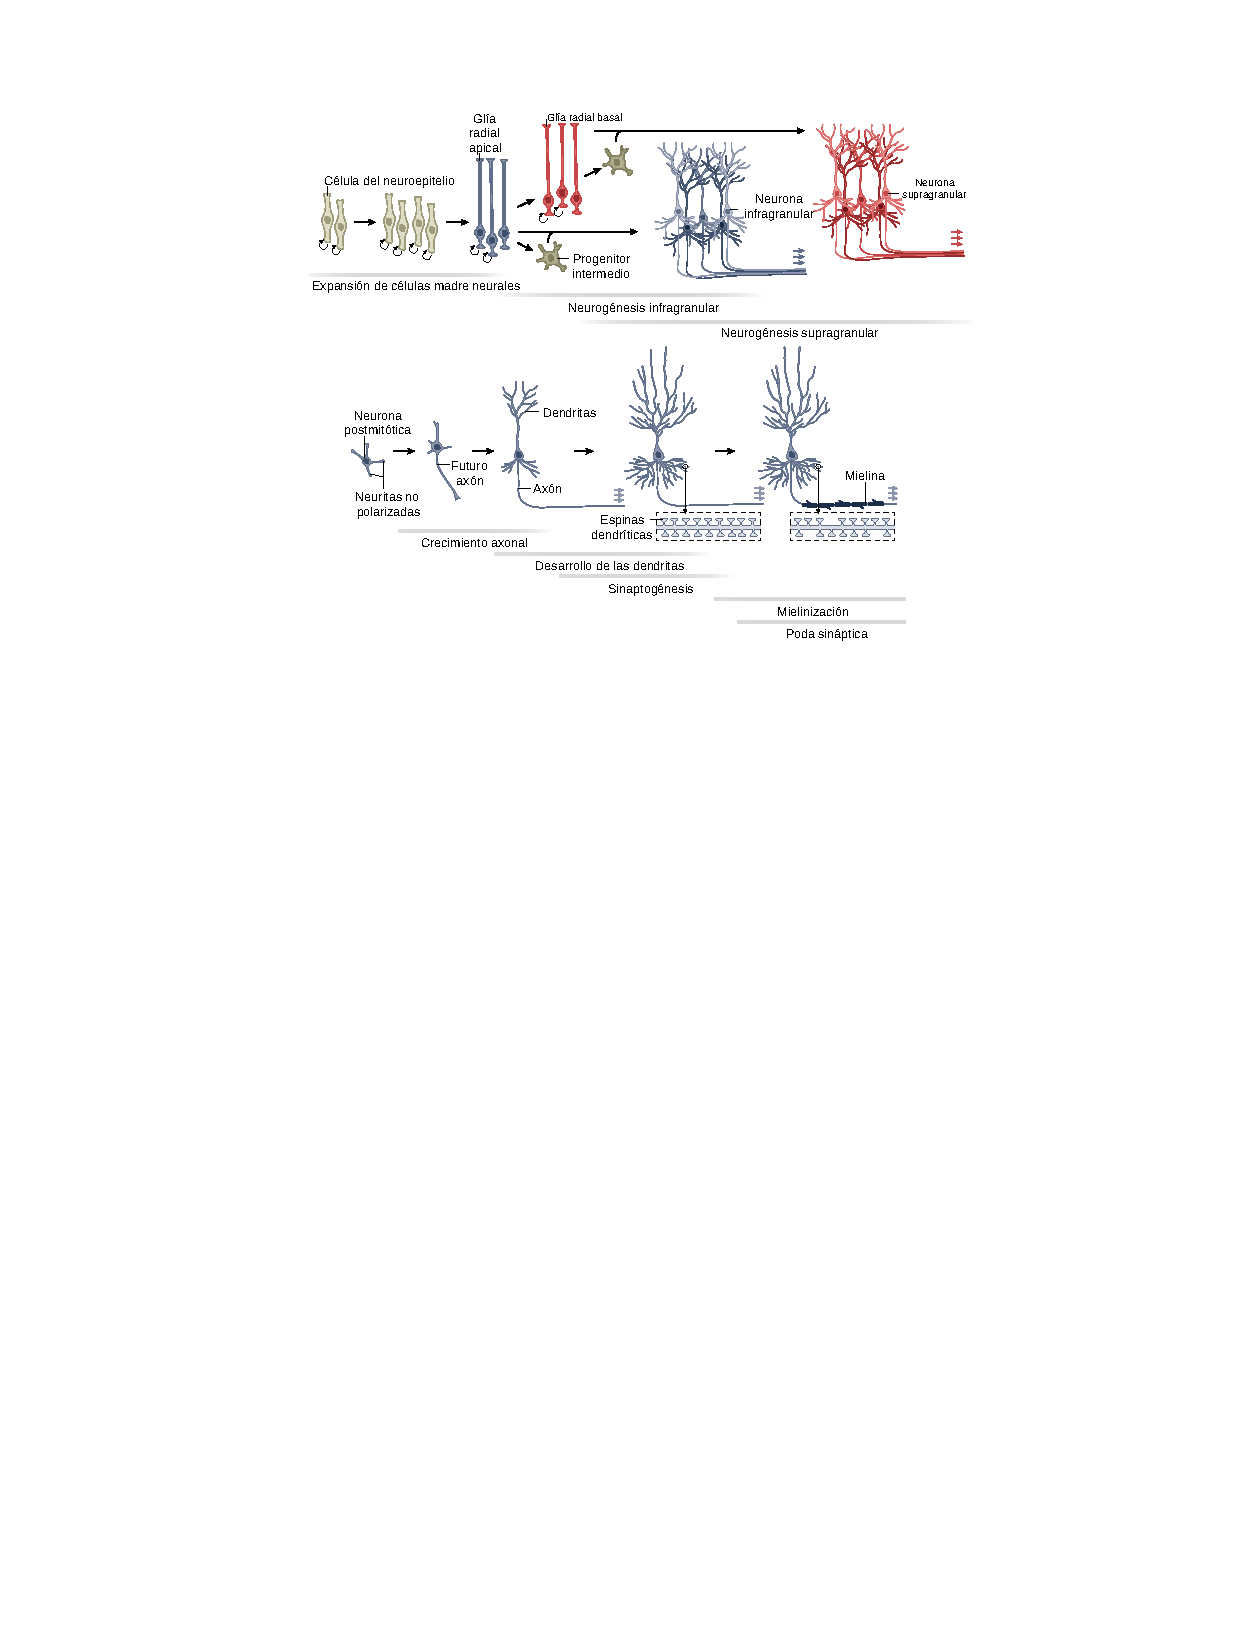
\includegraphics[width=1\textwidth]{embriologiacerebral}
	\captionsetup{font=footnotesize}
    \caption{Procesos biológicos del desarrollo cerebral. Modificado de:
	Lindhout FW, Krienen FM, Pollard KS y Lancaster MA. \cite{Lindhout2024}}
    \label{fig:embriologiacerebral}
\end{figure}

\subsubsection{Fase 6 - Muerte celular y poda sináptica}
La formación del cerebro también depende de procesos degenerativos que
comienzan en el período prenatal. La muerte celular programada o apoptosis se
inicia para reducir el número de células en el cerebro que no han logrado
establecer conexiones útiles o tienen conexiones infrautilizadas.
\cite{Gibb2018}

La muerte celular y la eliminación selectiva de procesos neuronales y sinapsis,
o poda en el desarrollo cerebral, son críticas para el comportamiento posnatal
normal. Típicamente, aproximadamente la mitad de las neuronas en la región
cortical mueren antes de la maduración final. Este proceso de muerte celular
programada, la apoptosis, se inicia y se mantiene por la expresión de genes
específicos. Un aspecto crítico en las fases finales de la secuencia hacia la
muerte celular es la activación de caspasas. \cite{Polin124}

La apoptosis parece ser desencadenada fundamentalmente por la competencia
neuronal por cantidades limitadas de factores tróficos, generados por el
objetivo, la entrada aferente o la glía asociada, permitiendo el emparejamiento
numérico de poblaciones neuronales interconectadas y la eliminación de
proyecciones aberrantes o incorrectas. \cite{Polin124}

\subsection{Desarrollo cerebral en el período postnatal}
Aunque la producción y migración de neuronas son principalmente eventos
prenatales, el desarrollo cerebral continúa de manera significativa después del
nacimiento. La proliferación y migración de progenitores gliales se extiende
durante un período prolongado después del nacimiento, mientras que la
diferenciación y maduración de estas células prosigue a lo largo de toda la
infancia. \cite{Stiles2010}

En el período postnatal, la neurogénesis continúa únicamente en un grado muy
limitado. No obstante, en la zona subventricular, nuevas neuronas siguen
emergiendo y migrando hacia el bulbo olfatorio. Asimismo, se producen neuronas
en el giro dentado del hipocampo, donde migran desde la capa subgranular
solamente hasta la cercana capa granular. Estas formas excepcionales de
neurogénesis parecen continuar durante toda la vida adulta, pero producen solo
un pequeño porcentaje de la población neuronal total.
\cite{Stiles2010}

En contraste con la neurogénesis limitada, la proliferación y migración de
progenitores gliales continúa durante un período prolongado mientras los
oligodendrocitos y astrocitos se diferencian. \cite{Stiles2010}

La sinaptogénesis que comenzó en el período prenatal continúa en el período
postnatal y a lo largo de toda la vida del individuo. La apoptosis continúa
desempeñando un papel fundamental en el desarrollo cerebral durante el período
postnatal. Las sinapsis poco utilizadas son eliminadas en un proceso denominado
poda sináptica, que optimiza los circuitos neuronales para mejorar la
eficiencia funcional. \cite{Gibb2018}

\subsubsection{Fase 7 - Mielinización}
Aunque cierta mielinización ocurre en el período prenatal, este proceso se
intensifica después del nacimiento y continúa hasta bien entrada la tercera
década de vida. El proceso de mielinización predice la maduración de áreas
corticales. Las áreas motoras y sensoriales primarias del cerebro se mielinizan
primero, mientras que las áreas de asociación lo hacen en último lugar.
\cite{Gibb2018}

En el tercer trimestre de gestación, los oligodendrocitos inmaduros desarrollan
extensiones lineales mientras envuelven los axones en preparación para la
mielinización. En el sistema nervioso central, los oligodendrocitos forman
hasta 40 segmentos separados de mielina en múltiples axones, a diferencia del
sistema nervioso periférico, donde las células de Schwann mielinizan axones
individuales. \cite{Polin124}

Los oligodendrocitos maduros se convierten en la etapa oligodendroglial
predominante en los meses posteriores al nacimiento a término y dan origen a la
mielinización. \cite{Polin124}

Después del inicio de la mielinización, los procesos intracelulares comienzan a
intensificarse para crear la composición rica en lípidos de la mielina. El
colesterol, los fosfolípidos y los glucoesfingolípidos representan el 70\% de
la membrana mielínica. Estas células han desarrollado un sistema altamente
eficaz para mantener la proporción óptima de clases de lípidos en la membrana
estrechamente envuelta para realizar su función aislante durante la conducción
nerviosa. \cite{Polin124}

\section{Modelo biopsicosocial del desarrollo infantil}
La biología influye en el comportamiento y el entorno, y a su vez, el
comportamiento y el entorno influyen en la biología a lo largo del desarrollo.
Los niños están influenciados directa e indirectamente tanto por su contexto
cercano como por factores sociales más amplios. El desarrollo infantil es el
producto de la acumulación de interacciones y experiencias cotidianas, así como
del contexto comunitario y cultural más amplio en el que se crían. Si bien los
eventos importantes (como cambios en la estructura familiar) y las
circunstancias (como los recursos familiares) son relevantes para el desarrollo
de los niños, también lo son las interacciones pequeñas que conforman la vida
cotidiana. \cite{Feldman3}

Las influencias tempranas, particularmente aquellas que producen niveles
tóxicos de estrés, afectan al individuo a través de su impacto en los sistemas
de respuesta al estrés del cuerpo, el desarrollo cerebral y la modificación de
la expresión genética. Los cambios epigenéticos, como la metilación del ADN y
la acetilación de histonas, pueden estar influenciados por experiencias
tempranas e impactar la expresión genética sin cambiar la secuencia de ADN.
Estos cambios pueden producir efectos duraderos en la salud y el bienestar del
individuo, y pueden transmitirse a generaciones futuras. \cite{Nelson19}

\subsection{Teorías principales}
Las influencias multinivel y transaccionales en el desarrollo infantil han sido
descritas en dos modelos teóricos fundamentales.

\subsubsection{Teoría de Sistemas Ecológicos de Bronfenbrenner}
La teoría de sistemas ecológicos de Urie Bronfenbrenner propone que existen
múltiples niveles de influencia en el desarrollo infantil, desde las relaciones
con los cuidadores hasta sistemas como las escuelas y lugares de trabajo, hasta
eventos en la sociedad más amplia. El microsistema describe las relaciones e
interacciones directas que tienen los niños, como con cuidadores, hermanos y
compañeros. Estas personas influyen directamente en el niño proporcionando
oportunidades para jugar y aprender, y brindando apoyo emocional. El
microsistema también contiene estructuras con las que el niño interactúa, como
la escuela, el vecindario, entornos de cuidado infantil y la familia. Los niños
tanto influyen como son influenciados por estas relaciones y estructuras.
\cite{Feldman3}

\begin{wrapfigure}{r}[-0.65cm]{0.40\textwidth}
	\centering
    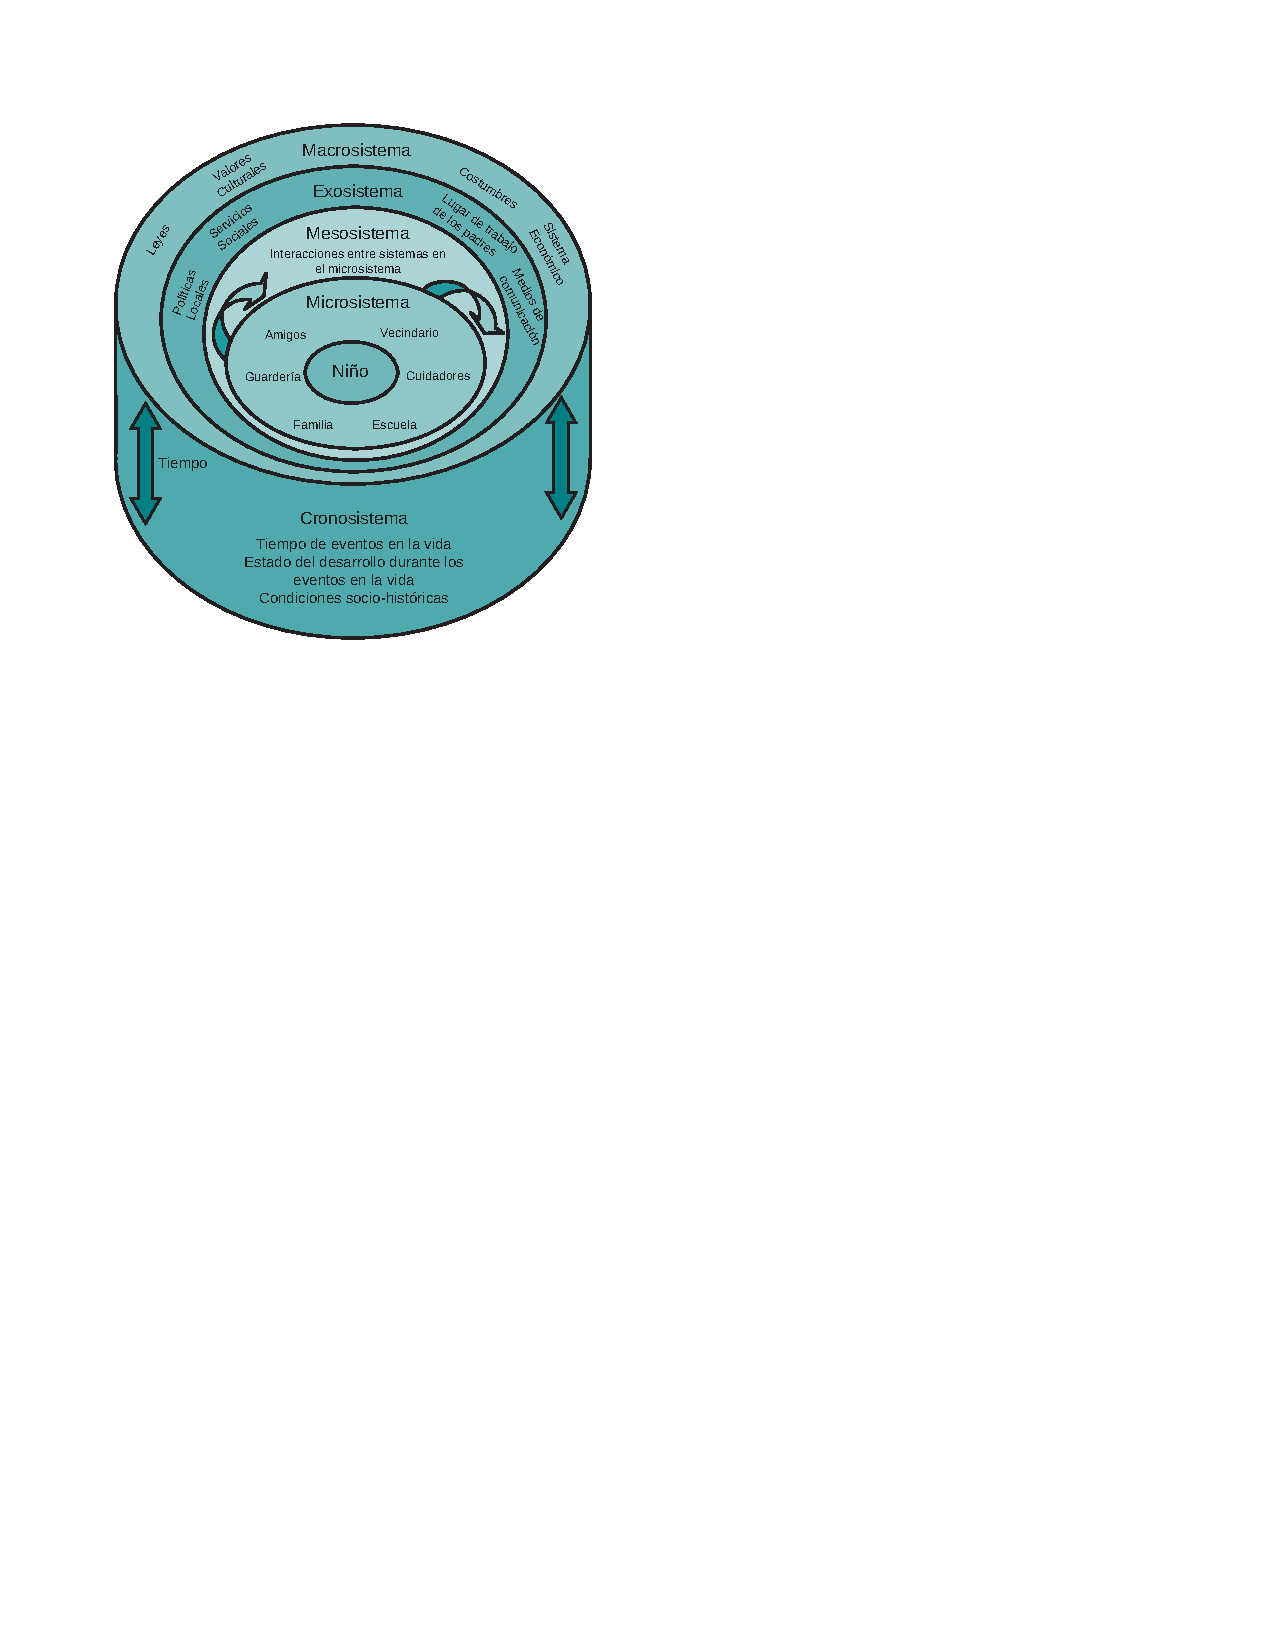
\includegraphics[width=1\linewidth]{sistemasbronfenbrenner}
	\captionsetup{font=footnotesize}
    \caption{La teoría de Bronfenbrenner describe los múltiples niveles que
    impactan al niño en un momento dado y durante el curso del desarrollo.
    Modificado de: Julian M y Lumeng J. \cite{Feldman3}}
    \label{fig:sistemasbronfenbrenner}
\end{wrapfigure}

El mesosistema describe la interacción entre las estructuras que están en el
microsistema. El exosistema consiste en sistemas sociales más grandes que
impactan estructuras en el microsistema. Los niños no interactúan directamente
con el exosistema, pero experimentan el impacto de los cambios en estos sistemas
sociales. El macrosistema es la capa más externa del entorno de un niño y está
definido por valores culturales, costumbres y leyes que influyen en el
funcionamiento de las capas internas. El cronosistema captura la influencia del
tiempo en el desarrollo infantil, reflejando tanto los procesos de desarrollo
que tienen lugar a lo largo del tiempo como la influencia cambiante de los
eventos según su duración y la etapa de desarrollo en la que ocurren.
\cite{Feldman3}

Comprender el ecosistema más amplio del niño es crucial para entender su 
entorno familiar y el contexto de su desarrollo. Factores como la pobreza, el 
racismo, el acceso a la educación, el transporte, los alimentos, la vivienda,
el empleo de los padres y los sistemas de apoyo local influyen
significativamente en el bienestar de un niño. Siempre que sea posible, 
identificar los recursos y activos comunitarios para las familias puede ayudar 
a promover la salud y el desarrollo. \cite{Nelson19}

\subsubsection{Modelo Transaccional de Sameroff}
El modelo transaccional de Arnold Sameroff se basa en las ideas de
Bronfenbrenner sobre la bidireccionalidad de los efectos en el desarrollo
infantil. Discute los procesos que tienen lugar entre padres e hijos en las
interacciones cotidianas y a lo largo del tiempo. Los entornos de los niños
moderan el efecto de los riesgos biológicos tempranos en su desarrollo. La
naturaleza y la crianza se consideran inherentemente inseparables; los genes se
expresan dependiendo del entorno, y los padres responden de manera diferente a
los niños según las características biológicas inherentes del niño.
\cite{Feldman3}

Las características de un niño impactan la crianza, y la crianza impacta el
desarrollo infantil; estas cascadas bidireccionales de influencias continúan a
lo largo del tiempo durante el desarrollo. Es fundamental entender que los
comportamientos de los padres en respuesta a los niños están impulsados por
sus interpretaciones y el significado que extraen del comportamiento. Por
ejemplo, el manejo ansioso de un padre puede surgir debido a su percepción
sobre las complicaciones del nacimiento del niño; un padre puede desvincularse
de un niño con un temperamento difícil debido al significado que atribuye al
comportamiento inquieto del niño. \cite{Sameroff2009}

\subsubsection{Modelo de Diátesis-Estrés}
Este modelo sugiere que algunos individuos son más vulnerables a los impactos
del estrés que otros. Las diátesis o predisposiciones hereditarias o
constitucionales pueden incluir factores biológicos, genéticos, relacionados
con el temperamento o cognitivos que predisponen a un niño a ser vulnerable a
las influencias del estrés. En un entorno favorable para el desarrollo, este
modelo sugiere que tanto los individuos resilientes como los vulnerables
probablemente se desarrollarán bien. En un entorno desafiante, los individuos
resilientes se desarrollarían bien, mientras que los vulnerables no.
\cite{Feldman3}

\subsubsection{Teoría de Susceptibilidad Diferencial}
Esta teoría postula que los individuos varían en su plasticidad, o su nivel de
susceptibilidad a las influencias ambientales. \cite{Belsky2021} Algunos niños,
a veces denominados ``orquídeas'', son muy sensibles a su entorno. Cuando están
en un entorno que apoya ampliamente su desarrollo y bienestar, prosperan; sin
embargo, cuando están en un entorno que no apoya su desarrollo, tienen
dificultades. Otros niños, a veces denominados ``dientes de león'', son menos
susceptibles a las influencias ambientales y se desarrollarán más o menos de la
misma manera independientemente de cuán favorable sea su entorno y sus
relaciones. Los niños pueden ubicarse en cualquier punto del espectro entre
estos dos extremos. \cite{Belsky2021}

\subsection{Relaciones cuidador-niño}
Los cuidadores impactan la biología de un niño a través de sus interacciones con
él. Las interacciones que un niño tiene con el cuidador, o respaldadas por él,
dejan una marca duradera en el genoma del niño y en la estructura cerebral.
A través de la poda neuronal, las conexiones neuronales del niño se refuerzan o
se eliminan según sus experiencias. Los efectos epigenéticos, incluidos los
relacionados con la experiencia del cuidado temprano, también están activos
durante este período de desarrollo. \cite{Roth2011}

La influencia del entorno de crianza domina la mayoría de los modelos actuales
de desarrollo. Los bebés en hospitales y orfanatos, carentes de oportunidades
para el apego, tienen déficits de desarrollo severos. El apego se refiere a
una tendencia determinada biológicamente de un niño pequeño a buscar
proximidad con sus padres durante momentos de estrés y a la relación que
permite a los niños con apego seguro utilizar a sus padres para restablecer una
sensación de bienestar después de una experiencia estresante. El apego inseguro
puede ser predictivo de problemas de comportamiento y aprendizaje posteriores.
\cite{Nelson19}

En todas las etapas del desarrollo, los niños progresan de manera óptima
cuando tienen cuidadores adultos que prestan atención a sus señales verbales y
no verbales y responden en consecuencia. En la primera infancia, esta
capacidad de respuesta contingente a signos de sobreestimulación o baja
estimulación ayuda a mantener a los infantes en un estado de alerta tranquila y
fomenta la autorregulación autonómica. Las respuestas contingentes consistentes
(refuerzo dependiente del comportamiento del otro) a gestos no verbales crean
la base para la atención compartida y la reciprocidad que son críticas para el
desarrollo posterior del lenguaje y social. \cite{Nelson19}

Los cuidadores sirven como guía para el desarrollo cognitivo, social,
conductual, emocional y físico de los infantes. La crianza sensible y receptiva
promueve resultados positivos en los niños en dominios que incluyen el apego,
el desarrollo cognitivo, las habilidades sociales y la regulación emocional.
Un cuidador sensible y receptivo está sintonizado con los sentimientos y
necesidades del niño, y responde con prontitud con acciones que están en
sintonía con los sentimientos y necesidades del niño durante las
actividades cotidianas. \cite{Feldman3}

\subsection{Estrés y trauma infantil}
Incluso a edades tempranas, muchos niños están expuestos a niveles de estrés y
trauma que pueden impactar su desarrollo. El estrés positivo se considera una
parte normal del desarrollo saludable. Las relaciones de cuidado son clave para
amortiguar el efecto de estos factores estresantes, haciendo que los factores
estresantes sean más manejables y que las respuestas biológicas al estrés
disminuyan. El estrés tóxico implica elevaciones del sistema de estrés fuertes,
frecuentes y prolongadas que pueden causar cambios duraderos en los sistemas
neurobiológicos, teniendo un efecto perjudicial en la salud física y mental
posterior. \cite{Feldman3}

Los niños que han experimentado trauma comúnmente presentan comportamiento
agresivo, irritabilidad y retraimiento emocional. Muchos niños volverán a
escenificar el trauma que han experimentado o presenciado, ya sea en vivo o a
través del juego. A menudo, estos factores estresantes ocurren en el contexto
de relaciones de cuidado (ej. abuso o negligencia infantil), lo que magnifica la
experiencia sentida de estrés y disminuye el potencial de amortiguación del
estrés a través de las relaciones. Cuando ocurren en el contexto de relaciones
socioemocionales de apoyo, detección temprana e intervención efectiva, es
probable que estos factores estresantes sean tolerables. \cite{Feldman3}

Los determinantes sociales de la salud son contribuyentes clave a los factores
estresantes y traumas que podrían conducir a elevaciones crónicas en los
sistemas de respuesta al estrés biológico e impactar el desarrollo de los
niños. Las familias que experimentan racismo, discriminación u opresión
económica a menudo experimentan elevaciones crónicas en sus sistemas de
respuesta al estrés biológico que pueden contribuir a una sensación
generalizada de falta de seguridad y protección. Los padres que están
experimentando estos factores estresantes comprensiblemente pueden tener menos
capacidad psicológica para apoyar a sus hijos, ya que es exponencialmente más
difícil ayudar a un niño a sentirse seguro y protegido. \cite{Feldman3}

\section{Teorías del desarrollo y la cognición}
\subsection{Teorías cognitivas}
El desarrollo cognitivo se comprende mejor a través del trabajo de Piaget. Un
principio central del trabajo de Piaget es que la cognición cambia en calidad,
no solo en cantidad. Piaget describió cómo los niños construyen activamente
conocimiento por sí mismos a través de los procesos vinculados de asimilación
(incorporar nuevas experiencias según esquemas existentes) y acomodación (crear
nuevos patrones de comprensión para adaptarse a nueva información). De esta
manera, los niños están continuamente reorganizando activamente los procesos
cognitivos. \cite{Nelson19}

\subsubsection{Jean Piaget: Desarrollo cognitivo}
Jean Piaget (1896-1980) centró su teoría del desarrollo en cómo el niño
desarrolla un marco lógico y científico para comprender el mundo físico.
Postuló que la comprensión de los niños pasa por una serie de cambios
cualitativos o etapas vinculadas a la edad. Cada etapa es un filtro que
selecciona y organiza lo que el niño percibe y entiende. Cada etapa es un marco
que proporciona los componentes básicos para la siguiente, por lo que hay un
orden definido en el que surge la comprensión. El desarrollo ocurre cuando los
niños descubren una discrepancia entre su comprensión actual de la realidad
(asimilación) y las características del mundo que no encajan con esa
comprensión (acomodación). \cite{Feldman3}

Piaget propuso la teoría más conocida del desarrollo cognitivo. En esta teoría,
el desarrollo cognitivo se despliega en cuatro etapas desde la infancia hasta
la adolescencia. Piaget veía el desarrollo cognitivo como una propiedad
inherente a la biología humana, y por lo tanto consideraba las etapas
universales. La suya es una visión constructivista en la que el conocimiento se
desarrolla a través de las actividades de los niños y sus esfuerzos por dar
sentido a sus experiencias. Debido a que el momento de la experiencia puede
variar entre los niños, Piaget asignó edades aproximadas para las etapas.
\cite{Gauvain2022}

Piaget describió dos procesos que regulan el desarrollo cognitivo: organización
y adaptación. La organización se refiere a la estructura secuencial del
desarrollo mental desde un sistema simple a uno más complejo. La adaptación
pertenece a cómo el conocimiento en desarrollo coincide con el entorno, e
incluye dos funciones complementarias. En la asimilación, se añade nueva
información al conocimiento existente, y en la acomodación, se modifica el
conocimiento existente para incluir nueva información. El propósito de la
adaptación es mejorar la alineación entre el pensamiento del individuo y el
entorno, lo que Piaget llamó equilibración. \cite{Gauvain2022}

Con el desarrollo, el pensamiento de los niños cambia desde un enfoque en
experiencias sensoriales y motoras inmediatas y formas simples de entender e
interactuar con el mundo hacia formas más complejas y abstractas de pensar. Las
cuatro etapas se centran principalmente en el razonamiento lógico; son el
período sensoriomotor (0-2 años de edad), preoperacional (2-6 años de edad),
operaciones concretas (6-11 años de edad) y operaciones formales (más de 11
años de edad), estas etapas se resumen en el cuadro \ref{tab:piaget-stages}.
\cite{Gauvain2022}

\begin{table}[htbp]
\caption{Características de las etapas principales en la teoría de Piaget}
\label{tab:piaget-stages}
\fontsize{9}{9}\selectfont
\begin{tabular}{ll}
\hline
Etapa y rango de edad aproximado & Características principales \\ \hline
Sensoriomotor: nacimiento a 2 años & \begin{tabular}[c]{@{}l@{}}La inteligencia está limitada a las propias acciones del infante sobre el\\entorno. La cognición progresa desde el ejercicio de reflejos\\(por ejemplo, succión, orientación visual) hasta el inicio del\\funcionamiento simbólico.\end{tabular} \\
Preoperacional: 2 a 7 años & \begin{tabular}[c]{@{}l@{}}La inteligencia es simbólica, expresada a través del lenguaje, imágenes,\\y otros modos, permitiendo a los niños representar mentalmente y\\comparar objetos fuera de la percepción inmediata. El pensamiento\\es intuitivo en lugar de lógico y es egocéntrico, en el sentido de que\\los niños tienen dificultad para adoptar la perspectiva de otro.\end{tabular} \\
Operaciones concretas: 7 a 11 años & \begin{tabular}[c]{@{}l@{}}La inteligencia es simbólica y lógica, el pensamiento es menos\\egocéntrico. El pensamiento de los niños está limitado a fenómenos\\concretos y sus propias experiencias pasadas; es decir, el pensamiento\\no es abstracto.\end{tabular} \\
Operaciones formales: 11 a 16 años & \begin{tabular}[c]{@{}l@{}}Los niños son capaces de formular y probar hipótesis; la posibilidad\\domina la realidad. Los niños son capaces de reflexionar sobre sus\\propios procesos de pensamiento y, generalmente, pueden pensar\\de manera abstracta.\end{tabular} \\ \hline \hline
\footnotesize Modificado de: Bjorklund \cite{Bjorklund2011-aa}
\end{tabular}
\end{table}

\subsection{Teorías socioculturales}
\subsubsection{Lev Vygotsky: Influencias ambientales en el lenguaje y el pensamiento}
Al igual que Piaget, Lev Vygotsky (1896-1934) estaba interesado en el origen
del conocimiento y de las habilidades de razonamiento, y como Bowlby, estaba
interesado en los efectos de las relaciones humanas en el desarrollo. Desde la
perspectiva de Vygotsky, todos los aspectos del desarrollo humano son el
resultado de interacciones con personas con más experiencia. Esas interacciones
reflejan prácticas culturales. En algunas culturas, se dirige muy poco discurso
hacia los niños pequeños, mientras que en otras culturas se espera que los
niños participen en una conversación. \cite{Feldman3}

El aprendizaje a través de la interacción con otros con mayor experiencia
comienza en la infancia y continúa a lo largo del desarrollo. El otro más
experimentado ayuda a un niño a construir recuerdos, resolver un problema, notar
aspectos del entorno o elaborar sobre la comunicación verbal. \cite{Feldman3}

Otro enfoque importante de la teoría de Vygotsky se refiere al papel del
lenguaje en la formación del pensamiento del niño. Mientras que el pensamiento
y el lenguaje emergen como habilidades humanas independientes, el lenguaje, que
expresa pensamientos, llega a regular primero a través de su expresión externa,
pero más tarde a través de su internalización y expresión en la mente del niño.
\cite{Feldman3}

\subsubsection{Reuven Feuerstein: Mediación social de la cognición}
La teoría y el trabajo aplicado de Reuven Feuerstein (1921-2014) se centran en
la maleabilidad de la cognición e inteligencia de los niños en cada etapa del
desarrollo. Feuerstein teorizó que el desarrollo cognitivo es producto de dos
modalidades de interacción entre el organismo y el entorno. \cite{Feldman3}

Feuerstein distingue entre dos grupos de determinantes del desarrollo cognitivo
diferencial. El primer grupo de determinantes incluye factores genéticos, el
nivel de estimulación ambiental, las relaciones emocionales entre el niño y los
mediadores, y el estatus socioeconómico. En condiciones desfavorables, estos
determinantes interfieren con el desarrollo cognitivo. El segundo grupo de
determinantes consiste en la falta o reducción de exposición a la experiencia
de aprendizaje mediado. \cite{Feldman3}

\subsubsection{Urie Bronfenbrenner: Influencias ambientales directas e indirectas}
Urie Bronfenbrenner (1917-2005) amplió la descripción del entorno que el niño
en crecimiento experimenta tanto directa como indirectamente. Postuló cinco
niveles de influencias ambientales. El más inmediato es el microsistema, que
consiste en entornos sociales que el niño experimenta directamente, como la
familia, los compañeros y la escuela. El microsistema está incrustado en el
mesosistema, el sistema interconectado de microsistemas en los que participa
una persona. El siguiente nivel es el exosistema, que incluye vecinos, medios
sociales y de masas, servicios sociales, industria y política local. Estos
influyen en las personas que influyen en el niño. Más allá está el
macrosistema, las actitudes y creencias de la cultura. Todos estos sistemas
están incrustados en un contexto histórico llamado cronosistema. Estos niveles
del entorno forman una red de conexiones, y el individuo está en su centro
potencialmente influyendo en los niños mientras buscan activamente adaptarse a
su mundo. \cite{Feldman3}

\subsection{Teoría de sistemas dinámicos}
Uno de los enfoques más nuevos para el desarrollo es la teoría de sistemas
dinámicos. Los procesos que pueden explicar el cambio de comportamiento (ej.
potencial genético, procesos neurológicos, características físicas,
estructura familiar, metas y motivos personales) están entrelazados, no son
factores causales independientes. El desarrollo es el resultado de la
interacción de procesos en muchos niveles y muchos sistemas. El desarrollo es
moldeado por fuerzas dentro y fuera de la persona, fusionándose e influyéndose
mutuamente para producir nuevas capacidades y comportamientos. \cite{Newman2020}

El núcleo de la teoría descansa en la definición de sistemas. Todos los
sistemas (biológicos y sociales) están compuestos por elementos
interdependientes que comparten funciones, límites, metas e identidad
interrelacionados. Un sistema dinámico cambia continuamente para llevar a cabo
sus funciones de una manera que mantiene la interacción fluida entre sus
componentes, preservando así el equilibrio. Los elementos se influyen entre sí
y se cambian unos a otros con el tiempo. Entender el desarrollo requiere
considerar eventos momento a momento y su interacción con características
individuales cambiantes. Requiere trazar un camino desde un punto en el tiempo
hasta un punto posterior cuando emerge un comportamiento nuevo y más maduro.
Esto requiere un análisis detallado de múltiples aspectos del comportamiento y
una investigación del proceso de reorganización y crecimiento. La teoría ayuda
a especificar las propiedades de los sistemas que están en flujo (sistemas
abiertos) y cómo la retroalimentación actúa para regular el cambio.
\cite{Feldman3}

La palabra dinámico se utiliza para resaltar la interacción constante y la
influencia mutua de los elementos del sistema. Un componente clave es la
autoorganización, la idea de que el desarrollo se produce a través de las
interacciones de los diversos elementos del sistema. Juntos, estos elementos
producen un conjunto de comportamientos que conducen al cambio cognitivo.
\cite{Gauvain2022}

\section{Trastornos del neurodesarrollo y factores de riesgo}
De acuerdo con el Manual Diagnóstico y Estadístico de los Trastornos Mentales
\cite{DSM5TR}, los trastornos del neurodesarrollo constituyen un grupo de 
afecciones que se manifiestan en las etapas tempranas del desarrollo, 
frecuentemente antes de que el niño ingrese a la escuela, y se caracterizan 
por déficits que producen limitaciones en áreas específicas o globales del
funcionamiento personal, social y académico.

Los trastornos del neurodesarrollo frecuentemente coexisten entre sí; por 
ejemplo, los niños con trastorno del espectro autista a menudo presentan 
trastorno del desarrollo intelectual, y muchos niños con trastorno por déficit
de atención e hiperactividad también presentan algún trastorno específico del
aprendizaje. \cite{DSM5TR}

El DSM-5-TR clasifica los trastornos del neurodesarrollo en seis categorías:
    \begin{itemize}
        \item Trastorno del desarrollo Intelectual
        \item Trastornos de la comunicación
        \item Trastorno del espectro autista
        \item Trastorno por déficit de atención e hiperactividad
        \item Trastorno específico del aprendizaje
        \item Trastornos motores
    \end{itemize}

\subsection{Trastorno del desarrollo intelectual}
\subsubsection{Definición}
El trastorno del desarrollo intelectual se caracteriza por limitaciones 
significativas tanto en el funcionamiento intelectual como en la conducta 
adaptativa, que se manifiestan antes de los 18 años y se expresan en 
habilidades adaptativas conceptuales, sociales y prácticas. \cite{Simms2023}

El funcionamiento adaptativo incluye tres amplios dominios: conceptual, social
y práctico. El dominio conceptual involucra la competencia académica, la
adquisición de conocimientos prácticos y el juicio en situaciones nuevas. El
dominio social implica la conciencia de los pensamientos y sentimientos de los
demás, la empatía, las amistades y el juicio social. El dominio práctico abarca
la capacidad para gestionar los asuntos propios, incluyendo las
responsabilidades escolares y laborales, el manejo del dinero y las
actividades recreativas. \cite{Simms2023}

\subsubsection{Epidemiología}
La prevalencia mundial del trastorno del desarrollo intelectual se estima
entre el 1\% y el 3\%. Se estima que la prevalencia es aproximadamente de 16.4
por cada 1,000 personas en países de bajos ingresos, alrededor de 15.9 por cada
1,000 en países de ingresos medios, y aproximadamente 9.2 por cada 1,000 en
países de altos ingresos. \cite{vanKarnebeek2018, Nelson56}

\subsubsection{Factores de riesgo}
Numerosas causas identificadas del trastorno del desarrollo intelectual pueden
ocurrir antes del nacimiento, durante el parto, después del nacimiento o más 
tarde en la infancia. Estas incluyen infecciones, traumatismos, prematuridad,
hipoxia-isquemia, exposiciones a tóxicos, disfunción metabólica, anomalías
endocrinas, desnutrición y anomalías genéticas. \cite{Nelson56}

Las formas leves y más graves del trastorno presentan factores de riesgo y
etiologías diferentes pero que se sobreponen. Los factores de riesgo no
genéticos frecuentemente asociados con formas leves incluyen bajo nivel
socioeconómico, bajos niveles de educación materna, residencia en un país en
desarrollo, desnutrición y acceso limitado a la atención sanitaria. Las causas
biológicas más comunes o factores de riesgo para las formas leves incluyen
restricción del crecimiento intrauterino, prematuridad, insultos perinatales,
exposición intrauterina a drogas, exposición postnatal a sustancias
neurotóxicas (como el plomo), algunas anomalías cromosómicas sexuales y algunos
síndromes genéticos con múltiples anomalías congénitas mayores o menores.
\cite{Nelson56}

En niños con formas más graves del trastorno, se puede identificar una causa
biológica (generalmente de inicio prenatal) en aproximadamente tres cuartas
partes de los casos. Las causas incluyen trastornos cromosómicos (ej. síndrome
de Down, Wolf-Hirschhorn y deleción 1p36) y otros trastornos genéticos y
epigenéticos (ej. síndromes de X frágil, Rett y Angelman), anomalías del
desarrollo cerebral (ej. lisencefalia), errores innatos del metabolismo y
trastornos mitocondriales (ej. mucopolisacaridosis, trastornos del complejo de
la cadena respiratoria mitocondrial). El trastorno del desarrollo intelectual
grave no sindrómico puede ser resultado de mutaciones genéticas heredadas o de
novo, así como de microdeleciones o microduplicaciones. \cite{Nelson56}

\subsubsection{Diagnóstico}
El diagnóstico formal del trastorno del desarrollo intelectual requiere la
evaluación con pruebas individuales de inteligencia y funcionamiento
adaptativo.

La Escala Bayley de Desarrollo Infantil es la prueba de inteligencia infantil
más utilizada, proporciona una evaluación de las capacidades cognitivas, del
lenguaje, motoras, conductuales, socioemocionales y adaptativas generales para
niños desde los 16 días a los 42 meses de edad. \cite{Nelson56}

Las pruebas de inteligencia más utilizadas para niños mayores de 3 años son las
Escalas Wechsler. Para niños con marcadas limitaciones del lenguaje o verbales,
se pueden emplear pruebas como las Escalas de Habilidades Diferenciales-II o la
Escala Internacional de Rendimiento Leiter, para captar de manera óptima las
habilidades de rendimiento no verbal. \cite{Nelson56}

\subsection{Trastornos de la comunicación}
Los trastornos de la comunicación incluyen déficits en el lenguaje, el habla y
la comunicación. El habla es la producción expresiva de sonidos e incluye la
articulación, fluidez, voz y resonancia de un individuo. El lenguaje abarca la
forma, función y uso de un sistema convencional de símbolos gobernado por reglas
para la comunicación. La comunicación incluye cualquier comportamiento verbal o
no verbal que influye en las ideas, actitudes o comportamientos de otro
individuo. \cite{DSM5TR}

\subsubsection{Trastorno del lenguaje}
Las características esenciales del trastorno del lenguaje son las dificultades
en la adquisición y uso del lenguaje debido a déficits en la comprensión o
producción de vocabulario, gramática, estructura de las oraciones y discurso.
Los déficits del lenguaje son evidentes en la comunicación hablada, escrita o
mediante lenguaje de señas. \cite{DSM5TR}

Los trastornos primarios del desarrollo del habla y lenguaje son dificultades
significativas que se encuentran en ausencia de disfunción cognitiva, sensorial
o motora importante. El criterio para el retraso del lenguaje es un rendimiento
de al menos 1.5 a 2 desviaciones estándar por debajo de la media poblacional en
pruebas estandarizadas de habla o lenguaje. \cite{Feldman44}

Los niños con trastorno del lenguaje pueden tener dificultades significativas
en habilidades lingüísticas de nivel superior, habilidades de razonamiento, la
capacidad para adoptar la perspectiva de otra persona, y la habilidad para
parafrasear y reformular. Algunos niños con este trastorno muestran dificultades
en la interacción social, ya que las interacciones sociales a menudo están
mediadas por el lenguaje verbal. \cite{Nelson53}

\paragraph{Epidemiología}
Los trastornos del lenguaje y del habla son altamente prevalentes.
Aproximadamente el 16\% de los niños muestran retrasos clínicamente
significativos a los 2 años; cerca de la mitad de estos niños continúan
con retrasos hasta el inicio de preprimaria. Los trastornos del lenguaje y habla
pueden ocurrir de forma aislada, juntos o en conjunción con otros retrasos o
trastornos. \cite{Feldman44}

\paragraph{Factores de riesgo}
Los factores genéticos parecen desempeñar un papel importante en cómo los niños
aprenden a hablar. Los antecedentes familiar puede identificar problemas de
habla o lenguaje actuales o pasados en hasta el 30\% de los familiares de
primer grado de niños afectados. La tasa de concordancia para puntuaciones
bajas en pruebas de lenguaje o antecedentes de terapia del habla dentro de
pares de gemelos es aproximadamente del 50\% en pares dicigóticos y del 90\%
en pares monocigóticos. Factores ambientales, hormonales y nutricionales pueden
ejercer influencias epigenéticas al desregular la expresión génica.
\cite{Nelson53}

Los niños criados en orfanatos típicamente experimentan trastornos del
lenguaje y del habla. Los niños que han sufrido abuso y negligencia también
desarrollan frecuentemente trastornos del lenguaje. Para niños que viven en
pobreza, los retrasos en el lenguaje pueden estar relacionados con una pobre
nutrición lingüística y otros desafíos, como mala nutrición y altos niveles
de estrés. \cite{Feldman44}

\paragraph{Diagnóstico}
La evaluación precisa de bebés y niños pequeños es desafiante debido a la
baja frecuencia de producción verbal y la dificultad que tienen los niños
pequeños para cooperar con los clínicos. Las observaciones informales, las
herramientas de entrevista con los padres y las evaluaciones naturales juegan
un papel importante en la evaluación de los niños pequeños. Las evaluaciones
formales se vuelven más relevantes a medida que el niño alcanza la edad
preescolar. \cite{Nelson53}

\paragraph{Comorbilidades}
El trastorno del lenguaje puede asociarse con otros trastornos del
neurodesarrollo en términos de trastorno específico del aprendizaje
(alfabetización y aritmética), trastorno del desarrollo intelectual, trastorno
por déficit de atención e hiperactividad, trastorno del espectro autista y
trastorno de la coordinación del desarrollo. \cite{Feldman44}

\subsubsection{Trastornos de los sonidos del habla}
Un trastorno de los sonidos del habla representa una alteración en la
capacidad para producir los sonidos de las palabras del lenguaje. Un síntoma
primario de la alteración del habla puede ser un discurso ininteligible. Los
trastornos del habla se describen en términos de las características de los
errores de los sonidos del habla o la causa del problema. A menudo no se puede
identificar una causa subyacente para el trastorno de los sonidos del habla.
\cite{Feldman44}

\paragraph{Trastornos de articulación}
La incapacidad para producir correctamente los sonidos del habla se conoce
como trastorno de articulación. Los niños con trastornos de articulación
típicamente muestran errores en un pequeño subconjunto de sonidos
(p. ej., /r, l, s/). En la mayoría de los casos, la causa de un trastorno de
articulación es desconocida; se presume que son resultado de un aprendizaje
incorrecto. Una causa conocida de trastornos de articulación es la pérdida
auditiva bilateral leve a moderada permanente. \cite{Feldman44}

\paragraph{Trastornos fonológicos}
Cuando un niño muestra errores de habla basados en patrones o reglas
implícitas a pesar de la capacidad para producir los mismos sonidos
correctamente en otros contextos, la condición se denomina trastorno
fonológico. Un niño que omite las consonantes finales puede decir ``feli'' en
lugar de ``feliz'' y ``canta'' en lugar de ``cantar'', pero probablemente no
tenga ningún problema al decir palabras como ``zombi'' o ``rana''. El niño está
aplicando una regla incorrecta en lugar de mostrar una incapacidad para
producir el sonido correctamente. \cite{Feldman44}

Los niños con errores fonológicos típicamente tienen déficits moderados a
graves en las habilidades del habla.

\paragraph{Trastornos anatómicos}
La anquiloglosia, o frenillo lingual corto, es una anomalía congénita común
que se ha supuesto que afecta al habla. Sin embargo, la anquiloglosia
típicamente no causa alteraciones del habla. Aunque el frenillo lingual puede
ser significativo al nacer, su gravedad disminuye con el tiempo a medida que
las estructuras orales crecen. Además, los sonidos del habla pueden producirse
con una elevación mínima de la lengua. Cortar el frenillo lingual
típicamente no mejora el habla. Una excepción pueden ser los niños con
parálisis cerebral cuya anquiloglosia está relacionada con alteraciones
neurológicas. \cite{Feldman44}

Los niños con paladar hendido tienen un alto riesgo de presentar trastornos
fonológicos y déficits del lenguaje. Incluso después de la reparación de un
paladar hendido aislado, pueden exhibir patrones de articulación inusuales o
idiosincrásicos. Las estructuras velofaríngeas funcionan anormalmente,
resultando en una incapacidad para generar suficiente presión de aire
intraoral para la producción de consonantes. \cite{Feldman44}

Algunos niños tienen insuficiencia velofaríngea aislada por razones
desconocidas. Estos niños están en riesgo de presentar trastornos de los
sonidos del habla similares a los de los niños con paladar hendido.
\cite{Feldman44}

\paragraph{Trastornos neurológicos}
La disartria es un trastorno del habla asociado con trastornos neuromotores,
como la parálisis cerebral. El tono muscular elevado, la pobre coordinación de
los movimientos motores y la deficiente coordinación de la respiración y la
producción de sonido resultan en movimientos musculares lentos y limitado rango
de movimiento. El habla disártrica tiene una calidad arrastrada y forzada, que
afecta la precisión de la producción de sonidos del habla, la velocidad, el
tono y la entonación. \cite{Feldman44}

La apraxia del habla infantil, conocida anteriormente como apraxia verbal del
desarrollo o dispraxia, es una condición en la que los niños tienen
dificultad con la producción controlada de los sonidos del habla. La etiología
presunta es de origen neurológico, aunque generalmente no se encuentran
lesiones anatómicas. Los niños cometen errores en la producción de vocales y
consonantes y muestran una enorme variabilidad en cómo producen los fonemas y
en el volumen. La inconsistencia en la producción y en los errores hace que la
interpretación de su habla sea muy desafiante. \cite{Feldman44}

\paragraph{Tartamudeo}
El tartamudeo es la causa más común de disfluencia significativa, manifestada
por repetición de sonidos y sílabas y prolongación de vocales o consonantes
realizadas con un flujo de aire continuo. El tartamudeo a menudo se acompaña
de pausas inapropiadas, expresiones faciales repetitivas u otras rutinas
conductuales. Actualmente se considera un trastorno del neurodesarrollo,
caracterizado por el desarrollo atípico de redes neuronales involucradas en la
planificación y ejecución motora del habla. El tartamudeo tiene agregación
familiar, lo que sugiere contribuciones genéticas. \cite{Feldman44}

\subsection{Trastorno del espectro autista}
El trastorno del espectro autista (TEA) representa un grupo de trastornos del
neurodesarrollo que aparecen durante la primera infancia y se caracterizan por
una alteración en la comunicación e interacción social, acompañada de
comportamientos restrictivos y repetitivos.

\subsubsection{Definición del trastorno del espectro autista}
La primera descripción clínica de seis niños con una constelación de rasgos
fácilmente reconocibles como lo que actualmente se conoce como TEA fue
publicada por la psiquiatra rusa Grunya Sukhareva en 1925. \cite{Myers2025}

En 1943, Leo Kanner describió elocuentemente a 11 niños con ``alteraciones
autistas innatas del contacto afectivo'' caracterizadas por un compromiso
social y de interacción profundamente deficiente; alteraciones en la
comunicación que variaban desde el mutismo hasta la ecolalia, inversión
pronominal y literalidad; e interacciones inusuales con el entorno, incluyendo
un ``deseo obsesivo y ansioso por el mantenimiento de la igualdad'' que no se
explicaba por un deterioro cognitivo general. \cite{Myers2025}

Antes del DSM-5, cinco trastornos superpuestos capturaban el espectro:
trastorno autista, trastorno de Asperger, trastorno desintegrativo infantil,
síndrome de Rett y trastorno generalizado del desarrollo no especificado.
\cite{Boland2021-by}

El DSM-5 y la CIE-11 están bien alineados en su conceptualización del TEA como
un diagnóstico único definido por déficits clínicamente significativos y
persistentes en la comunicación e interacción social y comportamientos e
intereses restrictivos y repetitivos atípicos que causan un deterioro
significativo en el funcionamiento adaptativo. Las manifestaciones específicas
de los déficits centrales varían con la edad, la capacidad lingüística e
intelectual, y la gravedad del trastorno. Los síntomas comienzan en el período
de desarrollo pero pueden no manifestarse completamente hasta que las demandas
sociales excedan las capacidades limitadas. Los déficits en la comunicación e
interacción social deben estar presentes en un grado fuera del rango esperado
de funcionamiento para la edad y el nivel de desarrollo intelectual del
individuo. \cite{DSM5TR, Myers2025}

\subsubsection{Epidemiología}
La prevalencia general del TEA en Europa, Asia y Estados Unidos oscila entre 2
y 25 por cada 1000, o aproximadamente 1 de cada 40 a 1 de cada 500. La
prevalencia del TEA ha aumentado con el tiempo, particularmente desde finales
de la década de 1990. Las revisiones sistemáticas de estudios epidemiológicos
sugieren que los cambios en la definición de caso y una mayor percepción del
trastorno explican gran parte del aparente aumento. Existe un predominio
masculino de 4:1. \cite{AutismUpToDate, Nelson58}

\subsubsection{Etiología y Factores de Riesgo}
La patogénesis del TEA no se comprende completamente. El consenso general es
que el TEA es causado por factores genéticos que alteran el desarrollo
cerebral, específicamente la conectividad neuronal, afectando así el
desarrollo de la comunicación social y conduciendo a intereses restrictivos y
comportamientos repetitivos. Este consenso está respaldado por la ``teoría
epigenética'', en la que un gen anormal se ``activa'' al principio del
desarrollo fetal y afecta la expresión de otros genes sin cambiar su secuencia
primaria de ADN. \cite{AutismUpToDate}

Dada la complejidad del TEA y la diversidad de manifestaciones clínicas, es
probable que las interacciones entre múltiples genes o combinaciones de genes
sean responsables del TEA y que factores epigenéticos y la exposición a
modificadores ambientales contribuyan a la expresión variable.
\cite{AutismUpToDate}

Una fuerte contribución genética al desarrollo del TEA está respaldada por la
distribución desigual entre sexos, el aumento de la prevalencia en hermanos,
la alta concordancia en gemelos monocigóticos y el mayor riesgo de TEA con el
aumento del parentesco. \cite{AutismUpToDate}

Los factores prenatales más significativos asociados con el TEA en la
descendencia son la edad materna y paterna avanzada al momento del nacimiento,
sangrado gestacional materno, diabetes gestacional y ser el primer hijo. Los
factores de riesgo perinatales para el TEA incluyen complicaciones del cordón
umbilical, trauma de nacimiento, sufrimiento fetal, pequeño para la edad
gestacional, bajo peso al nacer, baja puntuación de Apgar a los 5 minutos,
malformación congénita, incompatibilidad del sistema de grupos sanguíneos ABO
o factor Rh e hiperbilirrubinemia. \cite{Boland2021-by}

También existe evidencia posible de contribuciones ambientales al TEA. Se han
investigado asociaciones a nivel poblacional con toxinas ambientales como
organofosforados, pesticidas, contaminación del aire y compuestos orgánicos
volátiles. Se considera que un modelo epigenético es una explicación para la
etiología; las personas con vulnerabilidad genética pueden ser más sensibles a
factores ambientales que influyen en el desarrollo cerebral temprano.
\cite{Nelson58}

\subsubsection{Diagnóstico}
Los criterios diagnósticos en el DSM-5 se centran en síntomas en dos dominios 
principales:
    \begin{itemize}
        \item Comunicación e interacción social
        \item Intereses restrictivos y comportamientos repetitivos
    \end{itemize}
Para cumplir con los criterios del TEA, los síntomas deben haber estado
presentes desde el período temprano del desarrollo, afectar significativamente
el funcionamiento y no explicarse mejor por un diagnóstico de discapacidad
intelectual o retraso global del desarrollo. \cite{DSM5TR}

La prueba gold standard es la Escala de Observación para el Diagnóstico del
Autismo (ADOS). \cite{Koth2023}

\subsection{Trastorno por déficit de atención e hiperactividad}
El TDAH es una condición neuropsiquiátrica que afecta a preescolares, niños,
adolescentes y adultos en todo el mundo, caracterizada por falta de atención,
que incluye mayor distractibilidad y dificultad para mantener la atención;
pobre control de impulsos y disminución de la capacidad de autoinhibición; e
hiperactividad motora e inquietud. \cite{Boland2021-by, Nelson50}

El TDAH puede tener su inicio en la infancia, aunque raramente se reconoce
hasta que un niño tiene al menos la edad de un niño pequeño. Más comúnmente,
los bebés con TDAH son activos en la cuna, duermen poco y lloran mucho. Los
niños en edad preescolar con TDAH tienen dificultad para permanecer sentados
durante las actividades en círculo o la hora del cuento y pueden parecer estar
constantemente en movimiento.

Las características más citadas de los niños con TDAH, en orden de frecuencia,
son hiperactividad, déficit de atención (corta duración de la atención,
distractibilidad, perseveración, incapacidad para terminar tareas,
desatención), impulsividad, inquietud, excitabilidad y agresión.
\cite{Boland2021-by}

\subsubsection{Epidemiología}
El TDAH afecta hasta el 5 al 8 por ciento de los niños en edad escolar, con un
60 a 85 por ciento de los diagnosticados como niños que continúan cumpliendo
con los criterios del trastorno en la adolescencia, y hasta un 60 por ciento
que continúa teniendo síntomas significativos en la edad adulta.
\cite{Boland2021-by}

El TDAH es más común en hombres que en mujeres (proporción hombre:mujer 4:1
para la presentación predominantemente hiperactiva-impulsiva y 2:1 para la
presentación predominantemente desatenta). \cite{ADHDUpToDate}

\subsubsection{Etiología y factores de riesgo}
Los datos sugieren que la etiología del TDAH es principalmente genética, con
una heredabilidad de aproximadamente el 75 por ciento. Los síntomas del TDAH
son el producto de interacciones complejas de sistemas neuroanatómicos y
neuroquímicos que sustentan la atención, el control de impulsos y el
funcionamiento ejecutivo. \cite{Boland2021-by}

\subsubsection{Diagnóstico}
La edición actual del DSM-5, publicada en 2013, presenta el diagnóstico del
TDAH como un diagnóstico umbral en el que un niño debe tener al menos seis de
los síntomas descritos de falta de atención o seis de los síntomas descritos
de hiperactividad e impulsividad (al menos cinco para adolescentes mayores de
16 años o adultos), con varios síntomas presentes antes de los 12 años, que
persisten durante al menos 6 meses, ocurren en dos o más entornos y reducen la
calidad del funcionamiento social, académico u ocupacional, mientras que no se
explican mejor por otro trastorno. \cite{Lazar2025}

\subsection{Trastorno específico del aprendizaje}
El trastorno específico del aprendizaje en niños es un trastorno del
neurodesarrollo producido por las interacciones de factores hereditarios y
ambientales que influyen en la capacidad del cerebro para percibir o procesar
información verbal o no verbal de manera eficiente y precisa. Este trastorno
se manifiesta durante los años de educación formal en dificultades
persistentes y limitantes para aprender habilidades académicas fundamentales
como la lectura, la escritura y/o las matemáticas. \cite{Frierson2025}

\subsubsection{Epidemiología}
Se estima que entre el 5\% y el 15\% de los niños en edad escolar luchan
contra un trastorno del desarrollo que interrumpe su educación al afectar su
capacidad para aprender habilidades específicas en los dominios académicos de
lectura, escritura y/o matemáticas. \cite{Frierson2025}

El trastorno específico del aprendizaje varía en gravedad desde leve (p. ej.,
un área única de déficit que afecta solo un dominio académico que puede
requerir una adaptación) hasta severo (p. ej., déficits de aprendizaje que
afectan los tres dominios y que pueden requerir un apoyo extensivo de
educación especial). Las estimaciones reportadas de la proporción entre
hombres y mujeres van desde casi igual (1.15:1) hasta un fuerte predominio
masculino (5:1). El fuerte predominio masculino está particularmente
relacionado con presentaciones más graves del trastorno. \cite{Frierson2025}

\subsubsection{Factores de riesgo}
El trastorno específico del aprendizaje es altamente hereditario. Una persona
con antecedentes familiares de este trastorno tiene cuatro veces más riesgo de
tenerlo. Las causas de estos trastornos son multifactoriales, incluyendo
factores genéticos, madurativos, cognitivos, emocionales, educativos y
socioeconómicos. La prematuridad y el muy bajo peso al nacer también son
factores de riesgo para el trastorno específico del aprendizaje.
\cite{Frierson2025, Boland2021-by}

\subsubsection{Clasificación}
\paragraph{Trastorno específico del aprendizaje con dificultad en la lectura}
La dificultad en la lectura está presente en hasta el 75 por ciento de los
niños y adolescentes con un trastorno específico del aprendizaje. Los
estudiantes que tienen problemas de aprendizaje en otras áreas académicas
comúnmente también experimentan dificultades con la lectura.
\cite{Boland2021-by}

La dificultad en la lectura se caracteriza por problemas en el reconocimiento
de palabras, lectura lenta e imprecisa, pobre comprensión y dificultades con
la ortografía. Esta dificultad a menudo coexiste con otros trastornos en los
niños, particularmente el TDAH. \cite{Boland2021-by}

\paragraph{Trastorno específico del aprendizaje con dificultad en matemáticas}
Los niños con dificultades en matemáticas tienen problemas para aprender y
recordar los números, no pueden recordar hechos básicos sobre los números y son
lentos e imprecisos en los cálculos. Hay cuatro grupos de dificultades
matemáticas: comprensión de hechos, comprensión de procedimientos,
transferencia matemática y memoria para procedimientos matemáticos.

\paragraph{Trastorno específico del aprendizaje con dificultad en la expresión escrita}
La expresión escrita es la habilidad más compleja adquirida para transmitir
una comprensión del lenguaje y expresar pensamientos e ideas. Las habilidades
de escritura están altamente correlacionadas con la lectura para la mayoría de
los niños; sin embargo, algunos niños tienen buenas habilidades de lectura
pero dificultades con la escritura.

Los déficits en la expresión escrita incluyen habilidades de escritura que
están significativamente por debajo del nivel esperado para la edad y
educación de un niño. Tales déficits perjudican el rendimiento académico del
niño y la escritura en las actividades diarias.

\subsection{Trastornos motores}
Los trastornos motores del neurodesarrollo son condiciones que afectan las
habilidades motoras finas y gruesas, generando dificultades en el movimiento,
la coordinación y la ejecución de actividades físicas. Entre los trastornos más
comunes se encuentran los trastornos del desarrollo de la coordinación, los
trastornos de movimientos estereotipados repetitivos y los tics, los cuales
impactan significativamente en el desarrollo y funcionamiento diario de los
niños. \cite{DSM5TR}

El trastorno del desarrollo de la coordinación (TDC) se caracteriza por una
marcada dificultad para adquirir y ejecutar habilidades motoras propias de la
edad, lo que interfiere con actividades cotidianas como vestirse, escribir o
participar en juegos. Estos niños suelen presentar torpeza, movimientos
descoordinados y retrasos en el desarrollo motor, a pesar de no tener un
diagnóstico de condiciones médicas o neurológicas que expliquen estas
dificultades. \cite{DSM5TR}

Por otro lado, los trastornos de movimientos estereotipados repetitivos y los
tics incluyen patrones de movimiento involuntario, repetitivo y rítmico, como
golpear objetos, balancearse o realizar gestos faciales. Los tics pueden ser
motores o vocales, simples o complejos, y suelen fluctuar en intensidad. Estas
condiciones, aunque no siempre interfieren de manera significativa en el
desarrollo, pueden generar desafíos en el ámbito social y emocional,
especialmente si los movimientos son visibles o llaman la atención de los
demás. \cite{DSM5TR}

\section{Tamizaje del neurodesarrollo infantil}
\subsection{Cuestionarios Edades y Etapas 3}
Los ``Cuestionarios Edades y Etapas 3'' (ASQ-3, por sus siglas en inglés) son
una herramienta ampliamente utilizada para la detección temprana de riesgos en
el neurodesarrollo infantil. Diseñados inicialmente en la Universidad de Oregon
en los años 1980, estos cuestionarios han evolucionado hasta convertirse en un
instrumento estandarizado y validado para evaluar múltiples dominios del
desarrollo infantil en niños de 1 mes a 66 meses de vida. Su diseño permite que
sean completados por los padres en colaboración con proveedores de salud, lo
que facilita su implementación en diversos contextos.
\cite{Singh2017, ASQ4decades}

La importancia del ASQ-3 radica en su capacidad para identificar de manera
precisa a niños que podrían beneficiarse de una evaluación más detallada o de
intervenciones tempranas en el desarrollo. Este instrumento evalúa cinco áreas
principales del neurodesarrollo: comunicación, motricidad gruesa, motricidad
fina, resolución de problemas y desarrollo personal-social. Cada cuestionario
consta de 30 ítems específicos para la edad del niño, lo cual asegura
pertinencia y sensibilidad en la evaluación. \cite{squires2009ages}

Desde una perspectiva teórica, el ASQ-3 se alinea con el modelo
biopsicosocial del desarrollo infantil, en el que factores biológicos,
ambientales y sociales interactúan complejamente para influir en los
resultados del desarrollo. Este modelo, descrito por Bronfenbrenner, destaca la
importancia de los entornos inmediatos, como la familia y la comunidad, así
como de factores más amplios, como las políticas públicas y las normas
culturales. En este sentido, el ASQ-3 no solo sirve como una herramienta de
cribado, sino también como un catalizador para intervenciones que
potencialmente pueden transformar los entornos más amplios de los niños
evaluados. \cite{Feldman3, Bronfenbrenner2005}

La validez psicométrica del ASQ-3 ha sido extensivamente documentada reportando
una alta fiabilidad en la evaluación-revaluación (92\%), sensibilidad (87.4\%)
y especificidad (95.7\%). Además, su aplicabilidad ha sido comprobada en
contextos multiculturales y socioeconómicos diversos, incluyendo países de
ingresos bajos y medios, donde su uso requiere adaptaciones contextuales debido
a limitaciones en la alfabetización y el acceso a servicios de salud. En tales
contextos, la evidencia sugiere que los resultados del ASQ-3 son más fiables
cuando los cuestionarios se completan con la orientación de un proveedor de
salud. \cite{Vameghi2013-uo, SarmientoCampos2010, Manasyan2023}

\subsubsection{Contexto histórico de los Cuestionarios Edades y Etapas 3}
El desarrollo de los ``Cuestionarios Edades y Etapas'' inició en 1980 en la
Universidad de Oregon, con la finalidad de evaluar el desarrollo neurológico de
los niños con habilidades que los padres son capaces de reconocer e identificar
en casa. En la década de 1980 a 1990 las doctoras Diane Bricker y Jane Squires
realizaron una búsqueda exhaustiva de conjuntos de habilidades fáciles de ser
elicitadas u observadas por los padres de los niños. En 1995 se publicó una
serie de 8 cuestionarios que evaluaban niños hasta los 48 meses de edad.
\cite{ASQ4decades}

En 1996 se iniciaron estudios de validez, fiabilidad y utilidad de la primera
edición del ``Cuestionario Edades y Etapas''. Para el año 1997 y 1998 se los
estudios determinan las propiedades psicométricas del instrumento de tamizaje.
\cite{ASQ4decades}

En 1999 se publica la segunda edición de los cuestionarios revisados y
extendidos para cubrir hasta la edad de 60 meses. En 2000 se inician
investigaciones a nivel internacional en Finlandia, Noruega, China, Portugal y
Brasil. En 2001 la Academia Americana de Pediatría recomienda el ``Cuestionario
Edades y Etapas'' como una herramienta con buenas propiedades psicométricas,
incluyendo sensibilidad, especificidad, validez y fiabilidad adecuadas, y
estandarizada en diferentes poblaciones. \cite{Pediatrics2001}

Para 2004 se inicia una recolección de datos para la tercera edición del
cuestionario y durante 4 años se recolectan 18,000 cuestionarios de niños de 50
estados de territorios estadounidenses. \cite{ASQ4decades}

Para 2006 la Academia Americana de Pediatría revisa su política de tamizaje del
desarrollo con un algoritmo que incluye cribado a los 9, 18 y 30 meses en
chequeos médicos de rutina y recomienda el ``Cuestionario Edades y Etapas''
como una de las principales herramientas para el tamizaje.
\cite{Pediatrics2006}
 
En 2009 la tercera edición de los cuestionarios es publicada, incluyendo nuevos
valores de estandarización, y puntajes revisados para catalogar a los niños en
áreas de riesgo o de monitoreo. Esta tercera edición se ajusta a los resultados
de 18,000 cuestionarios obtenidos de diferentes contextos socioeconómicos y
lugares en los Estados Unidos de América. \cite{ASQ4decades}

En los Estados Unidos de América es ampliamente utilizada en programas de
chequeo médico de rutina por recomendaciones de la Academia Americana de
Pediatría de realizar por lo menos un tamizaje del desarrollo a las edades de
9, 18 y 30 meses de edad. Otros programas como ``Early Head Start'', ``Help Me
Grow'', ``Child Find'', ``Parents as Teachers'', y programas locales de
condados realizan tamizajes y seguimientos del neurodesarrollo con el
``Cuestionario Edades y Etapas 3'' con mayor frecuencia. \cite{ASQWorld}

\subsubsection{Viabilidad de los Cuestionarios Edades y Etapas 3 en Guatemala}
El uso de los ``Cuestionarios Edades y Etapas 3'' (ASQ-3) en Guatemala presenta
una oportunidad significativa para abordar las disparidades en la detección y
el manejo temprano de problemas del neurodesarrollo infantil. Esta herramienta,
con una fiabilidad de evaluación-reevaluación del 92\%, sensibilidad del 87.4\%
y especificidad del 95.7\%, ha demostrado su robustez psicométrica en diversos
contextos culturales y socioeconómicos, incluyendo países de ingresos bajos y
medios. Sin embargo, la implementación del ASQ-3 en Guatemala requiere
consideraciones específicas dadas las particularidades del sistema de salud y
el entorno sociocultural del país. \cite{Vameghi2013-uo, Manasyan2023}

Una característica clave del ASQ-3 es su enfoque centrado en los padres,
quienes completan los cuestionarios en colaboración con proveedores de salud.
Sin embargo, en contextos como Guatemala, donde la alfabetización funcional y
el acceso a servicios de salud son limitados, la evidencia sugiere que los
resultados son más confiables cuando los cuestionarios se completan con el
apoyo de personal capacitado. Esto resalta la importancia de integrar el ASQ-3
en programas comunitarios y de atención primaria, donde los proveedores de
salud puedan desempeñar un rol clave en la interpretación de resultados y el
seguimiento de casos. \cite{Manasyan2023, Colbert2021}

	\chapter{Objetivos}
\section{Objetivo general}
	\begin{enumerate}
		\item Establecer la asociación entre factores sociodemográficos,
		económicos, familiares y médicos con el riesgo en el neurodesarrollo en
		niños menores de 5 años que asisten a servicios de atención primaria en
		el distrito de Quetzaltenango, mediante evaluaciones con el \asq\
		durante 2025.
	\end{enumerate}
\section{Objetivos específicos}
	\begin{enumerate}
		\item Clasificar los resultados del \asq\ según grupos de edad para
		detectar patrones específicos de riesgo en los dominios del
		neurodesarrollo.
		
		\item Evaluar la asociación entre factores socioeconómicos,
		demográficos, ambientales y antecedentes perinatales y el riesgo de
		retraso en el neurodesarrollo utilizando el \asq.
		
		\item Analizar la relación entre acceso a servicios de atención
		primaria durante el periodo prenatal y postnatal con la presencia de
		riesgo de retraso en el neurodesarrollo.
	\end{enumerate}

	\chapter{Material y método}
\section{Diseño de la investigación}
Estudio de enfoque cuantitativo, diseño analítico, prospectivo
de corte transversal.

\section{Población}
	\begin{enumerate}
		\item Población o universo: Niños menores de 5 años en el área de salud
		del distrito de Quetzaltenango.
		\item Marco muestral: Niños menores de 5 años que acuden a servicios de
		atención primaria en el Puesto de Salud de San José Chiquilajá, Puesto
		de Salud de Pacajá y el Centro de Salud de Quetzaltenango. %\tiempito. 
		\item Muestra: \muestradeseada\ niños menores de 5 años que acudan a
		servicios de atención primaria seleccionados en Quetzaltenango.
	\end{enumerate}

\section{Tamaño de muestra}
El tipo de muestreo fue no probabilístico por conveniencia, se incluyeron a
todos los niños que cumplieron con los criterios de inclusión y asistieron a
servicios de atención primaria, hasta alcanzar el tamaño de muestra deseado
de \muestradeseada\ niños.

\section{Unidad de análisis}
	\begin{enumerate}
		\item Unidad primaria de muestreo: Servicios de atención primaria en
		salud de la ciudad de Quetzaltenango, en específico el Puesto de
		Salud de San José Chiquilajá, Puesto de Salud de Pacajá y el Centro de
		Salud de Quetzaltenango.
		\item Unidad de análisis: Información sobre aspectos sociodemográficos,
		económicos, familiares, perinatales, nutricionales, médicos, de
		interacción y estimulación de los niños y su evaluación de riesgo de
		acuerdo a los dominios del desarrollo de comunicación, área motora
		gruesa y fina, resolución de problemas y área socio-individual.
		\item Unidad de información: Madres o encargados y niños que acudan a
		servicios de atención primaria de la ciudad de Quetzaltenango.
	\end{enumerate}

\section{Hipótesis}
	\begin{enumerate}
		\item Hipótesis nula (H0): No existe una asociación significativa entre
		factores sociodemográficos, condiciones económicas, interacción
		familiar, exposición a dispositivos electrónicos, antecedentes médicos
		perinatales y postnatales, y el riesgo en el neurodesarrollo de niños
		menores de 5 años en servicios de atención primaria de Quetzaltenango.
		\item Hipótesis alternativa (H1): Existe una asociación significativa
		entre factores sociodemográficos, condiciones económicas, interacción
		familiar, exposición a dispositivos electrónicos, antecedentes médicos
		perinatales y postnatales, y el riesgo en el neurodesarrollo de niños
		menores de 5 años en servicios de atención primaria de Quetzaltenango.
	\end{enumerate}

\section{Criterios de inclusión y exclusión}
	\begin{enumerate}
		\item Criterios de inclusión:
			\begin{itemize}
				\item Niños de 0 a 59 meses de edad que acuden a servicios de
				atención primaria para controles de crecimiento y desarrollo,
				vacunación o consulta médica.
				\item Padres o cuidadores que acepten participar en el estudio
				y firmen el consentimiento informado.
			\end{itemize}
		\item Criterios de exclusión:
			\begin{itemize}
				\item Niños con diagnóstico previo de trastornos del
				neurodesarrollo o discapacidad intelectual
				\item Padres o cuidadores que no acepten participar en el
				estudio o se retiren durante el proceso.
			\end{itemize}
	\end{enumerate}

\section{Definición y operacionalización de variables}
Las variables cualitativas incluyen: sexo, etnia, residencia, escolaridad del
cuidador, servicios básicos como agua, servicios sanitarios, eliminación de
basura y alumbrado, propiedad de casa, condición y tipo de empleo, estado civil,
tipo de parto y atención del mismo.

Las variables cuantitativas comprenden: edad (intervalos: años, meses), número
de personas en casa y hermanos (discretas), exposición a dispositivos
electrónicos y tiempo de juego cuidador-niño (continuas) controles prenatales
(discreta), y los cinco dominios del neurodesarrollo evaluadas mediante
cuestionarios (cuantitativas de escala).

Se describen de forma ordenada en la siguiente tabla:

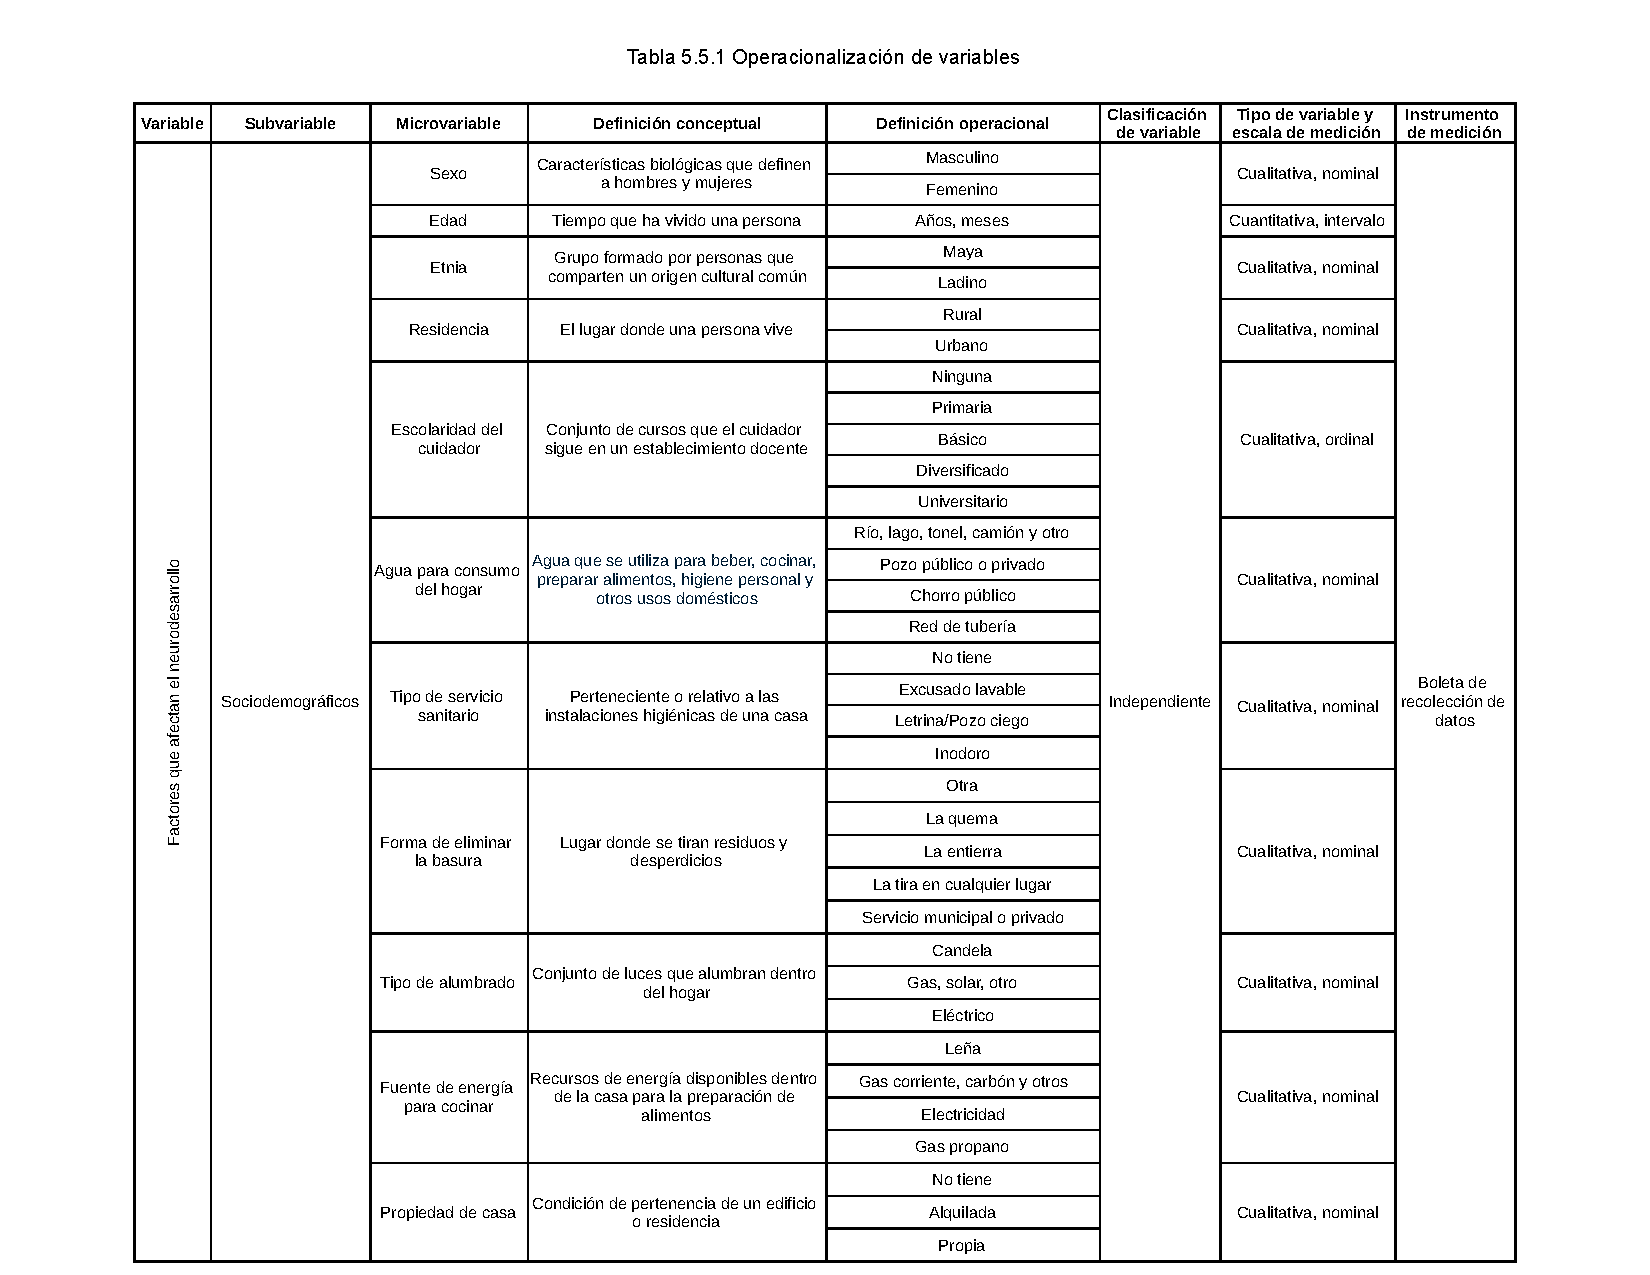
\includepdf[scale=0.93,landscape=true,pages=-,pagecommand={\thispagestyle{plain}}]{images/variables.pdf}

\section{Instrumentos utilizados en la recolección de la información}
Para este estudio se emplearon los siguientes instrumentos:
		\begin{itemize}
		\item \asq: Adaptado al idioma español y ajustado por edad.	
		\item Cuestionario de factores de riesgo.
		\end{itemize}

\section{Procedimientos para la recolección de información}
	\begin{enumerate}
		\item Fase preliminar (Febrero de 2025):
		Se obtuvieron los permisos correspondientes a las autoridades de salud
		del departamento de Quetzaltenango para acceder a los servicios de
		atención primaria seleccionados. Se determinaron estrategias para
		garantizar la uniformidad en la recolección de los datos entre los
		investigadores.
		\item Fase de recolección de datos:
		Se identificaron niños menores de 5 años que cumplieron con los
		criterios de inclusión en los servicios de atención primaria
		participantes. Tras obtener el consentimiento informado de los padres o
		tutores, se realizó:
			\begin{itemize}
			\item Evaluación del neurodesarrollo mediante la aplicación del
			\asq, seleccionando la versión específica según la edad del niño.
			\item Aplicación de un cuestionario estructurado para recolectar
			información sobre factores potencialmente asociados al
			neurodesarrollo.
			\end{itemize}
		\item Fase de clasificación y análisis:
		Los resultados de cada niño fueron evaluados conforme al puntaje
		obtenido en el \asq\ y clasificados en tres categorías:
			\begin{itemize}
			\item Desarrollo típico: puntaje en el área blanca, indicativo de
			un desarrollo acorde a su edad.
			\item Requiere monitoreo: puntaje en el área gris, señalando
			habilidades ligeramente por debajo del promedio.
			\item Retraso en el desarrollo: puntaje en el área negra,
			sugiriendo la necesidad de intervención especializada.
			\end{itemize}
		Se analizaron las asociaciones entre los factores de exposición
		identificados y los resultados de neurodesarrollo en la evaluación.
	\end{enumerate}

\section{Procedimientos de análisis de la información}
Los datos fueron recolectados utilizando la boleta de recolección de datos (ver
anexo D) la cual consiste en un formulario en línea.

Se realizó una limpieza inicial de datos para asegurar la consistencia de los
datos y evitar sesgo por entrada de datos.

Los puntajes obtenidos en cada área del desarrollo del \asq\ se convertieron a
puntajes Z de acuerdo a la ficha técnica de los cuestionarios. 
	
\subsection{Análisis descriptivo}
Se realizó un análisis descriptivo de la muestra, calculando frecuencias y
porcentajes para las variables categóricas, y medidas de tendencia central y
dispersión para las variables cuantitativas.

\subsection{Análisis inferencial}
Para evaluar la asociación entre los factores de riesgo (variables
independientes) y los resultados del \asq\ (variables dependientes), se
aplicaron las siguientes técnicas estadísticas:

\subsubsection{Prueba Chi-cuadrado de independencia}
Se utilizó esta prueba para analizar la asociación entre factores de riesgo
categóricos y los resultados del \asq\ dicotomizados (desarrollo adecuado/en
riesgo) y determinar la significancia estadística.

Para una población de \muestradeseada\ niños menores de 5 años, el
procedimiento para la prueba Chi-cuadrado fue el siguiente:

\begin{itemize}
    \item Se realizaron tablas de contingencia para cada par de variables
		categóricas (factor de riesgo y resultado del \asq).
    
    \item Se calculó el estadístico Chi-cuadrado mediante la fórmula:
    \[
    \chi^2 = \sum_{i=1}^r \sum_{j=1}^c \frac{(O_{ij} - E_{ij})^2}{E_{ij}}
    \]
    
    Donde \( O_{ij} \) son las frecuencias observadas y \( E_{ij} \) son las
	frecuencias esperadas bajo la hipótesis nula de independencia.
    
    \item Se estableció un nivel de significancia estadística de $\alpha = 0.05$
		para todas las pruebas, e intervalos de confianza de 95\% cálculados
		por el método del error estándar para describir el rango en el que se
		encuentra el valor real.
\end{itemize}

\subsection{Análisis de varianza (ANOVA)}
Para evaluar la relación entre factores de riesgo con múltiples categorías y
los resultados del neurodesarrollo cuantificados mediante puntajes Z del 
\asq, se utilizó el análisis de varianza (ANOVA) de una vía. Se utilizó esta
técnica estadística para determinar si existen diferencias significativas en las
medias de los puntajes Z entre tres o más grupos independientes, definidos por
las distintas categorías de los factores de riesgo.

El modelo matemático del ANOVA de un factor puede expresarse como:

\begin{equation}
Y_{ij} = \mu + \alpha_i + \varepsilon_{ij}
\end{equation}

Donde:
\begin{itemize}
    \item $Y_{ij}$ es la observación $j$-ésima en el $i$-ésimo grupo
    \item $\mu$ es la media general
    \item $\alpha_i$ es el efecto del factor de riesgo $i$
    \item $\varepsilon_{ij}$ es el error aleatorio que sigue una distribución $N(0, \sigma^2)$
\end{itemize}

El estadístico $F$ para el ANOVA se calcula como la razón entre la varianza
entre grupos y la varianza dentro de los grupos:

\begin{equation}
F = \frac{MS_{\text{entre}}}{MS_{\text{dentro}}} = \frac{\sum_{i=1}^{k} n_i(\bar{Y}_i - \bar{Y})^2/(k-1)}{\sum_{i=1}^{k}\sum_{j=1}^{n_i} (Y_{ij} - \bar{Y}_i)^2/(N-k)}
\end{equation}

Donde:
\begin{itemize}
    \item $MS_{\text{entre}}$ es la media cuadrática entre grupos
    \item $MS_{\text{dentro}}$ es la media cuadrática dentro de los grupos
    \item $k$ es el número de grupos
    \item $n_i$ es el tamaño de la muestra del grupo $i$
    \item $\bar{Y}_i$ es la media del grupo $i$
    \item $\bar{Y}$ es la media general
    \item $N$ es el tamaño total de la muestra
\end{itemize}

Dado que los tamaños muestrales no son homogéneos entre los diferentes grupos de
interés (debido a las características propias del muestreo en servicios de
atención primaria), se aplicó la prueba de Levene para evaluar si la
heterogenicidad de los resultados era significativa. 

\subsubsection{Prueba de Levene para homogeneidad de varianzas}
La prueba de Levene es una prueba estadística inferencial utilizada para
evaluar la igualdad de varianzas entre diferentes grupos. Esta prueba es menos
sensible a desviaciones de la normalidad que otras pruebas de igualdad de
varianzas, lo que la hace particularmente útil en el contexto de este estudio.

El procedimiento de la prueba de Levene implica:
\begin{itemize}
    \item Calcular la diferencia absoluta entre cada valor en un grupo y la
		media o mediana de ese grupo.
    \item Realizar un ANOVA de un factor sobre estos valores de diferencia
		absoluta.
    \item El estadístico resultante sigue una distribución F con k-1 y N-k
		grados de libertad, donde k es el número de grupos y N el tamaño total
		de la muestra.
\end{itemize}

Se interpretó el valor p de la prueba de Levene de la siguiente manera:
\begin{itemize}
    \item Si $p > 0.05$: No se rechaza la hipótesis nula de igualdad de
		varianzas, por lo que se procede con el ANOVA tradicional.
    \item Si $p \leq0.05$: Se rechaza la hipótesis nula, lo que indica que las
		varianzas no son iguales entre los grupos.
\end{itemize}

En caso de que no se cumpliera el supuesto de homogeneidad de varianzas, se
utilizó la prueba de Welch como alternativa al ANOVA tradicional. La prueba de
Welch realiza un ajuste de los grados de libertad para compensar la
heterogeneidad de varianzas, lo que la hace especialmente apropiada para
muestras con tamaños desiguales.

\subsubsection{Análisis post-hoc}
En los casos donde se encontraron diferencias significativas en el ANOVA
($p < 0.05$), se realizaron pruebas post-hoc Tukey HSD para identificar
específicamente entre qué grupos existen las diferencias.

\subsection{Análisis de asociación}
Se analizaron los resultados del \asq\ del grupo estudiado utilizando odds
ratio (OR): para comparar las probabilidades de que se presente riesgo en el
neurodesarrollo entre dos grupos diferentes. Por ejemplo para comparar si los
niños con padres que tienen un trabajo formal o informal tienen mayor
probabilidad o no, de presentar riesgo en el neurodesarrollo.

\subsection{Presentación de resultados}
Se elaboraron tablas y gráficos apropiados con intervalos utilizando
python y paquetes numpy, pandas, también se utilizó el software
Rstudio con paquetes de CRAN.

\section{Procedimientos para garantizar aspectos éticos de la investigación}
El presente estudio cumplió con los principios éticos fundamentales establecidos
para la investigación en seres humanos, se garantizó la protección de los
derechos, dignidad y bienestar de los participantes. A continuación, se
detallan los aspectos éticos considerados:

\subsection{Respeto por las personas}
Se aseguró el respeto a la autonomía de los cuidadores y los participantes al
obtener su consentimiento informado previo a la participación en el estudio.
En este documento se describieron claramente los objetivos, procedimientos,
beneficios y posibles riesgos del estudio.

\subsection{Confidencialidad y privacidad}
La privacidad de los participantes se respetó de forma estrica. Toda la
información recolectada fue tratada de manera confidencial y utilizada
únicamente con fines de investigación.

\subsection{Justicia}
Se garantizó que todos los niños elegibles tuviesen igualdad de oportunidades
para participar en el estudio, sin discriminación por razones de género, etnia,
nivel socioeconómico o creencias religiosas. Asimismo, los resultados del
estudio están orientados a beneficiar a la comunidad en general, fomentando
políticas y estrategias que mejoren el neurodesarrollo infantil.

\subsection{Beneficencia y no maleficencia}
Este estudio no implicó intervenciones invasivas ni riesgos significativos para
los participantes. Se emplearon técnicas observacionales y cuestionarios
validados que no afectan la salud o el bienestar de los niños ni de sus
cuidadores.

\subsection{Categoría de riesgo}
Categoría I: El diseño del estudio se basó en la aplicación del \asq\ el cual
es una herramienta validada y no invasiva para evaluar el neurodesarrollo
infantil. Este cuestionario se aplicó a los cuidadores (padres o tutores) de
los niños de forma observacional y no requirió intervención directa sobre los
participantes.

\subsection{Consentimiento informado}
Todos los cuidadores firmaron un consentimiento informado (ver anexo C) antes de
participar en el estudio.

\chapter{Resultados}

\begin{table}[htbp]
\centering
\caption{Distribución de Niños por Grupo de Edad y Sexo}
\label{tab:resultado1}
\begin{threeparttable}
\begin{tblr}{
  width = \linewidth,
  colspec = {X[2,c]X[1,c]X[1,c]X[1,c]X[1,c]X[1,c]X[1,c]},
  row{1} = {font=\bfseries, bg=gray!10},
  row{even} = {bg=gray!3},
  row{Z} = {font=\bfseries, bg=gray!15},
  cells = {valign=m, font=\footnotesize},
  hline{1,2,Z} = {1pt},
  hline{3-Y} = {0.5pt, gray},
}
\textbf{Grupo de Edad} & {\textbf{Femenino}\\n} & \textbf{Femenino (\%)} & {\textbf{Masculino}\\n} & \textbf{Masculino (\%)} & {\textbf{Total}\\n} & \textbf{Total (\%)} \\
0-2 meses & 43 & 2.49 & 39 & 2.26 & 82 & 4.75 \\
3-4 meses & 38 & 2.20 & 44 & 2.55 & 82 & 4.75 \\
5-6 meses & 53 & 3.07 & 46 & 2.67 & 99 & 5.74 \\
7-8 meses & 31 & 1.80 & 38 & 2.20 & 69 & 4.00 \\
9-10 meses & 67 & 3.88 & 59 & 3.42 & 126 & 7.30 \\
11-12 meses & 61 & 3.54 & 84 & 4.87 & 145 & 8.41 \\
13-16 meses & 63 & 3.65 & 73 & 4.23 & 136 & 7.88 \\
17-20 meses & 69 & 4.00 & 84 & 4.87 & 153 & 8.87 \\
21-24 meses & 79 & 4.58 & 93 & 5.39 & 172 & 9.97 \\
25-30 meses & 72 & 4.17 & 90 & 5.22 & 162 & 9.39 \\
31-36 meses & 75 & 4.35 & 108 & 6.26 & 183 & 10.61 \\
37-48 meses & 82 & 4.75 & 96 & 5.57 & 178 & 10.32 \\
49+ meses & 70 & 4.06 & 68 & 3.94 & 138 & 8.00 \\
\textbf{Total} & \textbf{803} & \textbf{46.55} & \textbf{922} & \textbf{53.45} & \textbf{1,725} & \textbf{100.0} \\
\end{tblr}
\begin{tablenotes}
\footnotesize
\item \textit{Fuente:} Boleta de recolección de datos.
\end{tablenotes}
\end{threeparttable}
\end{table}

\begin{table}[htbp]
\centering
\caption{Distribución de Niños de Acuerdo a Edad Gestacional}
\label{tab:eg}
\begin{threeparttable}
\begin{tblr}{
  width = 0.8\linewidth,
  colspec = {X[2,l]X[1,c]X[1,c]},
  row{1} = {font=\bfseries, bg=gray!10},
  row{even} = {bg=gray!3},
  cells = {valign=m, font=\footnotesize},
  hline{1,2,Z} = {1pt},
  hline{3-Y} = {0.5pt, gray},
}
\textbf{Categoría} & \textbf{Cantidad} & \textbf{Porcentaje (\%)} \\
A término & 1,545 & 89.5 \\
Pretérmino tardío & 114 & 6.6 \\
Pretérmino moderado & 57 & 3.3 \\
Muy pretérmino & 9 & 0.5 \\
\textbf{Total} & \textbf{1,725} & \textbf{100.0} \\
\end{tblr}
\begin{tablenotes}
\footnotesize
\item \textit{Criterios de clasificación:} A término (37-42 semanas), Pretérmino tardío (34-36 semanas), Pretérmino moderado (32-33 semanas), Muy pretérmino ($<$32 semanas).
\item \textit{Fuente:} Boleta de recolección de datos.
\end{tablenotes}
\end{threeparttable}
\end{table}

\begin{table}[htbp]
\centering
\caption{Distribución por Etnia y Área de Residencia}
\label{tab:etnia-residencia}
\begin{threeparttable}
\begin{tblr}{
  width = \linewidth,
  colspec = {X[2,l]X[1,c]X[1,c]X[1,c]X[1,c]},
  row{1} = {font=\bfseries, bg=gray!10},
  row{even} = {bg=gray!3},
  cells = {valign=m, font=\footnotesize},
  hline{1,2,Z} = {1pt},
  hline{3-Y} = {0.5pt, gray},
}
\textbf{Etnia} & {\textbf{Área Rural}\\n (\%)} & {\textbf{Área Urbana}\\n (\%)} & {\textbf{Total}\\n (\%)} \\
Indígena & 183 (71.2) & 558 (38.0) & 741 (42.96) \\
No indígena & 74 (28.8) & 910 (62.0) & 984 (57.04) \\
\textbf{Total} & \textbf{257 (14.90)} & \textbf{1,468 (85.10)} & \textbf{1,725 (100.0)} \\
\end{tblr}
\begin{tablenotes}
\footnotesize
\item \textit{Fuente:} Boleta de recolección de datos.
\end{tablenotes}
\end{threeparttable}
\end{table}

\begin{table}[htbp]
\centering
\caption{Distribución de Edad Materna y Paterna}
\label{tab:edad_padres}
\begin{threeparttable}
\begin{tblr}{
  width = 0.9\linewidth,
  colspec = {X[2,c]X[1,c]X[1,c]X[1,c]X[1,c]},
  row{1} = {font=\bfseries, bg=gray!10},
  row{even} = {bg=gray!3},
  cells = {valign=m, font=\footnotesize},
  hline{1,2,Z} = {1pt},
  hline{3-Y} = {0.5pt, gray},
}
{\textbf{Intervalo de}\\    \textbf{Edad (años)}} & {\textbf{Madres}\\n} & {\textbf{Madres}\\    \textbf{(\%)}} & {\textbf{Padres}\\n} & {\textbf{Padres}\\    \textbf{(\%)}} \\
14-19 & 104 & 6.1 & 40 & 2.4 \\
20-24 & 412 & 24.0 & 304 & 18.2 \\
25-29 & 548 & 32.0 & 457 & 27.3 \\
30-34 & 433 & 25.3 & 430 & 25.7 \\
35-39 & 180 & 10.5 & 292 & 17.4 \\
40-44 & 31 & 1.8 & 106 & 6.3 \\
45+ & 6 & 0.4 & 45 & 2.7 \\
\textbf{Total}\tnote{a} & \textbf{1,714} & \textbf{100.0} & \textbf{1,674} & \textbf{100.0} \\
\end{tblr}
\begin{tablenotes}
\footnotesize
\item[a] Datos disponibles para 1,714 madres y 1,674 padres de la muestra total de 1,725 niños.
\item \textit{Estadísticas descriptivas:} Edad materna promedio: 27.85 años (DE: 5.59); Edad paterna promedio: 30.42 años (DE: 6.64).
\item \textit{Fuente:} Boleta de recolección de datos.
\end{tablenotes}
\end{threeparttable}
\end{table}

\begin{table}[htbp]
\centering
\caption{Nivel Educativo Materno y Paterno}
\label{tab:escolaridad}
\begin{threeparttable}
\begin{tblr}{
  width = 0.9\linewidth,
  colspec = {X[2,l]X[1,c]X[1,c]X[1,c]X[1,c]},
  row{1} = {font=\bfseries, bg=gray!10},
  row{even} = {bg=gray!3},
  cells = {valign=m, font=\footnotesize},
  hline{1,2,Z} = {1pt},
  hline{3-Y} = {0.5pt, gray},
}
\textbf{Nivel Educativo} & {\textbf{Madre}\\n} & \textbf{Madre (\%)} & {\textbf{Padre}\\n} & \textbf{Padre (\%)} \\
Ninguna & 63 & 3.68 & 50 & 2.99 \\
Primaria & 315 & 18.38 & 259 & 15.49 \\
Básico & 507 & 29.58 & 380 & 22.73 \\
Diversificado & 701 & 40.90 & 811 & 48.50 \\
Universitario & 128 & 7.47 & 172 & 10.29 \\
\textbf{Total}\tnote{a} & \textbf{1,714} & \textbf{100.0} & \textbf{1,672} & \textbf{100.0} \\
\end{tblr}
\begin{tablenotes}
\footnotesize
\item[a] Datos disponibles para 1,714 madres y 1,672 padres de la muestra total.
\item \textit{Nota:} Los padres muestran mayor proporción de educación diversificada y universitaria comparado con las madres ($p < 0.05$).
\item \textit{Fuente:} Boleta de recolección de datos.
\end{tablenotes}
\end{threeparttable}
\end{table}

\begin{table}[htbp]
\centering
\caption{Condición Laboral Materna y Paterna}
\label{tab:empleo}
\begin{threeparttable}
\begin{tblr}{
  width = 0.9\linewidth,
  colspec = {X[2,l]X[1,c]X[1,c]X[1,c]X[1,c]},
  row{1} = {font=\bfseries, bg=gray!10},
  row{even} = {bg=gray!3},
  cells = {valign=m, font=\footnotesize},
  hline{1,2,Z} = {1pt},
  hline{3-Y} = {0.5pt, gray},
}
\textbf{Tipo de Empleo} & {\textbf{Madre}\\n} & \textbf{Madre (\%)} & {\textbf{Padre}\\n} & \textbf{Padre (\%)} \\
Trabajo formal & 504 & 29.65 & 1,056 & 63.01 \\
Trabajo informal & 346 & 20.35 & 464 & 27.68 \\
No trabaja & 850 & 50.00 & 156 & 9.31 \\
\textbf{Total}\tnote{a} & \textbf{1,700} & \textbf{100.0} & \textbf{1,676} & \textbf{100.0} \\
\end{tblr}
\begin{tablenotes}
\footnotesize
\item[a] Datos disponibles para 1,700 madres y 1,676 padres con información laboral completa.
\item \textit{Nota:} Diferencias significativas en patrones de empleo por género ($p < 0.001$, prueba de chi-cuadrado).
\item \textit{Fuente:} Boleta de recolección de datos.
\end{tablenotes}
\end{threeparttable}
\end{table}

\begin{table}[htbp]
\centering
\caption{Acceso a Servicios Básicos en el Hogar}
\label{tab:servicios_basicos}
\begin{threeparttable}
\begin{tblr}{
  width = \linewidth,
  colspec = {X[3,l]X[2,l]X[1,c]X[1,c]},
  row{1} = {font=\bfseries, bg=gray!10},
  row{even} = {bg=gray!3},
  cells = {valign=m, font=\footnotesize},
  hline{1,2,Z} = {1pt},
  hline{3-Y} = {0.5pt, gray},
}
\textbf{Variable} & \textbf{Categoría} & \textbf{Frecuencia} & \textbf{Porcentaje (\%)} \\
\textbf{Agua para consumo del hogar} & Red de tubería & 1,562 & 90.55 \\
& Chorro público & 142 & 8.23 \\
& Pozo público o privado & 18 & 1.04 \\
& Río, lago, tonel, camión y otro & 3 & 0.17 \\
\textbf{Tipo de servicio sanitario} & Inodoro & 1,615 & 93.62 \\
& Letrina/Pozo ciego & 109 & 6.32 \\
& Excusado lavable & 1 & 0.06 \\
\textbf{Eliminación de basura} & Servicio municipal o privado & 1,482 & 85.91 \\
& La quema & 223 & 12.93 \\
& La tira en cualquier lugar & 9 & 0.52 \\
& La entierra & 8 & 0.46 \\
& Otra & 3 & 0.17 \\
\textbf{Tipo de alumbrado} & Eléctrico & 1,725 & 100.0 \\
\textbf{Fuente de energía para cocinar} & Gas propano & 1,503 & 87.13 \\
& Leña & 216 & 12.52 \\
& Gas corriente, carbón y otros & 4 & 0.23 \\
& Electricidad & 2 & 0.12 \\
\end{tblr}
\begin{tablenotes}
\footnotesize
\item \textit{Fuente:} Boleta de recolección de datos.
\end{tablenotes}
\end{threeparttable}
\end{table}

\begin{table}[htbp]
\centering
\caption{Características de la Composición Familiar}
\label{tab:composicion_familiar}
\begin{threeparttable}
\begin{tblr}{
  width = \linewidth,
  colspec = {X[3,l]X[1,c]X[1,c]X[2,l]X[1,c]X[1,c]X[2,l]X[1,c]X[1,c]},
  row{1} = {font=\bfseries, bg=gray!10},
  row{even} = {bg=gray!3},
  cells = {valign=m, font=\scriptsize},
  hline{1,2,Z} = {1pt},
  hline{3-Y} = {0.5pt, gray},
}
{\textbf{Personas en}\\    \textbf{el hogar}} & \textbf{n} & \textbf{(\%)} & {\textbf{Número de}\\    \textbf{hermanos}} & \textbf{n} & \textbf{(\%)} & {\textbf{Posición}\\    \textbf{del niño}} & \textbf{n} & \textbf{(\%)} \\
1-2 & 1 & 0.06 & 0 & 540 & 31.3 & Primero & 694 & 40.23 \\
3-4 & 751 & 43.54 & 1 & 591 & 34.26 & Segundo & 616 & 35.71 \\
5-6 & 573 & 33.22 & 2 & 381 & 22.09 & Tercero & 372 & 21.57 \\
7-8 & 269 & 15.59 & 3 & 144 & 8.35 & Cuarto & 37 & 2.14 \\
9-10 & 68 & 3.94 & 4 & 47 & 2.72 & Quinto & 3 & 0.17 \\
11+ & 63 & 3.65 & 5 & 17 & 0.99 & Sexto & 2 & 0.12 \\
 & & & $\geq$6 & 5 & 0.29 & Séptimo+ & 1 & 0.06 \\
\textbf{Total} & \textbf{1,725} & \textbf{100.0} & \textbf{Total} & \textbf{1,725} & \textbf{100.0} & \textbf{Total} & \textbf{1,725} & \textbf{100.0} \\
\end{tblr}
\begin{tablenotes}
\footnotesize
\item \textit{Nota:} Promedio de personas por hogar: 5.32 (DE: 2.34); Promedio de hermanos: 1.21 (DE: 1.15).
\item \textit{Fuente:} Boleta de recolección de datos.
\end{tablenotes}
\end{threeparttable}
\end{table}

\begin{table}[htbp]
\centering
\caption{Acceso a Cuidados Prenatales}
\label{tab:cuidados_prenatales}
\begin{threeparttable}
\begin{tblr}{
  width = \linewidth,
  colspec = {X[2,l]X[1,c]X[1,c]X[3,l]X[1,c]X[1,c]},
  row{1} = {font=\bfseries, bg=gray!10},
  row{even} = {bg=gray!3},
  cells = {valign=m, font=\footnotesize},
  hline{1,2,Z} = {1pt},
  hline{3-Y} = {0.5pt, gray},
}
\textbf{Variable} & \textbf{Categoría} & \textbf{(\%)} & \textbf{Variable} & \textbf{Categoría} & \textbf{(\%)} \\
{\textbf{Controles}\\    \textbf{prenatales}} & 0 & 0.93 & {\textbf{Ultrasonido}\\    \textbf{obstétrico}} & No & 5.45 \\
& 1-2 & 4.46 & & Sí & 94.55 \\
& 3-4 & 22.49 & {\textbf{Vitaminas}\\    \textbf{(1er trimestre)}} & No & 11.83 \\
& 5-6 & 34.96 & & Sí & 88.17 \\
& 7-10 & 36.46 & {\textbf{Vitaminas}\\    \textbf{(resto embarazo)}} & No & 7.07 \\
& $\geq$11 & 0.70 & & Sí & 92.93 \\
\end{tblr}
\begin{tablenotes}
\footnotesize
\item \textit{Nota:} Promedio de controles prenatales: 6.70 (DE: 1.99).
\item \textit{Fuente:} Boleta de recolección de datos.
\end{tablenotes}
\end{threeparttable}
\end{table}

\begin{figure}[htbp]
    \centering
    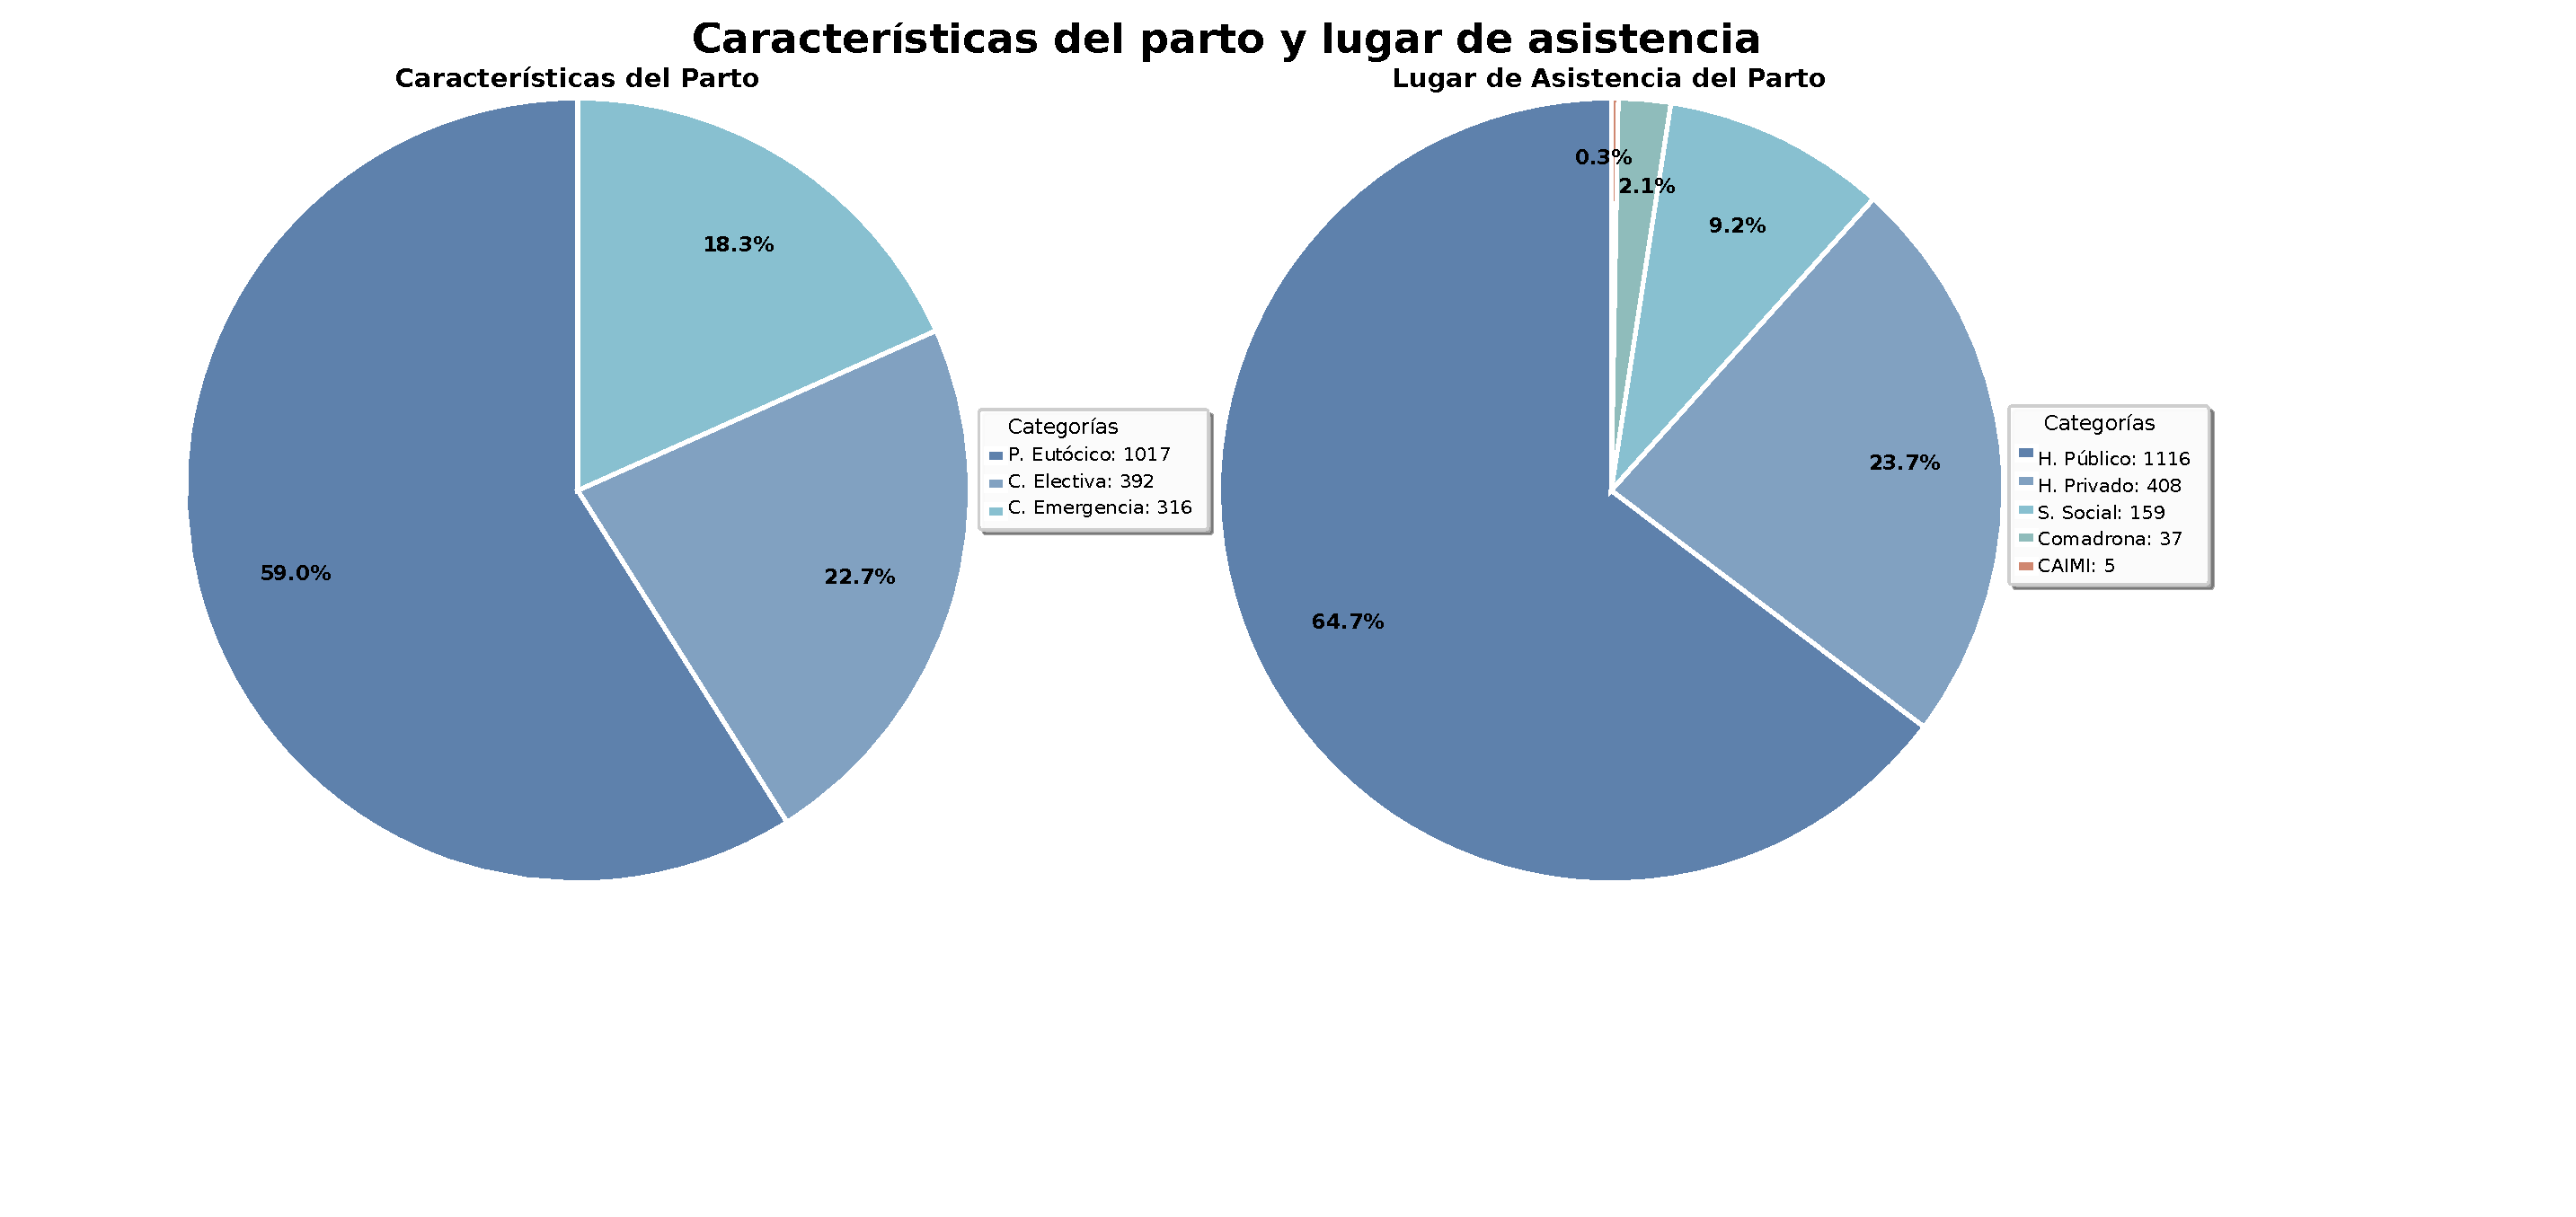
\includegraphics[width=1\textwidth]{grafica_asistencia_parto}
	\captionsetup{font=footnotesize}
    \caption{Distribución de lugar de asistencia y tipo de parto. Fuente: Boleta
	de recolección de datos.}
    \label{fig:parto}
\end{figure}

\begin{table}[htbp]
\centering
\caption{Causas de Césarea de Emergencia}
\label{tab:causas_cesarea}
\begin{threeparttable}
\begin{tblr}{
  width = \linewidth,
  colspec = {X[4,l]X[1,c]X[1,c]},
  row{1} = {font=\bfseries, bg=gray!10},
  row{even} = {bg=gray!3},
  cells = {valign=m, font=\footnotesize},
  hline{1,2,Z} = {1pt},
  hline{3-Y} = {0.5pt, gray},
}
\textbf{Categoría} & \textbf{Frecuencia} & \textbf{Porcentaje} \\
Complicaciones del líquido amniótico & 138 & 43.4\% \\
Sufrimiento fetal & 84 & 26.4\% \\
Preeclampsia & 36 & 11.3\% \\
Falta de progresión del trabajo de parto & 23 & 7.2\% \\
Presentación fetal anómala & 11 & 3.5\% \\
Ruptura pretérmino de membranas ovulares & 5 & 1.6\% \\
Problemas de placenta & 3 & 0.9\% \\
Embarazo múltiple & 2 & 0.6\% \\
Infección materna & 1 & 0.3\% \\
Otras causas & 14 & 4.4\% \\
\textbf{Total} & \textbf{317} & \textbf{100.0\%} \\
\end{tblr}
\begin{tablenotes}
\footnotesize
\item \textit{Nota:} Datos de acuerdo a 317 casos de césarea de emergencia de un total de 1,725 nacimientos.
\item \textit{Fuente:} Boleta de recolección de datos.
\end{tablenotes}
\end{threeparttable}
\end{table}

\begin{table}[htbp]
\centering
\caption{Patrones de Lactancia Durante los Primeros 24 Meses de Vida}
\label{tab:lactancia_periodos}
\begin{threeparttable}
\begin{tblr}{
  width = \linewidth,
  colspec = {X[3,l]X[1,c]X[1,c]X[1,c]},
  row{1} = {font=\bfseries, bg=gray!10},
  row{even} = {bg=gray!3},
  cells = {valign=m, font=\footnotesize},
  hline{1,2,Z} = {1pt},
  hline{3-Y} = {0.5pt, gray},
}
\textbf{Tipo de Lactancia} & {\textbf{0-6 meses}\\n (\%)} & {\textbf{6-12 meses}\\n (\%)} & {\textbf{12-24 meses}\\n (\%)} \\
Lactancia materna exclusiva & 1,254 (72.7) & 867 (55.6) & 609 (48.1) \\
Lactancia mixta & 336 (19.5) & 568 (36.4) & 547 (43.2) \\
Fórmula infantil & 135 (7.8) & 125 (8.0) & 101 (8.0) \\
Otro tipo de lactancia\tnote{a} & 0 (0.0) & 0 (0.0) & 8 (0.6) \\
\textbf{Total evaluado} & \textbf{1,725} & \textbf{1,560} & \textbf{1,265} \\
\end{tblr}
\begin{tablenotes}
\footnotesize
\item[a] Incluye leche de vaca, leche evaporada y otras alternativas.
\item \textit{Nota:} Las diferencias en el total se deben a la disponibilidad de datos según la edad del niño al momento de la evaluación.
\item \textit{Fuente:} Boleta de recolección de datos.
\end{tablenotes}
\end{threeparttable}
\end{table}

\begin{table}[htbp]
\centering
\caption{Cobertura de Suplementación con Vitamina A por Grupos de Edad}
\label{tab:vitamina_a}
\begin{threeparttable}
\begin{tblr}{
  width = 0.9\linewidth,
  colspec = {X[2,l]X[1,c]X[1,c]X[1,c]},
  row{1} = {font=\bfseries, bg=gray!10},
  row{even} = {bg=gray!3},
  cells = {valign=m, font=\footnotesize},
  hline{1,2,Z} = {1pt},
  hline{3-Y} = {0.5pt, gray},
}
\textbf{Estado de Suplementación} & {\textbf{6-12 meses}\\n (\%)} & {\textbf{12-18 meses}\\n (\%)} & {\textbf{18-24 meses}\\n (\%)} \\
Sí recibió & 1,088 (69.7) & 731 (57.7) & 554 (53.9) \\
No recibió & 473 (30.3) & 536 (42.3) & 474 (46.1) \\
\textbf{Total evaluado} & \textbf{1,561} & \textbf{1,267} & \textbf{1,028} \\
\end{tblr}
\begin{tablenotes}
\footnotesize
\item \textit{Fuente:} Boleta de recolección de datos.
\end{tablenotes}
\end{threeparttable}
\end{table}

\begin{table}[htbp]
\centering
\caption{Cobertura de Suplementación con Vitaminas y Minerales Espolvoreados}
\label{tab:vitaminas_minerales}
\begin{threeparttable}
\begin{tblr}{
  width = 0.9\linewidth,
  colspec = {X[2,l]X[1,c]X[1,c]X[1,c]},
  row{1} = {font=\bfseries, bg=gray!10},
  row{even} = {bg=gray!3},
  cells = {valign=m, font=\footnotesize},
  hline{1,2,Z} = {1pt},
  hline{3-Y} = {0.5pt, gray},
}
\textbf{Estado de Suplementación con Vitaminas y Minerales Espolvoreados} & {\textbf{6-12 meses}\\n (\%)} & {\textbf{12-18 meses}\\n (\%)} & {\textbf{18-24 meses}\\n (\%)} \\
Sí recibió & 1,078 (69.1) & 769 (60.7) & 553 (53.8) \\
No recibió o No los consumió & 483 (30.9) & 498 (39.3) & 474 (46.2) \\
\textbf{Total evaluado} & \textbf{1,561} & \textbf{1,267} & \textbf{1,027} \\
\end{tblr}
\begin{tablenotes}
\footnotesize
\item \textit{Fuente:} Boleta de recolección de datos.
\end{tablenotes}
\end{threeparttable}
\end{table}

\begin{table}[htbp]
\centering
\caption{Prevalencia de Antecedentes Nutricionales}
\label{tab:antecedentes_nutricionales}
\begin{threeparttable}
\begin{tblr}{
  width = 0.8\linewidth,
  colspec = {X[2,l]X[1,c]X[1,c]},
  row{1} = {font=\bfseries, bg=gray!10},
  row{even} = {bg=gray!3},
  cells = {valign=m, font=\footnotesize},
  hline{1,2,Z} = {1pt},
  hline{3-Y} = {0.5pt, gray},
}
\textbf{Antecedente Nutricional} & {\textbf{Retardo de}\\    \textbf{Crecimiento}\\n (\%)} & {\textbf{Desnutrición}\\    \textbf{Aguda}\\n (\%)} \\
Presente & 192 (11.1) & 102 (5.9) \\
Ausente & 1,533 (88.9) & 1,623 (94.1) \\
\textbf{Total} & \textbf{1,725 (100.0)} & \textbf{1,725 (100.0)} \\
\end{tblr}
\begin{tablenotes}
\footnotesize
\item \textit{Fuente:} Boleta de recolección de datos.
\end{tablenotes}
\end{threeparttable}
\end{table}

\begin{table}[htbp]
\centering
\caption{Prevalencia de Antecedentes de Hospitalización por Período}
\label{tab:hospitalizacion}
\begin{threeparttable}
\begin{tblr}{
  width = 0.9\linewidth,
  colspec = {X[2,l]X[1,c]X[1,c]},
  row{1} = {font=\bfseries, bg=gray!10},
  row{even} = {bg=gray!3},
  cells = {valign=m, font=\footnotesize},
  hline{1,2,Z} = {1pt},
  hline{3-Y} = {0.5pt, gray},
}
\textbf{Antecedente de Hospitalización} & {\textbf{Período Neonatal}\\    \textbf{(0-28 días)}\\n (\%)} & {\textbf{Infancia}\\    \textbf{($>$28 días)}\\n (\%)} \\
Sí presentó & 207 (12.0) & 237 (13.7) \\
No presentó & 1,518 (88.0) & 1,488 (86.3) \\
\textbf{Total} & \textbf{1,725 (100.0)} & \textbf{1,725 (100.0)} \\
\end{tblr}
\begin{tablenotes}
\footnotesize
\item \textit{Fuente:} Boleta de recolección de datos.
\end{tablenotes}
\end{threeparttable}
\end{table}

\begin{table}[htbp]
\centering
\caption{Principales Causas de Hospitalización por Período de Vida}
\label{tab:causas_hospitalizacion}
\begin{threeparttable}
\begin{tblr}{
  width = \linewidth,
  colspec = {X[1,l]X[1,l]},
  row{1} = {font=\bfseries, bg=gray!10},
  row{even} = {bg=gray!3},
  cells = {valign=t, font=\footnotesize},
  hline{1,2,Z} = {1pt},
  hline{3-Y} = {0.5pt, gray},
}
{\textbf{Período Neonatal}\\    \textbf{(n = 207)}} & {\textbf{Infancia}\\    \textbf{(n = 237)}} \\
\textbf{1.} Ictericia neonatal: 70 (33.8\%) & \textbf{1.} Neumonía: 119 (50.2\%) \\
\textbf{2.} Prematuridad: 61 (29.5\%) & \textbf{2.} Síndrome diarreico agudo: 53 (22.4\%) \\
\textbf{3.} Taquipnea transitoria: 50 (24.2\%) & \textbf{3.} Bronquiolitis: 48 (20.3\%) \\
\textbf{4.} Neumonía: 9 (4.3\%) & \textbf{4.} Fiebre de origen desconocido: 4 (1.7\%) \\
\textbf{5.} Síndrome de aspiración meconial: 5 (2.4\%) & \textbf{5.} Intolerancia a la lactosa: 2 (0.8\%) \\
\textbf{6.} Anomalías congénitas: 3 (1.4\%) & \textbf{6.} Hernioplastia: 2 (0.8\%) \\
\textbf{7.} Sepsis neonatal: 3 (1.4\%) & \textbf{7.} Sepsis: 2 (0.8\%) \\
\textbf{8.} Asfixia perinatal: 2 (1.0\%) & \textbf{8.} Apendicitis aguda: 2 (0.8\%) \\
{\textbf{Otros diagnósticos:} 4 (1.9\%)} & {\textbf{Otros diagnósticos:} 5 (2.1\%)} \\
\end{tblr}
\begin{tablenotes}
\footnotesize
\item \textit{Nota:} Las tres primeras causas representan el 87.5\% de hospitalizaciones neonatales y el 92.9\% de hospitalizaciones en la infancia.
\item \textit{Fuente:} Boleta de recolección de datos.
\end{tablenotes}
\end{threeparttable}
\end{table}

\begin{table}[htbp]
\centering
\caption{Estado de Vacunación}
\label{tab:vacunacion}
\begin{threeparttable}
\begin{tblr}{
  width = 0.7\linewidth,
  colspec = {X[2,l]X[1,c]},
  row{1} = {font=\bfseries, bg=gray!10},
  row{even} = {bg=gray!3},
  cells = {valign=m, font=\footnotesize},
  hline{1,2,Z} = {1pt},
  hline{3-Y} = {0.5pt, gray},
}
\textbf{Estado de Vacunación} & \textbf{Casos n (\%)} \\
Esquema completo para la edad & 1,637 (94.9) \\
Esquema incompleto & 88 (5.1) \\
\textbf{Total} & \textbf{1,725 (100.0)} \\
\end{tblr}
\begin{tablenotes}
\footnotesize
\item \textit{Nota:} Evaluación de acuerdo al esquema nacional de vacunación vigente según la edad del niño al momento del estudio.
\item \textit{Fuente:} Boleta de recolección de datos.
\end{tablenotes}
\end{threeparttable}
\end{table}

\begin{table}[htbp]
\centering
\caption{Estadísticas Descriptivas de Exposición a Pantallas y Tiempo de Juego con el Cuidador}
\label{tab:tiempo_pantallas_juego}
\begin{threeparttable}
\begin{tblr}{
  width = \linewidth,
  colspec = {X[2,l]X[1,c]X[1,c]},
  row{1} = {font=\bfseries, bg=gray!10},
  row{even} = {bg=gray!3},
  cells = {valign=m, font=\footnotesize},
  hline{1,2,Z} = {1pt},
  hline{3-Y} = {0.5pt, gray},
}
\textbf{Estadística} & {\textbf{Exposición a Pantallas}\\    \textbf{Electrónicas (horas)}} & {\textbf{Tiempo de Juego con}\\    \textbf{el Cuidador (horas)}} \\
n (muestra) & 1,725 & 1,725 \\
Media & 1.09 & 2.61 \\
Desviación estándar & 1.29 & 1.32 \\
Mínimo & 0.0 & 0.0 \\
Percentil 25 & 0.0 & 2.0 \\
Mediana (P50) & 1.0 & 3.0 \\
Percentil 75 & 2.0 & 3.0 \\
Máximo & 12.0 & 10.0 \\
Rango intercuartílico & 2.0 & 1.0 \\
\end{tblr}
\begin{tablenotes}
\footnotesize
\item \textit{Fuente:} Boleta de recolección de datos.
\end{tablenotes}
\end{threeparttable}
\end{table}

\begin{table}[htbp]
\centering
\caption{Evaluación del Desarrollo Infantil por Dominios Específicos}
\label{tab:desarrollo_dominios}
\begin{threeparttable}
\begin{tblr}{
  width = \linewidth,
  colspec = {X[2,l]X[1,c]X[1,c]X[1,c]},
  row{1} = {font=\bfseries, bg=gray!10},
  row{even} = {bg=gray!3},
  cells = {valign=m, font=\footnotesize},
  hline{1,2,Z} = {1pt},
  hline{3-Y} = {0.5pt, gray},
}
\textbf{Dominio del Desarrollo} & {\textbf{Desarrollo}\\    \textbf{Adecuado}\\n (\%)} & {\textbf{Desarrollo}\\    \textbf{en Riesgo}\\n (\%)} & {\textbf{Desarrollo en}\\    \textbf{Alto Riesgo}\\n (\%)} \\
Comunicación & 1,628 (94.4) & 83 (4.8) & 14 (0.8) \\
Resolución de problemas & 1,597 (92.6) & 116 (6.7) & 12 (0.7) \\
Desarrollo socio-individual & 1,600 (92.8) & 108 (6.3) & 17 (1.0) \\
Motricidad fina & 1,577 (91.4) & 124 (7.2) & 24 (1.4) \\
Motricidad gruesa & 1,437 (83.3) & 234 (13.6) & 54 (3.1) \\
\end{tblr}
\begin{tablenotes}
\footnotesize
\item \textit{Criterios de clasificación:} Desarrollo adecuado ($Z > -1$), Desarrollo en riesgo ($-2 < Z \leq -1$), Desarrollo en alto riesgo ($Z \leq -2$)..
\item \textit{Fuente:} Boleta de recolección de datos y Cuestionario Edades y Etapas 3.
\end{tablenotes}
\end{threeparttable}
\end{table}

\begin{table}[htbp]
\centering
\caption{Clasificación Global del Desarrollo Infantil}
\label{tab:desarrollo_global}
\begin{threeparttable}
\begin{tblr}{
  width = 0.8\linewidth,
  colspec = {X[2,l]X[1,c]X[1,c]},
  row{1} = {font=\bfseries, bg=gray!10},
  row{even} = {bg=gray!3},
  cells = {valign=m, font=\footnotesize},
  hline{1,2,Z} = {1pt},
  hline{3-Y} = {0.5pt, gray},
}
\textbf{Clasificación Global} & \textbf{Frecuencia} & \textbf{Porcentaje} \\
Desarrollo adecuado global\tnote{a} & 1,155 & 66.96 \\
Riesgo en cualquier dominio\tnote{b} & 570 & 33.04 \\
Alto riesgo en cualquier dominio\tnote{c} & 90 & 5.22 \\
\textbf{Total} & \textbf{1,725} & \textbf{100.00} \\
\end{tblr}
\begin{tablenotes}
\footnotesize
\item[a] Todos los dominios con $Z > -1$
\item[b] Al menos un dominio con $Z \leq -1$
\item[c] Al menos un dominio con $Z \leq -2$
\item \textit{Nota:} Los casos de alto riesgo están incluidos en la categoría de riesgo general.
\item \textit{Fuente:} Resultados del Cuestionario edades y etapas 3.
\end{tablenotes}
\end{threeparttable}
\end{table}

\begin{table}[htbp]
\centering
\caption{Estadísticas Descriptivas de los Puntajes Z por Dominios del Desarrollo}
\label{tab:estadisticas_z_scores}
\begin{threeparttable}
\begin{tblr}{
  width = \linewidth,
  colspec = {X[2,l]X[1,c]X[1,c]X[1,c]X[1,c]X[1,c]},
  row{1} = {font=\bfseries, bg=gray!10},
  row{even} = {bg=gray!3},
  cells = {valign=m, font=\footnotesize},
  hline{1,2,Z} = {1pt},
  hline{3-Y} = {0.5pt, gray},
}
\textbf{Estadística} & {\textbf{Comunicación}\\Z-score} & {\textbf{Motricidad}\\    \textbf{Gruesa}\\Z-score} & {\textbf{Motricidad}\\    \textbf{Fina}\\Z-score} & {\textbf{Resolución de}\\    \textbf{Problemas}\\Z-score} & {\textbf{Desarrollo}\\    \textbf{Socio-Individual}\\Z-score} \\
n (muestra) & 1,725 & 1,725 & 1,725 & 1,725 & 1,725 \\
Media & 0.111 & $-0.269$ & $-0.077$ & $-0.068$ & 0.034 \\
Desviación estándar & 0.691 & 0.832 & 0.729 & 0.682 & 0.719 \\
Mínimo & $-4.357$ & $-6.724$ & $-4.684$ & $-4.540$ & $-4.813$ \\
Percentil 25 & $-0.263$ & $-0.698$ & $-0.489$ & $-0.449$ & $-0.383$ \\
Mediana (P50) & 0.135 & $-0.208$ & $-0.024$ & $-0.036$ & $-0.029$ \\
Percentil 75 & 0.631 & 0.373 & 0.495 & 0.396 & 0.639 \\
Máximo & 1.745 & 1.228 & 1.284 & 1.383 & 1.488 \\
Rango intercuartílico & 0.894 & 1.071 & 0.984 & 0.845 & 1.022 \\
\end{tblr}
\begin{tablenotes}
\footnotesize
\item \textit{Interpretación clínica:} Los puntajes Z representan desviaciones estándar respecto a la media poblacional normalizada. Valores negativos indican rendimiento por debajo del promedio esperado.
\item \textit{Criterios de riesgo:} $Z \leq -1$ (riesgo), $Z \leq -2$ (alto riesgo). Motricidad gruesa presenta la media más baja ($-0.269$), indicando mayor vulnerabilidad en este dominio.
\item \textit{Normalidad:} Todas las distribuciones en los diferentes dominios pasan la prueba de Kolmogorov-Smirnov ($p > 0.05$), confirmando distribución aproximadamente normal.
\item \textit{Fuente:} Análisis estadístico de resultados de los Cuestionarios Edades y Etapas 3.
\end{tablenotes}
\end{threeparttable}
\end{table}

\begin{figure}[htbp]
    \centering
    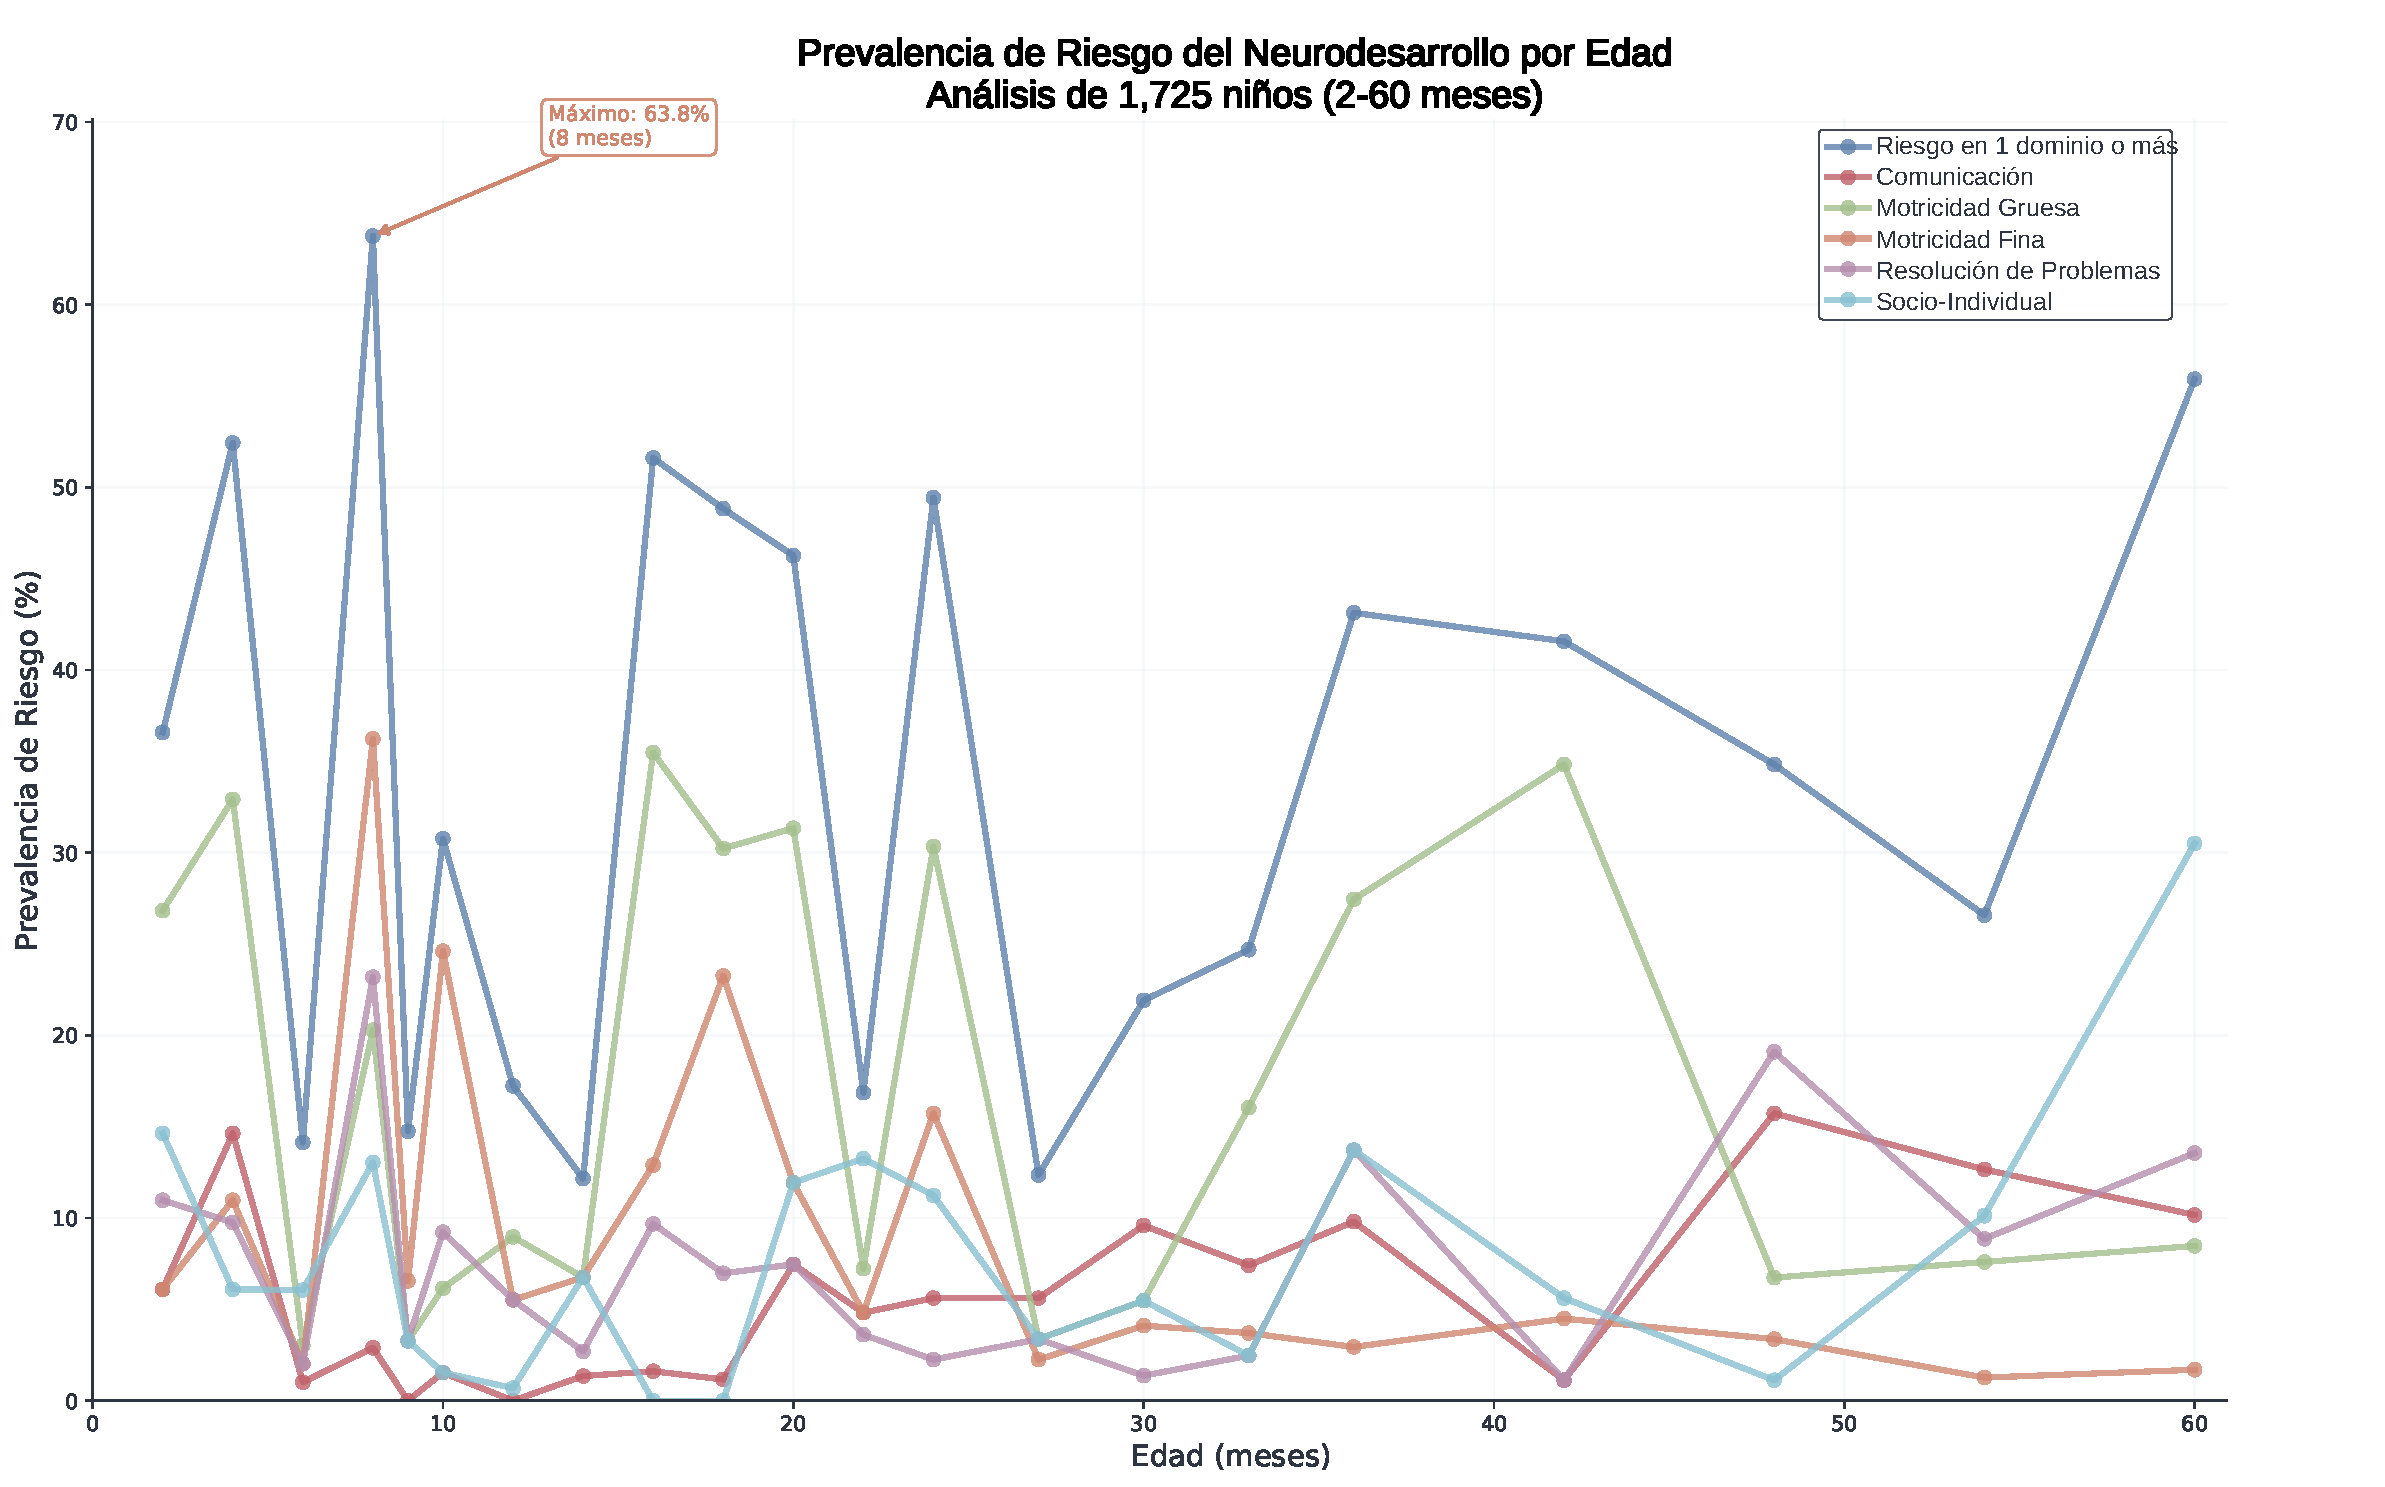
\includegraphics[width=1\textwidth]{prevalencia_edad_nord}
	\captionsetup{font=footnotesize}
	\caption{Prevalencia de riesgo en el desarrollo de acuerdo a rangos de edad
	del ASQ-3.}
    \label{fig:prevalencia_riesgo_asq3}
\end{figure}

\begin{figure}[htbp]
    \centering
    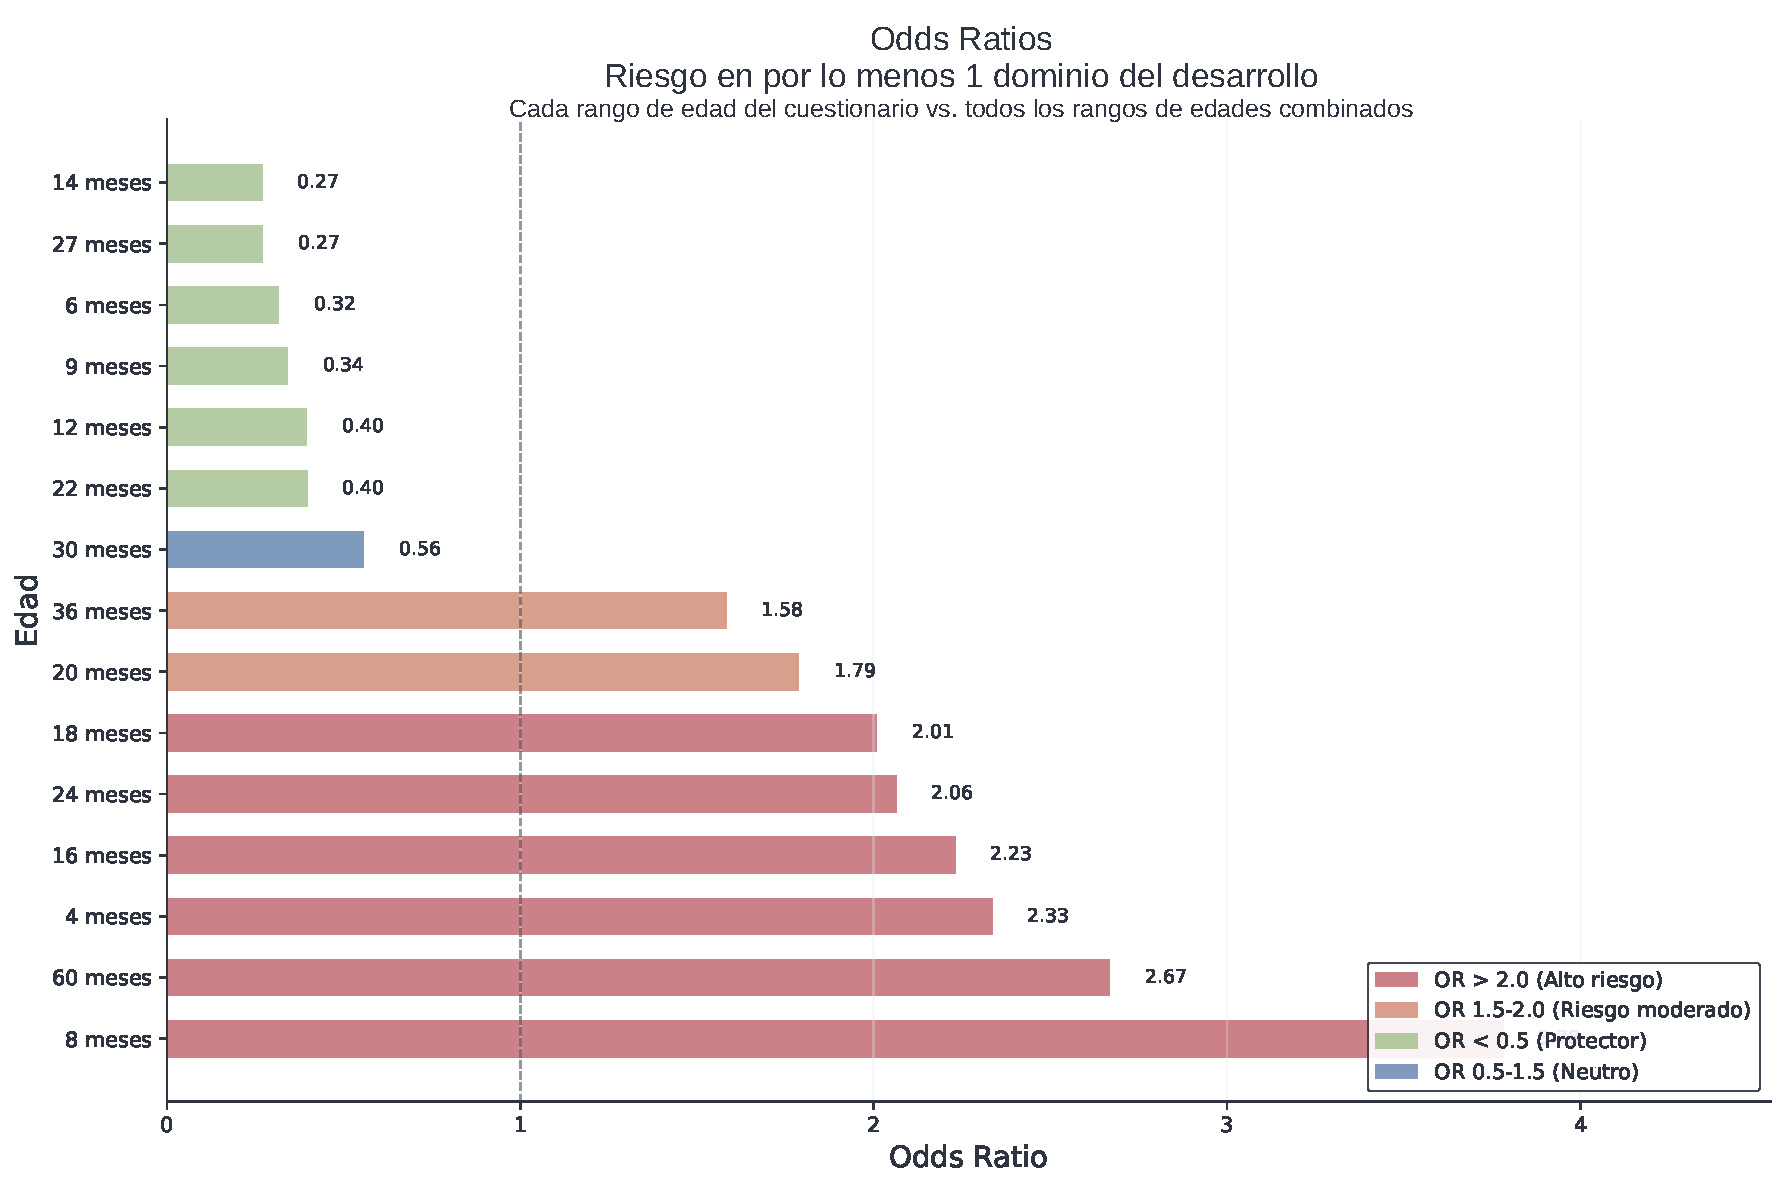
\includegraphics[width=1\textwidth]{odds_ratios_nord}
	\captionsetup{font=footnotesize}
	\caption{Odds ratio de presentar al menos 1 dominio en riesgo de acuerdo a
	los rangos de edades evaluados por los cuestionarios ASQ-3.}
    \label{fig:odds_ratio_asq3}
\end{figure}

\begin{table}[htbp]
\centering
\caption{Distribución y Asociación de la Variable \textit{Sexo del Niño} con los Dominios del Desarrollo}
\label{tab:sexo_nino_desarrollo_chi2}
\begin{threeparttable}
\begin{tblr}{
  width = \linewidth,
  colspec = {X[2,l]X[1,c]X[1,c]X[1,c]X[1,c]X[1,c]X[1,c]X[1,c]},
  row{1} = {font=\bfseries, bg=gray!10},
  row{even} = {bg=gray!3},
  cells = {valign=m, font=\footnotesize},
  hline{1,2,Z} = {1pt},
  hline{3-Y} = {0.5pt, gray},
}
\textbf{Dominio} & \textbf{Sexo} & \textbf{Desarrollo Adecuado} & \textbf{En Riesgo} & \textbf{Alto Riesgo} & \textbf{Total} & $\chi^2$ & \textit{p}-valor \\
Comunicación          & Femenino    & 765 & 34  & 4  & 803 & 2.986 & 0.225 \\
                      & Masculino   & 863 & 49  & 10 & 922 &       &       \\
                      & \textbf{Total}      & \textbf{1628} & \textbf{83}  & \textbf{14} & \textbf{1725} &       &       \\
Motricidad Gruesa     & Femenino    & 669 & 105 & 29 & 803 & 1.376 & 0.503 \\
                      & Masculino   & 768 & 129 & 25 & 922 &       &       \\
                      & \textbf{Total}      & \textbf{1437} & \textbf{234} & \textbf{54} & \textbf{1725} &       &       \\
Motricidad Fina       & Femenino    & 741 & 51  & 11 & 803 & 1.591 & 0.451 \\
                      & Masculino   & 836 & 73  & 13 & 922 &       &       \\
                      & \textbf{Total}      & \textbf{1577} & \textbf{124} & \textbf{24} & \textbf{1725} &       &       \\
Resolución de Problemas & Femenino  & 751 & 47  & 5  & 803 & 1.957 & 0.376 \\
                      & Masculino   & 846 & 69  & 7  & 922 &       &       \\
                      & \textbf{Total}      & \textbf{1597} & \textbf{116} & \textbf{12} & \textbf{1725} &       &       \\
Socio-Individual      & Femenino    & 745 & 49  & 9  & 803 & 0.340 & 0.844 \\
                      & Masculino   & 855 & 59  & 8  & 922 &       &       \\
                      & \textbf{Total}      & \textbf{1600} & \textbf{108} & \textbf{17} & \textbf{1725} &       &       \\
\end{tblr}
\begin{tablenotes}
\footnotesize
\item \textbf{Método:} Prueba Chi-cuadrado.
\item \textbf{Nota:} Todas las asociaciones entre sexo y dominio de desarrollo NO fueron estadísticamente significativas (\textit{p} $>$ 0.05).
\end{tablenotes}
\end{threeparttable}
\end{table}

\begin{table}[htbp]
\centering
\caption{Asociación entre grupo étnico y riesgo en dominios del desarrollo}
\label{tab:grupo_etnico_desarrollo_chi2_compacta}
\begin{threeparttable}
\begin{tblr}{
  width = 0.75\linewidth,
  colspec = {X[1.5,l]X[1.0,c]X[1.1,c]X[1.0,c]X[1.3,c]X[1.1,c]},
  row{1} = {font=\bfseries, bg=gray!10},
  row{even} = {bg=gray!3},
  cells = {valign=m, font=\footnotesize},
  hline{1,2,Z} = {1pt},
  hline{3-Y} = {0.5pt, gray},
}
\textbf{Dominio} & \textbf{$\chi^2$} & \textbf{\textit{p}-valor} & \textbf{OR} & \textbf{IC 95\%} & \textbf{Significativo} \\
Comunicación          & 2.73   & 0.098     & --    & --            & No \\
Motricidad gruesa     & 0.39   & 0.533     & --    & --            & No \\
Motricidad fina       & 1.89   & 0.169     & --    & --            & No \\
Resolución de problemas & 4.57   & 0.033     & 1.50  & 1.05--2.16    & Sí \\
Socio-individual      & 4.90   & 0.027     & 1.53  & 1.06--2.21    & Sí \\
\end{tblr}
\begin{tablenotes}
\footnotesize
\item \textbf{Método:} Prueba Chi-cuadrado.
\item \textbf{Interpretación:}
No se encontró asociación significativa en Comunicación (OR no aplicable, $\chi^2$ = 2.73, \textit{p} = 0.098), Motricidad gruesa (OR no aplicable, $\chi^2$ = 0.39, \textit{p} = 0.533) ni Motricidad fina (OR no aplicable, $\chi^2$ = 1.89, \textit{p} = 0.169).
En Resolución de problemas, el riesgo fue 1.50 veces mayor en el grupo indígena (OR = 1.50, IC 95\%: 1.05--2.16). En Socio-individual, el riesgo fue 1.53 veces mayor en el grupo indígena (OR = 1.53, IC 95\%: 1.06--2.21).
\end{tablenotes}
\end{threeparttable}
\end{table}

\begin{table}[htbp]
\centering
\caption{Asociación entre área de residencia y riesgo en dominios del desarrollo}
\label{tab:area_residencia_desarrollo_chi2_compacta}
\begin{threeparttable}
\begin{tblr}{
  width = 0.75\linewidth,
  colspec = {X[1.5,l]X[1.0,c]X[1.1,c]X[1.0,c]X[1.3,c]X[1.1,c]},
  row{1} = {font=\bfseries, bg=gray!10},
  row{even} = {bg=gray!3},
  cells = {valign=m, font=\footnotesize},
  hline{1,2,Z} = {1pt},
  hline{3-Y} = {0.5pt, gray},
}
\textbf{Dominio} & \textbf{$\chi^2$} & \textbf{\textit{p}-valor} & \textbf{OR} & \textbf{IC 95\%} & \textbf{Significativo} \\
Comunicación          & 8.70   & 0.003     & 2.09  & 1.30--3.36    & Sí \\
Motricidad gruesa     & 12.62  & $<$0.001  & 1.79  & 1.31--2.46    & Sí \\
Motricidad fina       & 1.73   & 0.188     & --    & --            & No \\
Resolución de problemas & 25.13  & $<$0.001  & 2.77  & 1.85--4.15    & Sí \\
Socio-individual      & 15.06  & $<$0.001  & 2.31  & 1.52--3.51    & Sí \\
\end{tblr}
\begin{tablenotes}
\footnotesize
\item \textbf{Método:} Prueba Chi-cuadrado.
\item \textbf{Nota:}
Se observó asociación significativa entre área de residencia y riesgo en Comunicación (OR = 2.09, IC 95\%: 1.30--3.36), Motricidad gruesa (OR = 1.79, IC 95\%: 1.31--2.46), Resolución de problemas (OR = 2.77, IC 95\%: 1.85--4.15) y Socio-individual (OR = 2.31, IC 95\%: 1.52--3.51) (\textit{p} $<$ 0.01). El riesgo de retraso fue mayor en el área rural.
En Motricidad fina, no se encontró asociación significativa (OR no significativo, $\chi^2$ = 1.73, \textit{p} = 0.188).
\end{tablenotes}
\end{threeparttable}
\end{table}

\begin{table}[htbp]
\centering
\caption{Asociación entre estado civil del cuidador y riesgo en dominios del desarrollo}
\label{tab:estado_civil_cuidador_desarrollo}
\begin{threeparttable}
\begin{tblr}{
  width = 0.95\linewidth,
  colspec = {X[1.4,l]X[0.8,c]X[1.0,c]X[1.0,c]X[1.0,c]X[0.7,c]},
  row{1} = {font=\bfseries, bg=gray!10},
  row{even} = {bg=gray!3},
  cells = {valign=m, font=\footnotesize},
  hline{1,2,Z} = {1pt},
  hline{3-Y} = {0.5pt, gray},
}
\textbf{Dominio} & \textbf{F/W} & \textbf{\textit{p}-valor} & \textbf{Significativo} & \textbf{Método} & \textbf{N} \\
Comunicación          & 10.18   & $<$0.001  & Sí  & Welch's ANOVA & 1725 \\
Motricidad gruesa     & 5.03    & 0.007     & Sí  & ANOVA         & 1725 \\
Motricidad fina       & 1.60    & 0.202     & No  & ANOVA         & 1725 \\
Resolución de problemas & 6.12  & 0.002     & Sí  & Welch's ANOVA & 1725 \\
Socio-individual      & 3.88    & 0.021     & Sí  & ANOVA         & 1725 \\
\end{tblr}
\begin{tablenotes}
\footnotesize
\item \textbf{Nota}: Se observó asociación significativa en los dominios de
comunicación, motor gruesa, resolución de problemas y socio-individual. Los
niños de cuidadores solteros presentaron menores medias de puntajes Z en
dominios de comunicación, resolución de problemas y socio-individual;
cuidadores casados presentaron menores puntajes Z en motricidad gruesa.
El grupo de niños de cuidadores unidos presentaron mayores medias Z y menor
proporción de riesgo en comunicación, resolución de problemas y
socio-individual.
\end{tablenotes}
\end{threeparttable}
\end{table}

\begin{figure}[htbp]
    \centering
    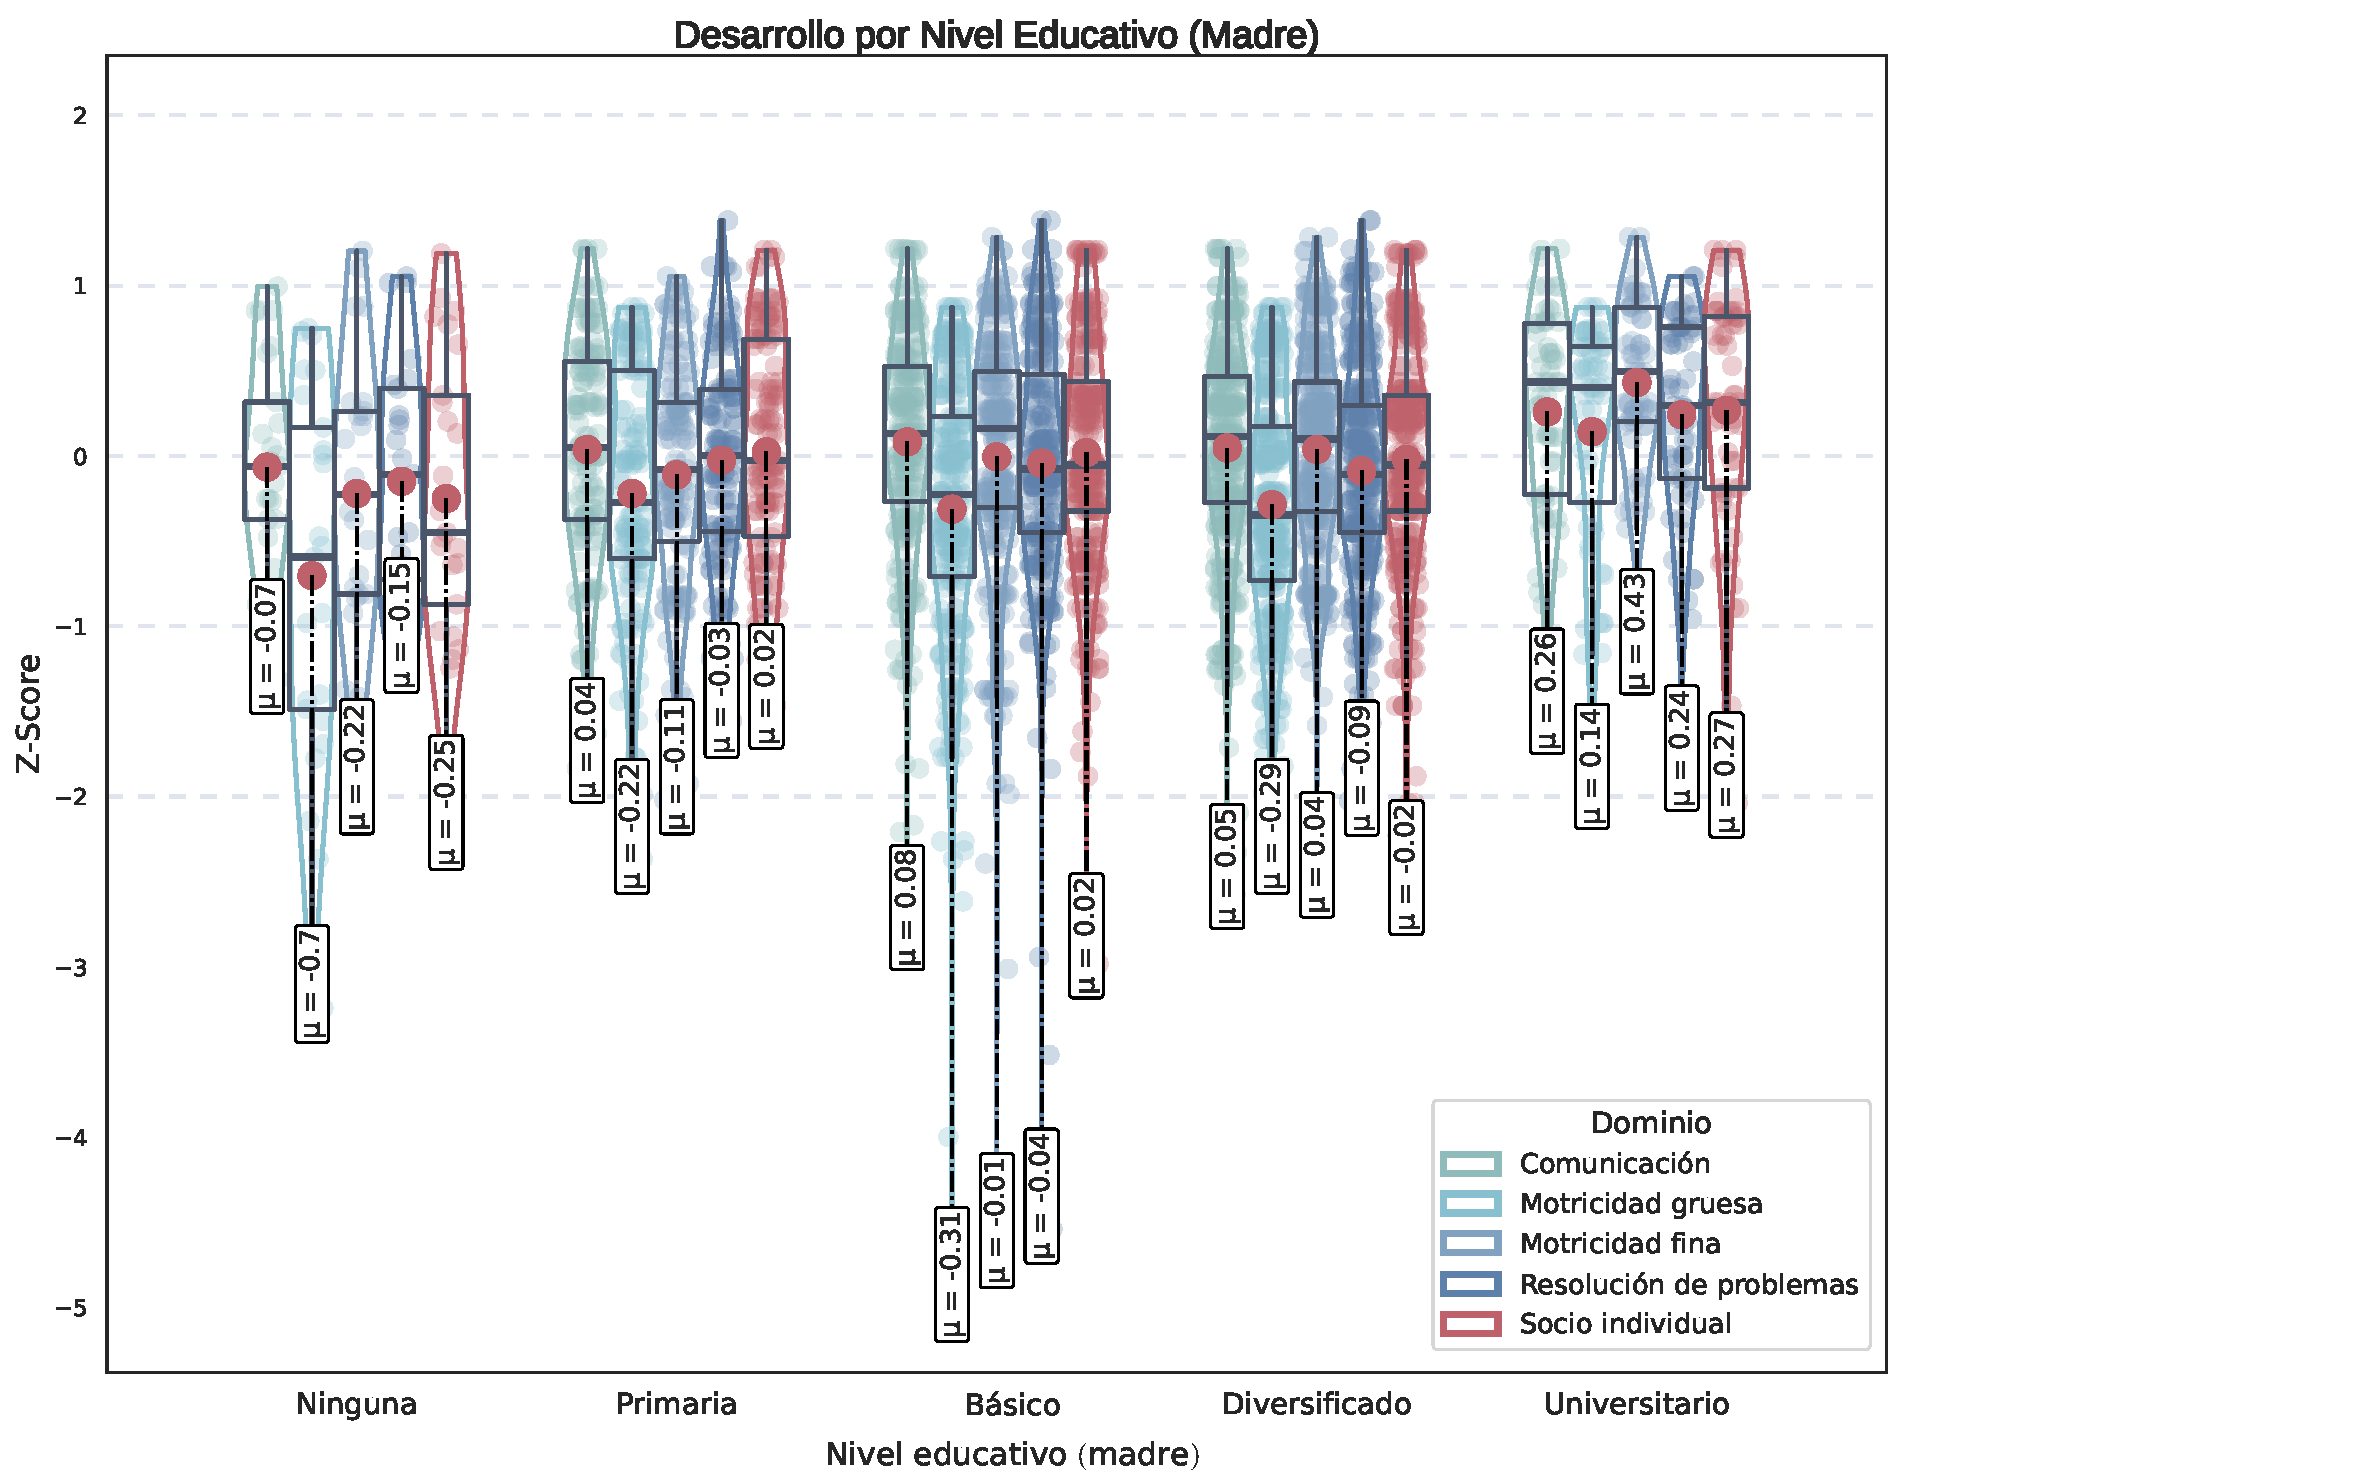
\includegraphics[width=1\textwidth]{violinplot_nivel_educativo_madre}
	\captionsetup{font=footnotesize}
	\caption{Desarrollo por nivel educativo (madre). Fuente: Cuadro \ref{tab:nivel_educativo_madre_desarrollo_anova}}
    \label{fig:nivel_educativo_anova_madre}
\end{figure}

\begin{figure}[htbp]
    \centering
    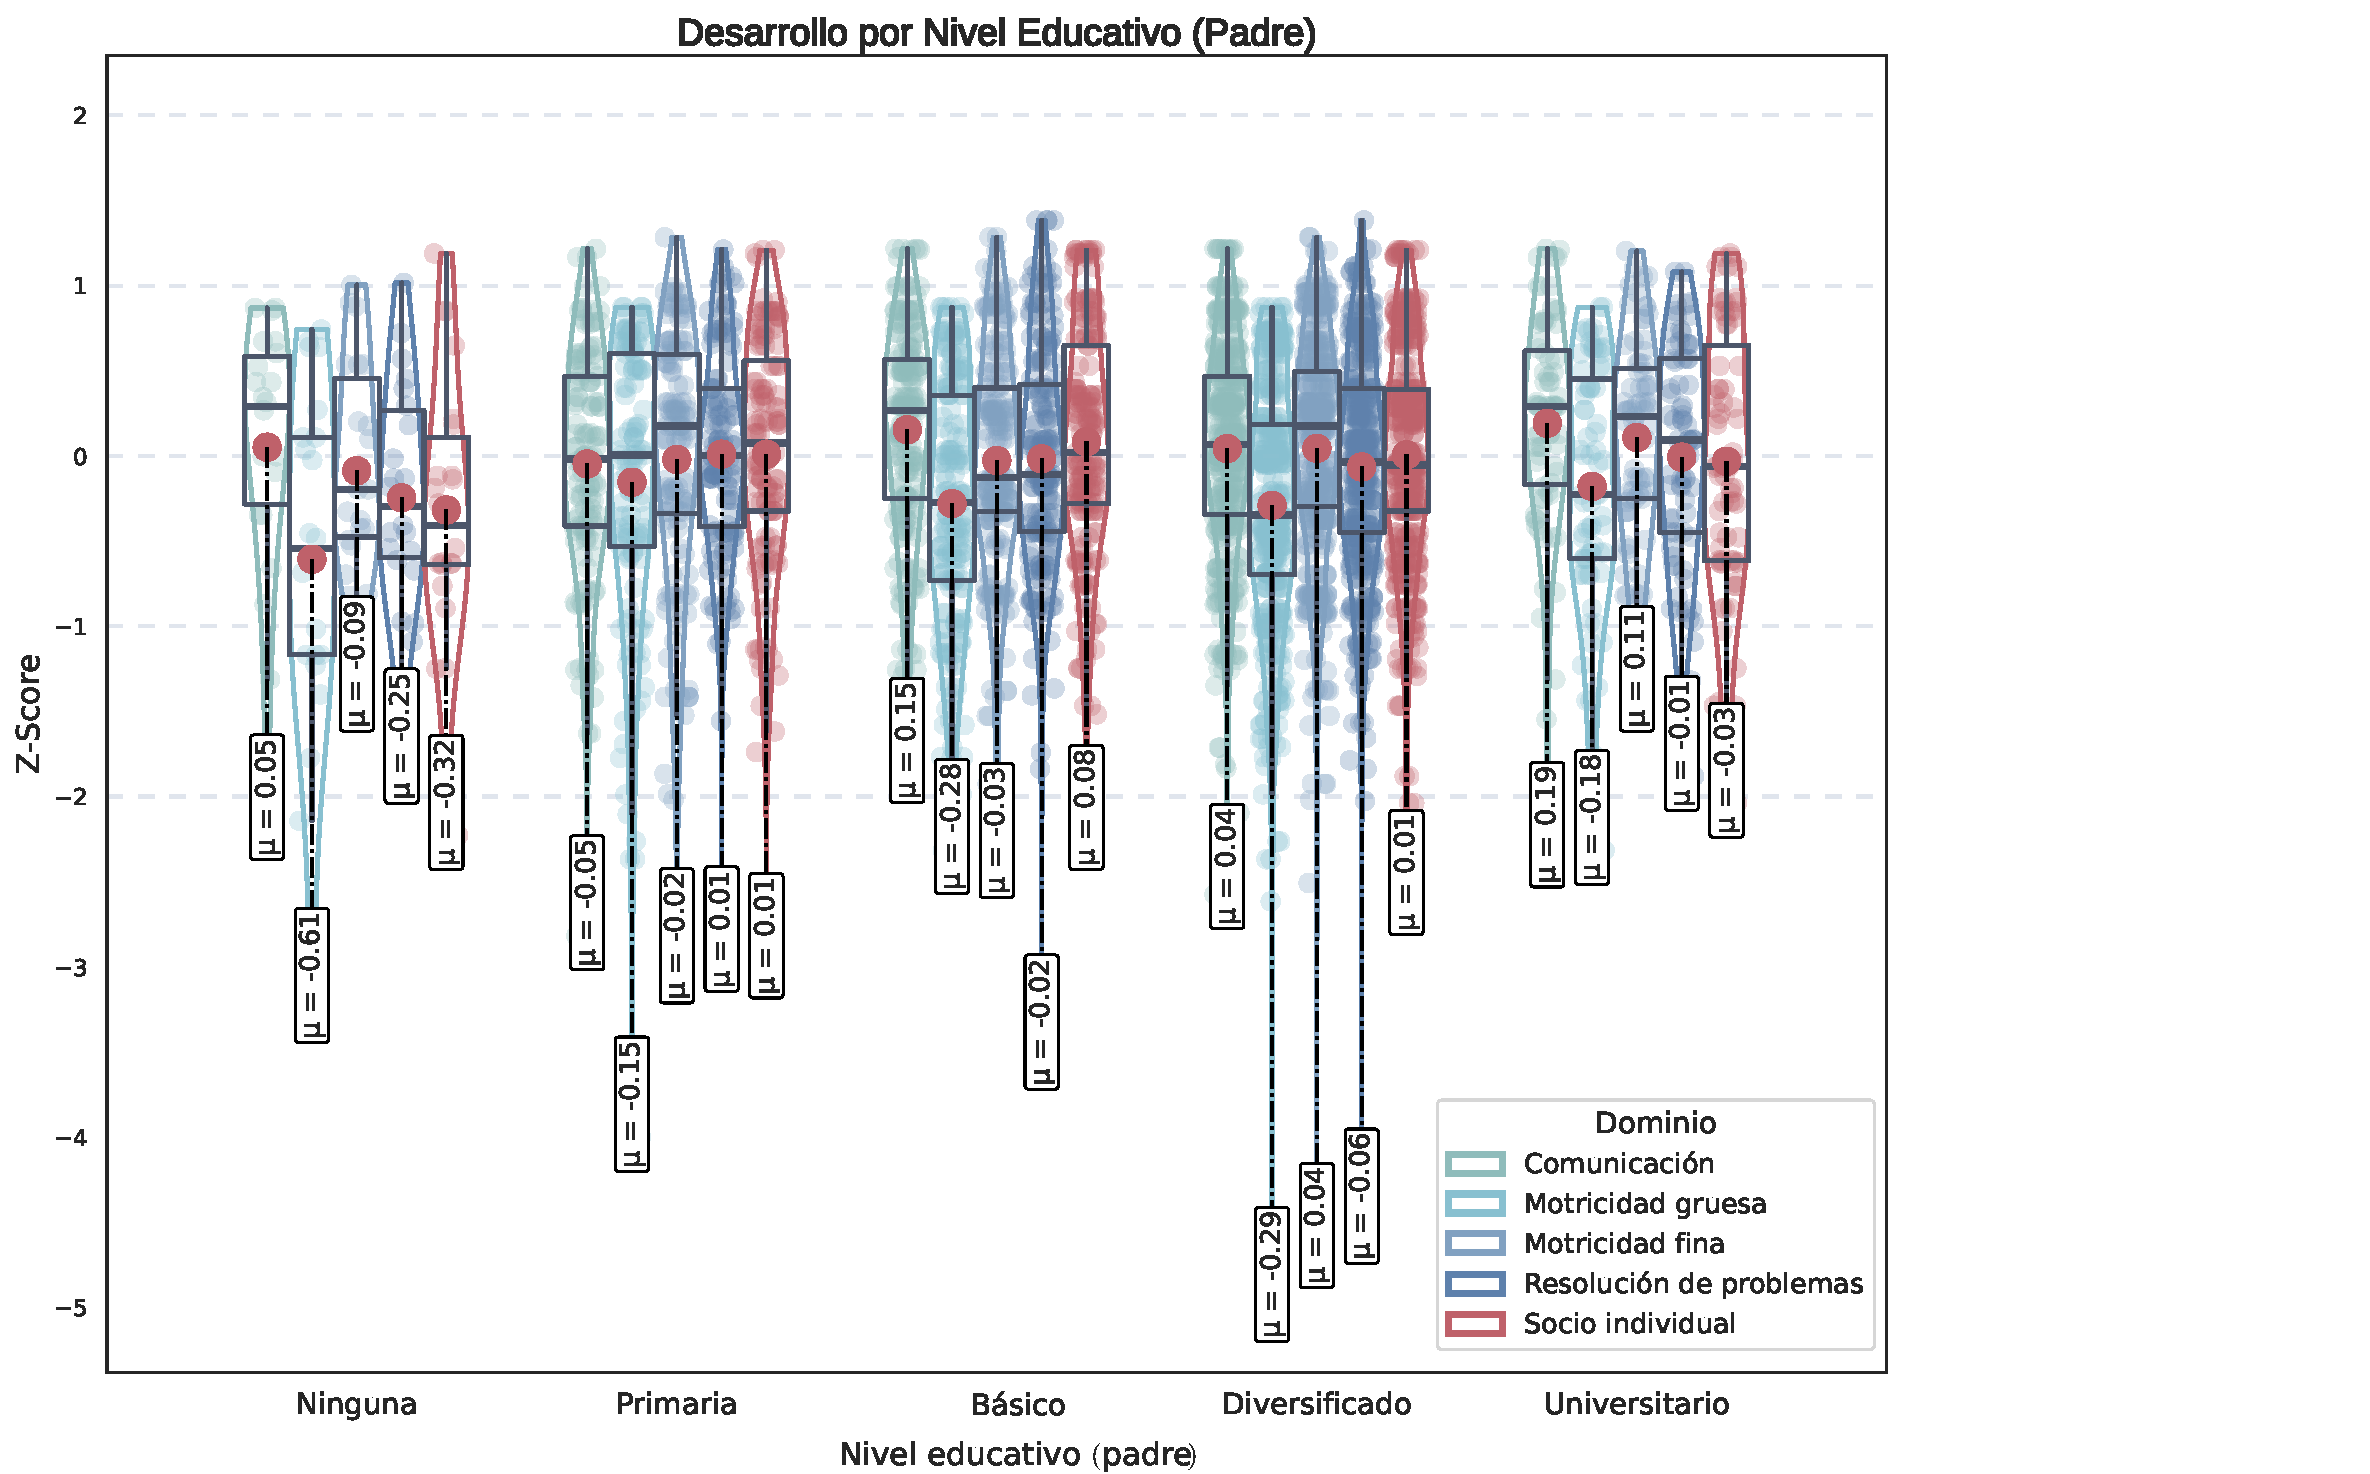
\includegraphics[width=1\textwidth]{violinplot_nivel_educativo_padre}
	\captionsetup{font=footnotesize}
	\caption{Desarrollo por nivel educativo (padre). Fuente: Cuadro \ref{tab:nivel_educativo_padre_desarrollo}}
    \label{fig:nivel_educativo_anova_padre}
\end{figure}

\begin{table}[htbp]
\centering
\caption{Asociación entre situación laboral del padre y riesgo en dominios del desarrollo}
\label{tab:situacion_laboral_padre_resumen_compacta}
\begin{threeparttable}
\begin{tblr}{
  width = 0.75\linewidth,
  colspec = {X[1.5,l]X[1.0,c]X[1.1,c]X[1.0,c]X[1.3,c]X[1.1,c]},
  row{1} = {font=\bfseries, bg=gray!10},
  row{even} = {bg=gray!3},
  cells = {valign=m, font=\footnotesize},
  hline{1,2,Z} = {1pt},
  hline{3-Y} = {0.5pt, gray},
}
\textbf{Dominio} & \textbf{$\chi^2$} & \textbf{\textit{p}-valor} & \textbf{OR} & \textbf{IC 95\%} & \textbf{Significativo} \\
Comunicación          & 0.57   & 0.451     & --    & --            & No \\
Motricidad gruesa     & 8.00   & 0.005     & 1.78  & 1.21--2.62    & Sí \\
Motricidad fina       & 0.51   & 0.473     & --    & --            & No \\
Resolución de problemas & 0.09   & 0.767     & --    & --            & No \\
Socio-individual      & 1.80   & 0.180     & --    & --            & No \\
\end{tblr}
\begin{tablenotes}
\footnotesize
\item \textbf{Método:} Prueba Chi-cuadrado.
\item \textbf{Nota:} Dominios con asociaciones significativas: 1/5. El grupo de niños con padre que no trabaja tiene mayor riesgo en el dominio de motricidad gruesa (OR = 1.78).
\end{tablenotes}
\end{threeparttable}
\end{table}

\begin{table}[htbp]
\centering
\caption{Asociación entre el total de hermanos y riesgo en dominios del desarrollo}
\label{tab:total_hermanos_desarrollo}
\begin{threeparttable}
\begin{tblr}{
  width = 0.97\linewidth,
  colspec = {X[1.3,l]X[0.8,c]X[1.0,c]X[1.0,c]X[1.0,c]X[0.7,c]},
  row{1} = {font=\bfseries, bg=gray!10},
  row{even} = {bg=gray!3},
  cells = {valign=m, font=\footnotesize},
  hline{1,2,Z} = {1pt},
  hline{3-Y} = {0.5pt, gray},
}
\textbf{Dominio} & \textbf{F/W} & \textbf{\textit{p}-valor} & \textbf{Significativo} & \textbf{Método} & \textbf{N} \\
Comunicación          & 5.71   & $<$0.001  & Sí  & ANOVA         & 1725 \\
Motricidad gruesa     & 2.44   & 0.063     & No  & ANOVA         & 1725 \\
Motricidad fina       & 3.70   & 0.011     & Sí  & ANOVA         & 1725 \\
Resolución de problemas & 0.78 & 0.504     & No  & ANOVA         & 1725 \\
Socio-individual      & 2.91   & 0.034     & Sí  & ANOVA         & 1725 \\
\end{tblr}
\begin{tablenotes}
\footnotesize
\item \textbf{Nota:} En dominios de comunicación y socio-individual, el grupo de
>3 hermanos muestra mayor riesgo y menor desempeño en puntajes Z. En motricidad
fina, los grupos extremos (0 y >3 hermanos) presentan menor media Z que grupos
de 1 y 2 hermanos.
\end{tablenotes}
\end{threeparttable}
\end{table}

\begin{table}[htbp]
\centering
\caption{Asociación entre el orden al nacer del niño y riesgo en dominios del desarrollo}
\label{tab:posicion_hermanos_desarrollo}
\begin{threeparttable}
\begin{tblr}{
  width = 0.97\linewidth,
  colspec = {X[1.3,l]X[0.8,c]X[1.0,c]X[1.0,c]X[1.0,c]X[0.7,c]},
  row{1} = {font=\bfseries, bg=gray!10},
  row{even} = {bg=gray!3},
  cells = {valign=m, font=\footnotesize},
  hline{1,2,Z} = {1pt},
  hline{3-Y} = {0.5pt, gray},
}
\textbf{Dominio} & \textbf{F/W} & \textbf{\textit{p}-valor} & \textbf{Significativo} & \textbf{Método} & \textbf{N} \\
Comunicación          & 3.27   & 0.011     & Sí  & ANOVA         & 1725 \\
Motricidad gruesa     & 1.25   & 0.290     & No  & ANOVA         & 1725 \\
Motricidad fina       & 2.80   & 0.025     & Sí  & ANOVA         & 1725 \\
Resolución de problemas & 0.76 & 0.554     & No  & ANOVA         & 1725 \\
Socio-individual      & 0.73   & 0.571     & No  & ANOVA         & 1725 \\
\end{tblr}
\begin{tablenotes}
\footnotesize
\item \textbf{Nota:} El cuarto niño es el grupo más afectado en el dominio de
comunicación (mayor riesgo, menor media Z). El grupo de primogénitos es el que
presenta mayor riesgo en motricidad fina. El resto de dominios no presentan
resultados significativos.
\end{tablenotes}
\end{threeparttable}
\end{table}

\begin{table}[htbp]
\centering
\caption{Asociación entre tipo de parto y riesgo en dominios del desarrollo}
\label{tab:tipo_parto_desarrollo}
\begin{threeparttable}
\begin{tblr}{
  width = 0.85\linewidth,
  colspec = {X[1.4,l]X[0.8,c]X[1.0,c]X[1.0,c]X[1.0,c]X[0.7,c]},
  row{1} = {font=\bfseries, bg=gray!10},
  row{even} = {bg=gray!3},
  cells = {valign=m, font=\footnotesize},
  hline{1,2,Z} = {1pt},
  hline{3-Y} = {0.5pt, gray},
}
\textbf{Dominio} & \textbf{F/W} & \textbf{\textit{p}-valor} & \textbf{Significativo} & \textbf{Método} & \textbf{N} \\
Comunicación          & 2.26   & 0.106     & No  & Welch's ANOVA & 1725 \\
Motricidad gruesa     & 0.04   & 0.956     & No  & Welch's ANOVA & 1725 \\
Motricidad fina       & 0.77   & 0.462     & No  & ANOVA         & 1725 \\
Resolución de problemas & 0.19 & 0.828     & No  & Welch's ANOVA & 1725 \\
Socio-individual      & 0.82   & 0.439     & No  & Welch's ANOVA & 1725 \\
\end{tblr}
\begin{tablenotes}
\footnotesize
\item \textbf{Nota:} No se encontraron asociaciones significativas entre el tipo de parto y el riesgo en ningún dominio del desarrollo infantil (\textit{p} $>$ 0.05 en todos los casos).
\end{tablenotes}
\end{threeparttable}
\end{table}

\begin{table}[htbp]
\centering
\caption{Asociación entre servicio de asistencia al parto y riesgo en dominios del desarrollo}
\label{tab:servicio_asistencia_parto_desarrollo}
\begin{threeparttable}
\begin{tblr}{
  width = 0.85\linewidth,
  colspec = {X[1.4,l]X[0.8,c]X[1.0,c]X[1.0,c]X[1.0,c]X[0.7,c]},
  row{1} = {font=\bfseries, bg=gray!10},
  row{even} = {bg=gray!3},
  cells = {valign=m, font=\footnotesize},
  hline{1,2,Z} = {1pt},
  hline{3-Y} = {0.5pt, gray},
}
\textbf{Dominio} & \textbf{F/W} & \textbf{\textit{p}-valor} & \textbf{Significativo} & \textbf{Método} & \textbf{N} \\
Comunicación          & 1.65   & 0.159     & No  & ANOVA         & 1725 \\
Motricidad gruesa     & 1.32   & 0.262     & No  & ANOVA         & 1725 \\
Motricidad fina       & 0.69   & 0.598     & No  & ANOVA         & 1725 \\
Resolución de problemas & 0.73 & 0.570     & No  & ANOVA         & 1725 \\
Socio-individual      & 2.41   & 0.072     & No  & Welch's ANOVA & 1725 \\
\end{tblr}
\begin{tablenotes}
\footnotesize
\item \textbf{Nota:} No se encontraron asociaciones significativas entre el servicio de asistencia al parto y el riesgo en ningún dominio del desarrollo infantil (\textit{p} $>$ 0.05 en todos los casos).
\end{tablenotes}
\end{threeparttable}
\end{table}

\begin{table}[htbp]
\centering
\caption{Asociación entre antecedentes de retardo de crecimiento y riesgo en dominios del desarrollo}
\label{tab:retardo_crecimiento_chi2_compacta}
\begin{threeparttable}
\begin{tblr}{
  width = 0.75\linewidth,
  colspec = {X[1.5,l]X[1.0,c]X[1.1,c]X[1.0,c]X[1.3,c]X[1.1,c]},
  row{1} = {font=\bfseries, bg=gray!10},
  row{even} = {bg=gray!3},
  cells = {valign=m, font=\footnotesize},
  hline{1,2,Z} = {1pt},
  hline{3-Y} = {0.5pt, gray},
}
\textbf{Dominio} & \textbf{$\chi^2$} & \textbf{\textit{p}-valor} & \textbf{OR} & \textbf{IC 95\%} & \textbf{Significativo} \\
Comunicación          & 0.81   & 0.369     & --    & --            & No \\
Motricidad gruesa     & 4.60   & 0.032     & 0.66  & 0.46--0.95    & Sí \\
Motricidad fina       & 3.69   & 0.055     & --    & --            & No \\
Resolución de problemas & 0.43   & 0.510     & --    & --            & No \\
Socio-individual      & 8.01   & 0.005     & 0.49  & 0.31--0.79    & Sí \\
\end{tblr}
\begin{tablenotes}
\footnotesize
\item \textbf{Método:} Prueba Chi-cuadrado.
\item \textbf{Nota:} El retardo de crecimiento afecta significativamente 2 de 5 dominios del neurodesarrollo, con mayor impacto en Motricidad gruesa (OR = 0.66).
\end{tablenotes}
\end{threeparttable}
\end{table}

\begin{table}[htbp]
\centering
\caption{Asociación entre antecedente de desnutrición aguda y riesgo en dominios del desarrollo}
\label{tab:desnutricion_aguda_resumen_compacta}
\begin{threeparttable}
\begin{tblr}{
  width = 0.75\linewidth,
  colspec = {X[1.5,l]X[1.0,c]X[1.1,c]X[1.0,c]X[1.3,c]X[1.1,c]},
  row{1} = {font=\bfseries, bg=gray!10},
  row{even} = {bg=gray!3},
  cells = {valign=m, font=\footnotesize},
  hline{1,2,Z} = {1pt},
  hline{3-Y} = {0.5pt, gray},
}
\textbf{Dominio} & \textbf{$\chi^2$} & \textbf{\textit{p}-valor} & \textbf{OR} & \textbf{IC 95\%} & \textbf{Significativo} \\
Comunicación          & 1.50   & 0.221     & --    & --            & No \\
Motricidad gruesa     & 0.90   & 0.342     & --    & --            & No \\
Motricidad fina       & 1.00   & 0.316     & --    & --            & No \\
Resolución de problemas & 1.30   & 0.254     & --    & --            & No \\
Socio-individual      & 4.05   & 0.044     & 1.97  & 1.07--3.64    & Sí \\
\end{tblr}
\begin{tablenotes}
\footnotesize
\item \textbf{Método:} Prueba Chi-cuadrado.
\item \textbf{Nota:} El antecedente de desnutrición aguda se asocia significativamente a riesgo en el dominio Socio-individual (OR = 1.97).
\end{tablenotes}
\end{threeparttable}
\end{table}

\begin{table}[htbp]
\centering
\caption{Asociación entre hospitalización neonatal y riesgo en dominios del desarrollo}
\label{tab:hospitalizado_neonatal_resumen}
\begin{threeparttable}
\begin{tblr}{
  width = 0.8\linewidth,
  colspec = {X[1.5,l]X[1, c]X[1, c]X[1, c]X[1.2, c]X[1, c]},
  row{1} = {font=\bfseries, bg=gray!10},
  row{even} = {bg=gray!3},
  cells = {valign=m, font=\footnotesize},
  hline{1,2,Z} = {1pt},
  hline{3-Y} = {0.5pt, gray},
}
\textbf{Dominio} & \textbf{Chi-cuadrado} & \textbf{\textit{p}-valor} & \textbf{OR} & \textbf{IC 95\%} & \textbf{Significativo} \\
Comunicación          & 0.00  & 1.000  & -- & -- & No \\
Motricidad gruesa     & 1.39  & 0.238  & -- & -- & No \\
Motricidad fina       & 3.18  & 0.075  & -- & -- & No \\
Resolución de problemas & 0.79 & 0.375  & -- & -- & No \\
Socio-individual      & 2.47  & 0.116  & -- & -- & No \\
\end{tblr}
\begin{tablenotes}
\footnotesize
\item \textbf{Nota:} Esta variable no muestra asociaciones significativas con el
neurodesarrollo infantil en ningún dominio.
\end{tablenotes}
\end{threeparttable}
\end{table}

\begin{table}[htbp]
\centering
\caption{Asociación entre hospitalización en la infancia y riesgo en dominios del desarrollo}
\label{tab:hospitalizado_infancia_resumen}
\begin{threeparttable}
\begin{tblr}{
  width = 0.8\linewidth,
  colspec = {X[1.5,l]X[1, c]X[1, c]X[1, c]X[1.2, c]X[1, c]},
  row{1} = {font=\bfseries, bg=gray!10},
  row{even} = {bg=gray!3},
  cells = {valign=m, font=\footnotesize},
  hline{1,2,Z} = {1pt},
  hline{3-Y} = {0.5pt, gray},
}
\textbf{Dominio} & \textbf{Chi-cuadrado} & \textbf{\textit{p}-valor} & \textbf{OR} & \textbf{IC 95\%} & \textbf{Significativo} \\
Comunicación          & 0.44  & 0.509  & -- & -- & No \\
Motricidad gruesa     & 2.81  & 0.094  & -- & -- & No \\
Motricidad fina       & 1.46  & 0.227  & -- & -- & No \\
Resolución de problemas & 0.60 & 0.437  & -- & -- & No \\
Socio-individual      & 1.36  & 0.243  & -- & -- & No \\
\end{tblr}
\begin{tablenotes}
\footnotesize
\item \textbf{Nota:} Esta variable no muestra asociaciones significativas con el
neurodesarrollo infantil en ningún dominio.
\end{tablenotes}
\end{threeparttable}
\end{table}

\begin{table}[htbp]
\centering
\caption{Asociación entre las horas de exposición a pantallas y riesgo en dominios del desarrollo}
\label{tab:horas_exposicion_pantallas_desarrollo}
\begin{threeparttable}
\begin{tblr}{
  width = 0.97\linewidth,
  colspec = {X[1.3,l]X[0.8,c]X[1.0,c]X[1.0,c]X[1.0,c]X[0.7,c]},
  row{1} = {font=\bfseries, bg=gray!10},
  row{even} = {bg=gray!3},
  cells = {valign=m, font=\footnotesize},
  hline{1,2,Z} = {1pt},
  hline{3-Y} = {0.5pt, gray},
}
\textbf{Dominio} & \textbf{F/W} & \textbf{\textit{p}-valor} & \textbf{Significativo} & \textbf{Método} & \textbf{N} \\
Comunicación          & 3.79   & 0.010     & Sí  & ANOVA         & 1725 \\
Motricidad gruesa     & 2.62   & 0.049     & Sí  & ANOVA         & 1725 \\
Motricidad fina       & 2.99   & 0.030     & Sí  & ANOVA         & 1725 \\
Resolución de problemas & 3.75 & 0.011     & Sí  & ANOVA         & 1725 \\
Socio-individual      & 4.33   & 0.005     & Sí  & ANOVA         & 1725 \\
\end{tblr}
\begin{tablenotes}
\footnotesize
\item En todos los dominios, se observa una tendencia a mayor riesgo en el
desarrollo con mayor número de horas de exposición a pantallas. Los grupos más
afectados son los de $\geq$ 6 horas en motricidad fina y 4-5 horas en
socio-individual.
\end{tablenotes}
\end{threeparttable}
\end{table}

\begin{table}[htbp]
\centering
\caption{Asociación entre las horas de juego con cuidador y riesgo en dominios del desarrollo}
\label{tab:horas_juego_cuidador_desarrollo}
\begin{threeparttable}
\begin{tblr}{
  width = 0.97\linewidth,
  colspec = {X[1.3,l]X[0.8,c]X[1.0,c]X[1.0,c]X[1.0,c]X[0.7,c]},
  row{1} = {font=\bfseries, bg=gray!10},
  row{even} = {bg=gray!3},
  cells = {valign=m, font=\footnotesize},
  hline{1,2,Z} = {1pt},
  hline{3-Y} = {0.5pt, gray},
}
\textbf{Dominio} & \textbf{F/W} & \textbf{\textit{p}-valor} & \textbf{Significativo} & \textbf{Método} & \textbf{N} \\
Comunicación          & 1.19   & 0.314     & No  & Welch's ANOVA & 1725 \\
Motricidad gruesa     & 3.05   & 0.028     & Sí  & ANOVA         & 1725 \\
Motricidad fina       & 2.57   & 0.053     & No  & ANOVA         & 1725 \\
Resolución de problemas & 6.49 & $<$0.001  & Sí  & ANOVA         & 1725 \\
Socio-individual      & 0.23   & 0.878     & No  & ANOVA         & 1725 \\
\end{tblr}
\begin{tablenotes}
\footnotesize
\item \textbf{Nota:} El grupo con menos horas de juego (0-1 horas) es el más
afectado en motricidad gruesa y resolución de problemas, mostrando mayor riesgo
y menores puntuaciones Z.
\end{tablenotes}
\end{threeparttable}
\end{table}

\chapter{Discusión y análisis}
Este estudio tuvo como objetivo establecer la asociación entre factores 
sociodemográficos, económicos, familiares y médicos con el riesgo en el 
neurodesarrollo en niños menores de 5 años que asisten a servicios de atención 
primaria en el distrito de Quetzaltenango, mediante evaluaciones con el
Cuestionario Edades y Etapas 3. Los resultados obtenidos fueron sometidos a
pruebas de  normalidad de Kolmogorov-Smirnov, confirmando distribuciones
aproximadamente  normales para todos los dominios del desarrollo 
(Cuadro~\ref{tab:estadisticas_z_scores}). Posteriormente se realizó un análisis 
descriptivo y un análisis inferencial utilizando chi-cuadrado y ANOVA para
identificar grupos de riesgo y su significancia estadística.

La muestra de 1,725 niños menores de 5 años mostró una distribución por sexo 
con predominancia masculina (53.45\%) sobre femenina (46.55\%), como se 
observa en el Cuadro~\ref{tab:resultado1}. La distribución etaria reveló mayor 
concentración en los grupos de 7-12 meses (19.7\%), lo que refleja las
características de la población que acude a servicios de 
atención primaria para controles de crecimiento y vacunación. 

En cuanto a la edad gestacional al nacer, el 89.5\% fueron nacimientos a 
término, con un 10.5\% de prematuridad en diferentes grados 
(Cuadro~\ref{tab:eg}). Similar a estudios en Guatemala que estiman 12.6\% de partos pretérmino \cite{Pusdekar2020}.

La distribución étnica mostró 57.04\% de población no indígena y 42.96\% 
indígena, con marcada concentración de población indígena en área rural 
(71.2\%), mientras que el 85.1\% de la muestra total reside en área urbana 
(Cuadro~\ref{tab:etnia-residencia}). Esta distribución refleja las 
características demográficas del departamento de Quetzaltenango y es 
fundamental para interpretar los resultados del neurodesarrollo considerando 
diferencias demográficas y socioeconómicas.

Las características familiares revelaron que las edades parentales se 
concentraron entre 25-29 años (madres 32.0\%, padres 27.3\%), con edad 
promedio materna de 27.85 años y paterna de 30.42 años 
(Cuadro~\ref{tab:edad_padres}). El nivel educativo predominante fue 
diversificado tanto en madres (40.90\%) como en padres (48.50\%), 
observándose mayor proporción de educación superior en padres 
(Cuadro~\ref{tab:escolaridad}).

Respecto al empleo, el 50.0\% de madres no trabajaban, mientras que el 63.01\% 
de padres tenían empleo formal (Cuadro~\ref{tab:empleo}). Estas diferencias 
significativas en patrones de empleo por género ($\chi^2 = 1089.2$, 
$p < 0.001$) reflejan roles tradicionales de género en la región.

El acceso a servicios básicos fue favorable: 90.55\% con agua potable, 93.62\% 
con saneamiento adecuado, 100\% con electricidad y 87.13\% con gas propano 
para cocinar (Cuadro~\ref{tab:servicios_basicos}). La composición familiar 
mostró predominio de hogares de 3-4 personas (43.54\%), con promedio de 1.21 
hermanos y 40.23\% de primogénitos (Cuadro~\ref{tab:composicion_familiar}).

La cobertura prenatal fue adecuada con promedio de 6.70 controles prenatales, 
94.55\% con acceso a ultrasonido obstétrico, 88.17\% consumieron vitaminas
prenatales en el primer trimestre del embarazo y 92.93\% consumieron vitaminas
prenatales durante el resto del embarazo (Cuadro~\ref{tab:cuidados_prenatales}). 
La mayoría de partos fueron atendidos en hospitales públicos (64.7\%) con 
resolución por vía vaginal (59.0\%) (Figura~\ref{fig:parto}). Se encontraron mejores condiciones en la región comparado con resultados de la Encuesta Nacional de Salud Materno Infantil de 2014-2025 que reportaban menor suplementación con ácido fólico y menor calidad de atención antenatal \cite{Santos2025}.

Las principales causas de cesárea de emergencia fueron complicaciones del 
líquido amniótico (43.4\%), sufrimiento fetal (26.4\%) y preeclampsia (11.3\%) 
(Cuadro~\ref{tab:causas_cesarea}).

La lactancia materna exclusiva mostró tendencia decreciente con la edad: 72.7\% 
(0-6 meses), 55.6\% (6-12 meses) y 48.1\% (12-24 meses), con incremento 
correspondiente de lactancia mixta (Cuadro~\ref{tab:lactancia_periodos}). La 
suplementación con vitamina A disminuyó de 69.7\% (6-12 meses) a 53.9\% 
(18-24 meses) (Cuadro~\ref{tab:vitamina_a}), patrón similar para vitaminas y 
minerales espolvoreados (Cuadro~\ref{tab:vitaminas_minerales}). Esta 
disminución podría relacionarse con menor asistencia a servicios de salud a 
mayor edad del niño.

Los antecedentes nutricionales mostraron retardo de crecimiento en 11.1\% y 
desnutrición aguda en 5.9\% (Cuadro~\ref{tab:antecedentes_nutricionales}). 
Las hospitalizaciones fueron 12.0\% neonatales y 13.7\% en infancia 
(Cuadro~\ref{tab:hospitalizacion}), con ictericia neonatal (33.8\%) y neumonía 
(50.2\%) como principales causas respectivas 
(Cuadro~\ref{tab:causas_hospitalizacion}). La cobertura de vacunas en la alcanzó
94.9\% (Cuadro~\ref{tab:vacunacion}).

Los resultados del Cuestionario Edades y Etapas 3 revelaron desarrollo adecuado
en comunicación (94.4\%),  resolución de problemas (92.6\%), desarrollo
socio-individual (92.8\%),  motricidad fina (91.4\%) y motricidad gruesa
(83.3\%)  (Cuadro~\ref{tab:desarrollo_dominios}). La motricidad gruesa mostró
mayor  vulnerabilidad con 16.7\% en riesgo, confirmando los hallazgos del
análisis de puntajes Z donde este dominio presentó la media más baja (-0.269) 
(Cuadro~\ref{tab:estadisticas_z_scores}). Se encontraron menores porcentajes de riesgo en los diferentes dominios del desarrollo comparado con estudios anteriores en Guatemala que reportaban hasta 40\% de desarrollo en riesgo en el dominio de motricidad fina \cite{Angulo2023}.

La clasificación global del desarrollo mostró que 66.96\% de niños tienen 
desarrollo adecuado global, 33.04\% presentan riesgo en cualquier dominio y 
5.22\% alto riesgo (Cuadro~\ref{tab:desarrollo_global}). Se encontraron menores porcentajes de riesgo en cualquier dominio del neurodesarrollo comparado con estudios de Argentina (45\%) y Perú (38.7\%) pero mayores en relación a poblaciones de Cuba (21.5\%) y México (14.7\%)
\cite{GuadarramaCelaya2011,Kyerematen2014,CarlosOliva2020,RicardoGarcell2022}.

\section{Análisis de asociación de variables}
El análisis estratificado por edad reveló patrones distintivos de riesgo en el 
neurodesarrollo con alta significancia estadística ($p<0.001$). Los 8 meses 
emergieron como el período de mayor vulnerabilidad (OR = 3.78, IC 95\%: 
[2.29, 6.24]), con una prevalencia de riesgo global del 63.8\%. Esta edad 
concentra múltiples asociaciones significativas con los dominios del desarrollo
(Figura~\ref{fig:prevalencia_riesgo_asq3}).

En contraste, se identificaron edades con patrones protectores notables: 6 meses 
(OR = 0.317, IC 95\%: [0.18, 0.56]), 12 meses (OR = 0.396, IC 95\%: [0.25, 0.62]) 
y 27 meses (OR = 0.272, IC 95\%: [0.14, 0.52]). Estos períodos mostraron la 
menor prevalencia de riesgo entre todos los grupos evaluados
(Figura~\ref{fig:odds_ratio_asq3}).

Se identificaron períodos adicionales de riesgo elevado a los 4, 16, 18, 20, 24 
y 60 meses, donde los odds ratios superaron el valor de 2.0, con prevalencias 
de riesgo superiores al 45\%. Esta distribución temporal de riesgos sugiere 
períodos críticos que requieren monitoreo específico del neurodesarrollo.
Estos patrones de edad y riesgo en el neurodesarrollo se acercan a las
recomendaciones de la Academia Americana de Pediatría en su programa Bright
Futures que propone de tamizar a los 9, 18, y 30 meses de edad, así como monitorear el desarrollo a los 2, 4, 6, 12, 15, 24, 36, 48, 60 meses \cite{Lipkin2020}. 

El análisis de asociación reveló que el sexo del niño no mostró diferencias 
significativas en ningún dominio del desarrollo: comunicación 
($\chi^2 = 2.986$, $p = 0.225$), motricidad gruesa ($\chi^2 = 1.376$, 
$p = 0.503$), motricidad fina ($\chi^2 = 1.591$, $p = 0.451$), resolución 
de problemas ($\chi^2 = 1.957$, $p = 0.376$) y socio-individual 
($\chi^2 = 0.340$, $p = 0.844$) (Cuadro~\ref{tab:sexo_nino_desarrollo_chi2}), 
contrastando con estudios que exponen diferencias significativas en las que
el sexo masculino se asocia con mayor riesgo de trastornos del neurodesarrollo \cite{Sudry2024,Christensen2025,Peyre2019,Nishimura2016}.

Sin embargo, el grupo étnico mostró asociaciones significativas en resolución 
de problemas ($\chi^2 = 4.57$, $p = 0.033$, OR = 1.50, IC 95\%: 1.05-2.16) 
y desarrollo socio-individual ($\chi^2 = 4.90$, $p = 0.027$, OR = 1.53, 
IC 95\%: 1.06-2.21), con mayor riesgo en población indígena. Los dominios sin 
asociación significativa fueron: comunicación ($\chi^2 = 2.73$, $p = 0.098$), 
motricidad gruesa ($\chi^2 = 0.39$, $p = 0.533$) y motricidad fina 
($\chi^2 = 1.89$, $p = 0.169$) 
(Cuadro~\ref{tab:grupo_etnico_desarrollo_chi2_compacta}). Este hallazgo 
sugiere que las disparidades étnicas reflejan inequidades en oportunidades de
desarrollo, la misma observación se ha encontrado en comunidades de Australia, Canada, Nueva Zelanda, Estados Unidos, Brasil y Argentina
\cite{Lau2022,Hanly2020,Wehby2017}.

El área de residencia mostró asociaciones robustas con riesgo en cuatro 
dominios: comunicación ($\chi^2 = 8.70$, $p = 0.003$, OR = 2.09, 
IC 95\%: 1.30-3.36), motricidad gruesa ($\chi^2 = 12.62$, $p < 0.001$, 
OR = 1.79, IC 95\%: 1.31-2.46), resolución de problemas ($\chi^2 = 25.13$, 
$p < 0.001$, OR = 2.77, IC 95\%: 1.85-4.15) y socio-individual 
($\chi^2 = 15.06$, $p < 0.001$, OR = 2.31, IC 95\%: 1.52-3.51), todos con 
mayor riesgo en área rural. Solo motricidad fina no mostró asociación 
significativa ($\chi^2 = 1.73$, $p = 0.188$) 
(Cuadro~\ref{tab:area_residencia_desarrollo_chi2_compacta}). Esta asociación
refleja desventajas en la población rural de Quetzaltenango, lo que es consistente con estudios de Estados Unidos, India, China y Pakistán \cite{Zablotsky2020-tb,Chatterjee2020,Murthy2020,Wang2020,Avan2010}

El nivel educativo materno se asoció significativamente con todos los dominios 
del desarrollo: comunicación ($F = 5.96$, $p < 0.001$), motricidad gruesa 
($F = 6.29$, $p < 0.001$), motricidad fina ($F = 8.68$, $p < 0.001$), 
resolución de problemas ($F = 9.51$, $p < 0.001$) y socio-individual 
($F = 6.44$, $p < 0.001$), donde el grupo universitario mostró puntajes más 
altos y diferencias significativas con otros grupos, mientras que ``ninguna 
escolaridad'' presentó valores más bajos 
(Cuadro~\ref{tab:nivel_educativo_madre_desarrollo_anova}). Esto es consistente
con resultados de estudios longitudinales realizados en Francia, Singapur y Brasil que reportan menores puntajes en niños de madres con bajo nivel educativo \cite{Charkaluk2024,Lockhart2023,Yeleswarapu2025,Munhoz2022}, y mayores puntajes en todos los dominios en madres con mayor nivel educativo en artículos de Perú e Indonesia \cite{Handal2007,Hanifah2022}.


El nivel educativo 
paterno se asoció con comunicación ($F = 6.82$, $p < 0.001$) y socio-individual 
($F = 2.57$, $p = 0.036$), pero no con motricidad gruesa ($F = 1.88$, 
$p = 0.114$), motricidad fina ($F = 1.09$, $p = 0.359$) ni resolución de 
problemas ($F = 1.36$, $p = 0.247$) 
(Cuadro~\ref{tab:nivel_educativo_padre_desarrollo}). Esto se evidencia en países como Dinamarca, Noruega, y Estados Unidos \cite{Holstein2021,Torvik2020,Sauver2004}

La situación laboral paterna se asoció específicamente con motricidad gruesa 
($\chi^2 = 8.00$, $p = 0.005$, OR = 1.78, IC 95\%: 1.21-2.62), donde niños 
con padres desempleados presentaron mayor riesgo. Los otros dominios no 
mostraron asociación significativa: comunicación ($\chi^2 = 0.57$, $p = 0.451$), 
motricidad fina ($\chi^2 = 0.51$, $p = 0.473$), resolución de problemas 
($\chi^2 = 0.09$, $p = 0.767$) y socio-individual ($\chi^2 = 1.80$, 
$p = 0.180$) (Cuadro~\ref{tab:situacion_laboral_padre_resumen_compacta}). 
Este hallazgo puede reflejar el impacto de inestabilidad económica en 
acceso a recursos nutricionales que favorecen el desarrollo motor.

La situación laboral materna no se asoció significativamente con riesgos en los
dominios del desarrollo.

El estado civil del cuidador mostró asociaciones significativas en comunicación 
($F = 10.18$, $p < 0.001$), motricidad gruesa ($F = 5.03$, $p = 0.007$), 
resolución de problemas ($F = 6.12$, $p = 0.002$) y socio-individual 
($F = 3.88$, $p = 0.021$), donde niños de madres solteras presentaron 
menor desempeño. Solo motricidad fina no mostró asociación ($F = 1.60$, 
$p = 0.202$) (Cuadro~\ref{tab:estado_civil_cuidador_desarrollo}). El número 
de hermanos se asoció con comunicación ($F = 5.71$, $p < 0.001$), motricidad 
fina ($F = 3.70$, $p = 0.011$) y socio-individual ($F = 2.91$, $p = 0.034$), 
pero no con motricidad gruesa ($F = 2.44$, $p = 0.063$) ni resolución de 
problemas ($F = 0.78$, $p = 0.504$), donde familias con más de 3 hermanos 
mostraron mayor riesgo (Cuadro~\ref{tab:total_hermanos_desarrollo}).
Una revisión sistemática de la literatura encontró que los niños en núcleos
familiares de padres solteros tienen mayor riesgo de presentar TDAH
\cite{Claussen2022}.

El retardo de crecimiento se asoció con riesgo en motricidad gruesa
($\chi^2 = 4.60$, $p = 0.032$, OR = 0.66, IC 95\%: 0.46-0.95) y el dominio
socio-individual ($\chi^2 = 8.01$, $p = 0.005$, OR = 0.49, IC 95\%: 0.31-0.79),
pero no con dominios de comunicación ($\chi^2 = 0.81$, $p = 0.369$), motricidad
fina ($\chi^2 = 3.69$, $p = 0.055$) ni resolución de problemas ($\chi^2 = 0.43$, $p = 0.510$) 
(Cuadro~\ref{tab:retardo_crecimiento_chi2_compacta}). La desnutrición aguda 
se relacionó específicamente con riesgo en el desarrollo socio-individual
($\chi^2 = 4.05$, $p = 0.044$, OR = 1.97, IC 95\%: 1.07-3.64), pero no con otros
dominios:  comunicación ($\chi^2 = 1.50$, $p = 0.221$), motricidad gruesa 
($\chi^2 = 0.90$, $p = 0.342$), motricidad fina ($\chi^2 = 1.00$, $p = 0.316$) 
ni resolución de problemas ($\chi^2 = 1.30$, $p = 0.254$) 
(Cuadro~\ref{tab:desnutricion_aguda_resumen_compacta}), consistente con 
evidencia que sugiere que desnutrición tanto crónica como aguda afecta
competencias del desarrollo \cite{Babikako2022,Suryawan2021,vandenHeuvel2019}.

Las horas de exposición a pantallas (televisor, tablet, móvil) se asociaron
significativamente con riesgo en todos los dominios del desarrollo: comunicación
($F = 3.79$, $p = 0.010$), motricidad gruesa ($F = 2.62$, $p = 0.049$),
motricidad fina ($F = 2.99$, $p = 0.030$), resolución de problemas ($F = 3.75$,
$p = 0.011$) y  socio-individual ($F = 4.33$, $p = 0.005$), observándose mayor
riesgo con mayor exposición (Cuadro~\ref{tab:horas_exposicion_pantallas_desarrollo}). La literatura propone un modelo de disrupción de neurotransmisores como la acetilcolina, glutamato, serotonina como el mecanismo de aumento de
riesgo de trastornos del neurodesarrollo, el tiempo en pantalla se asocia a
déficit de atención, trastornos del habla y lenguaje, y si la exposición
es temprana puede asociarse con trastorno del espectro autista, aunque se
propone que actividades al aire libre reducen este riesgo \cite{Priyadarshini2025,Zehra2025,Hill2024,Sarfraz2023,Amorim2023,Sugiyama2023,Goswami2023,Jourdren2023}.

Las horas de juego que el cuidador le dedica al niño se asociaron con riesgos en
dominios de motricidad gruesa ($F = 3.05$, $p = 0.028$) y resolución de
problemas ($F = 6.49$, $p < 0.001$), pero no con comunicación ($F = 1.19$,
$p = 0.314$), motricidad fina ($F = 2.57$, $p = 0.053$) ni socio-individual
($F = 0.23$, $p = 0.878$), donde el grupo con menos horas (0-1) mostró mayor
riesgo (Cuadro~\ref{tab:horas_juego_cuidador_desarrollo}). Las interacciones entre cuidador y niño se asocian con mejores desenlaces del desarrollo, y son factores protectores de desarrollo cognitivo y conductual en infantes de alto riesgo de presentar trastornos del neurodesarrollo \cite{Jaffee2007,Isaev2023,Schneider2022}

\subsection{Factores sin asociación significativa}

Diversos factores no mostraron asociación significativa con el neurodesarrollo: 
edad materna y paterna ($p > 0.05$ en todos los dominios), total de personas en
el hogar ($p > 0.05$ en todos los dominios), número de controles prenatales
($p > 0.05$ en todos los dominios), vitaminas prenatales 
($p > 0.05$ en todos los dominios), 
tipo de parto ($p > 0.05$ en todos los dominios) 
(Cuadro~\ref{tab:tipo_parto_desarrollo}), servicio de asistencia al parto 
($p > 0.05$ en todos los dominios) 
(Cuadro~\ref{tab:servicio_asistencia_parto_desarrollo}), y antecedente de
hospitalización neonatal e infantil ($p > 0.05$ en todos los dominios) 
(Cuadros~\ref{tab:hospitalizado_neonatal_resumen} y 
\ref{tab:hospitalizado_infancia_resumen}). El acceso a seguridad social tampoco
mostró asociación significativa con riesgo en el neurodesarrollo ($p > 0.05$ en
todos los dominios). 

Este estudio presenta limitaciones inherentes al diseño transversal que impide 
establecer relaciones causales. La muestra, aunque representativa de la
población que acude a servicios de atención primaria, puede no reflejar
completamente características de la población general. La posible presencia de
factores de confusión no medidos, como calidad de interacción entre el cuidador
y el niño o condiciones médicas no diagnosticadas, o antecedentes médicos
erróneos podría influir en resultados observados.

\newpage

\chapter{Conclusiones}

\begin{enumerate}
\item
En el análisis de patrones de riesgo por edad se encontró que los 8 meses
constituyen el período con mayor prevalencia de riesgo del 63.8\% (OR = 3.78),
en contraste, las edades de 6 meses (OR = 0.317), 12 meses
(OR = 0.396) y 27 meses (OR = 0.272) mostraron patrones protectores,
indicando períodos de menor  en el desarrollo. Otras edades con alto
riesgo incluyen 4, 16, 18, 20, 24 y 60 meses, todas con prevalencia superior
al 45\%, evidenciando momentos críticos adicionales que requieren vigilancia
específica.

\item
Respecto a patrones de riesgo por dominios del neurodesarrollo,
la motricidad gruesa fue el área más afectada (16.7\%), seguida por motricidad
fina (8.6\%), desarrollo socio-individual (7.2\%), resolución de problemas
(7.4\%) y comunicación (5.6\%), en el total de la población.

\item
Los factores sociodemográficos mostraron asociaciones significativas con el
riesgo en el neurodesarrollo. La etnia indígena presentó 1.50 veces mayor
riesgo en resolución de problemas y 1.53 en desarrollo socio-individual. La
residencia rural se asoció con riesgo elevado en comunicación (OR = 2.09),
motricidad gruesa (OR = 1.79), resolución de problemas (OR = 2.77) y
desarrollo socio-individual (OR = 2.31), evidenciando las disparidades
territoriales en oportunidades de desarrollo.

En cuanto a factores familiares, el nivel educativo materno bajo fue el
factor más consistente, afectando todos los dominios del desarrollo
($p < 0.001$). El nivel educativo paterno bajo se asoció con comunicación
($p < 0.001$) y desarrollo socio-individual ($p = 0.036$). El desempleo
paterno mostró asociación específica con riesgo en motricidad gruesa
(OR = 1.78). Respecto a la estructura familiar, los primogénitos presentaron
mayor riesgo en motricidad fina.

Los factores ambientales también demostraron influencia significativa. El
tiempo de exposición prolongada a pantallas electrónicas mostró asociación
con riesgo en todos los dominios del desarrollo ($p < 0.05$), evidenciando
que a mayor tiempo de exposición, mayor riesgo de alteraciones en el
neurodesarrollo. En contraste, las horas de juego entre cuidadores y niños
demostraron ser un factor protector significativo, especialmente para
motricidad gruesa ($p = 0.028$) y resolución de problemas ($p < 0.001$),
confirmando la importancia de la interacción social directa para el
desarrollo óptimo.

\item La atención prenatal, incluyendo número de controles y suplementación,
no mostró asociaciones significativas con el riesgo en el neurodesarrollo
($p > 0.05$). Sin embargo, los factores nutricionales postnatales sí
evidenciaron asociaciones importantes. El retardo de crecimiento, presente en
11.1\% de la muestra, incremento el riesgo en motricidad gruesa (OR = 0.66)
y desarrollo socio-individual (OR = 0.49). La desnutrición aguda, con
prevalencia de 5.9\%, se asoció específicamente con riesgo en desarrollo
socio-individual (OR = 1.97). Otros factores médicos como edad gestacional,
tipo de parto y lugar de atención del parto no mostraron relación con el
riesgo en el neurodesarrollo, sugiriendo que los determinantes sociales
prevalecen sobre los factores biológicos en el contexto estudiado.

\item Este estudio evidenció que el riesgo en el neurodesarrollo infantil en
Quetzaltenango está determinado por múltiples factores interrelacionados,
destacando la edad crítica de 8 meses, el predominio de riesgo en motricidad
gruesa y la influencia significativa de determinantes sociales como etnia
indígena, residencia rural y nivel educativo parental principalmente el materno.
La exposición prolongada a pantallas representa un factor de riesgo evidente,
mientras que el tiempo de juego cuidador-niño actúa como factor protector.
Los hallazgos resaltan la necesidad de implementar estrategias preventivas
enfocadas en los períodos críticos identificados, priorizando poblaciones
vulnerables y promoviendo interacciones positivas entre cuidadores y niños
en lugar de la exposición a dispositivos electrónicos.
\end{enumerate}

\newpage

\section{Recomendaciones}

\subsection*{A las autoridades de salud}
\begin{enumerate}
\item Incorporar programas de tamizaje del neurodesarrollo infantil en 
servicios de primer y segundo nivel de atención.

\item Modificar el carné del niño y de la niña para incluir una sección 
específica de seguimiento de resultados del tamizaje del neurodesarrollo.

\item Implementar herramientas validadas como los Cuestionarios Edades y 
Etapas 3 (ASQ-3) o las Escalas Globales para el Desarrollo Temprano de la 
Organización Mundial de la Salud.

\item Priorizar el tamizaje intensivo a los 8 meses e incorporar el 
monitoreo en edades que coincidan con los períodos de vacunación (2, 4, 6, 
12, 18 y 48 meses).

\item Crear sistemas de referencia y contrarreferencia entre niveles de 
atención para casos con riesgo identificado en el tamizaje.

\item Destinar presupuesto específico para capacitación continua del 
personal de salud en aplicación e interpretación de herramientas de 
tamizaje.
\end{enumerate}

\subsection*{Al personal de salud}
\begin{enumerate}
\item Promover la importancia del tamizaje del neurodesarrollo infantil en 
la consulta de niño sano, especialmente a los 8 meses de edad.

\item Informar a los padres sobre actividades específicas de estimulación 
temprana e interacciones positivas cuidador-niño.

\item Elaborar charlas educativas sobre la importancia de los primeros mil 
días para el desarrollo infantil.

\item Utilizar material promocional de UNICEF y OMS para empoderar a los 
padres en el acceso a información sobre estimulación temprana.

\item Enfatizar en las consultas los riesgos de la exposición temprana y 
prolongada a dispositivos electrónicos en menores de 5 años.
\end{enumerate}

\subsection*{A los padres de familia}
\begin{enumerate}
\item Realizar actividades diarias de estimulación temprana estructuradas de acuerdo a la edad del niño:
\begin{itemize}
    \item 10-15 minutos de ejercicios de motricidad gruesa
    \item 10 minutos de estimulación del lenguaje con interacción responsiva
    \item 10 minutos de actividades de motricidad fina
\end{itemize}

\item Evitar la exposición temprana y prolongada de niños menores de 
5 años a pantallas de dispositivos electrónicos (televisores, tablets, 
teléfonos móviles), siguiendo las recomendaciones de la Academia Americana 
de Pediatría.

\item Promover el juego activo e interacciones directas entre 
cuidadores y niños como alternativa al uso de medios electrónicos, 
priorizando actividades que estimulen el desarrollo integral.

\item Permitir espacios de juego con otros niños para fortalecer 
habilidades socio-individuales y de comunicación.
\end{enumerate}

\subsection*{A las autoridades educativas}
\begin{enumerate}
\item Crear centros de desarrollo infantil temprano en comunidades rurales 
e indígenas con mayor vulnerabilidad.

\item Capacitar a maestros de educación inicial en identificación temprana 
de retrasos del desarrollo y uso de herramientas de tamizaje.

\item Desarrollar material educativo culturalmente apropiado sobre 
estimulación temprana para la población.
\end{enumerate}

\subsection*{A las autoridades departamentales}
\begin{enumerate}
\item Crear programas de estimulación temprana en coordinación 
con el sistema de salud, priorizando comunidades rurales.

\item Establecer centros comunitarios de desarrollo infantil en áreas 
rurales con población indígena.

\item Implementar programas de seguridad alimentaria y nutricional 
dirigidos a familias con niños menores de 5 años para prevenir 
desnutrición.

\item Desarrollar campañas de sensibilización sobre la importancia del 
desarrollo infantil temprano y los riesgos del uso excesivo de pantallas 
en medios de comunicación locales.

\item Facilitar espacios públicos seguros para el juego infantil y la 
interacción familiar en comunidades urbanas y rurales.
\end{enumerate}

\newpage

\section{Aportaciones del estudio}
\begin{enumerate}
\item Visibilización de desigualdades sociales que afectan el neurodesarrollo. 
Este estudio pone en evidencia cómo factores como el nivel educativo de los 
padres, la etnicidad y la zona de residencia siguen siendo barreras silenciosas 
que limitan el pleno desarrollo de los niños. 

\item Generación de evidencia local útil para la toma de decisiones. A 
diferencia de estudios generalizados, este trabajo aporta datos concretos del 
contexto del área de Quetzaltenango, lo cual permite adaptar las estrategias 
de intervención a las realidades socioculturales de la región.

\item Énfasis en la importancia del entorno familiar y social en el desarrollo 
infantil. Más allá de los factores médicos, el estudio demuestra que el 
entorno en el que crece el niño tiene un peso determinante en su desarrollo. 
Esta conclusión refuerza la necesidad de intervenir no solo al niño, sino 
también a su entorno que lo rodea. 

\item Base para futuras investigaciones. Los resultados de esta tesis abren la 
puerta para profundizar en estudios cualitativos sobre prácticas de crianza, 
percepción del desarrollo infantil en comunidades indígenas, y análisis 
longitudinales sobre el impacto de intervenciones educativas en madres con 
bajo nivel escolar. Estos resultados muestran el gran impacto que se tiene 
sobre el desarrollo del niño. 
\end{enumerate}

\printbibliography

\cleardoublepage

\appendix

% Reinicia explícitamente el contador de capítulos
\setcounter{chapter}{0}

% Apéndice A - Tablas
\stepcounter{chapter}
\renewcommand{\thechapter}{Apéndice \Alph{chapter}}
\chapter*{Apéndice A: Tablas de referencia}
\addcontentsline{toc}{chapter}{Apéndice A: Tablas de referencia}
\markboth{Apéndice A: Tablas de referencia}{Apéndice A: Tablas de referencia}

\begin{table}[htbp]
\centering
\caption{Asociación entre nivel educativo de la madre y riesgo en dominios del desarrollo}
\label{tab:nivel_educativo_madre_desarrollo_anova}
\begin{threeparttable}
\begin{tblr}{
  width = 0.98\linewidth,
  colspec = {X[1.3,l]X[0.8,c]X[0.9,c]X[1.0,c]X[1.0,c]X[0.7,c]},
  row{1} = {font=\bfseries, bg=gray!10},
  row{even} = {bg=gray!3},
  cells = {valign=m, font=\footnotesize},
  hline{1,2,Z} = {1pt},
  hline{3-Y} = {0.5pt, gray},
}
\textbf{Dominio} & \textbf{F/W} & \textbf{\textit{p}-valor} & \textbf{Significativo} & \textbf{Método} & \textbf{N} \\
Comunicación          & 5.96   & $<$0.001  & Sí  & Welch's ANOVA & 1711 \\
Motricidad gruesa     & 6.29   & $<$0.001  & Sí  & ANOVA         & 1711 \\
Motricidad fina       & 8.68   & $<$0.001  & Sí  & ANOVA         & 1711 \\
Resolución de problemas & 9.51 & $<$0.001  & Sí  & ANOVA         & 1711 \\
Socio-individual      & 6.44   & $<$0.001  & Sí  & ANOVA         & 1711 \\
\end{tblr}
\begin{tablenotes}
\footnotesize
\item \textbf{Nota:}
El nivel educativo de la madre se asocia significativamente con todos los
dominios del desarrollo infantil. El grupo ``Universitario'' destaca por los
puntajes más altos y diferencias significativas con otros grupos; ``Ninguna escolaridad''
muestra los valores más bajos. El bajo nivel educativo materno es un factor
de riesgo importante para alteraciones en el neurodesarrollo infantil.
\end{tablenotes}
\end{threeparttable}
\end{table}

\begin{table}[htbp]
\centering
\caption{Asociación entre nivel educativo del padre y riesgo en dominios del desarrollo}
\label{tab:nivel_educativo_padre_desarrollo}
\begin{threeparttable}
\begin{tblr}{
  width = 0.98\linewidth,
  colspec = {X[1.4,l]X[0.8,c]X[1.0,c]X[1.0,c]X[1.0,c]X[0.7,c]},
  row{1} = {font=\bfseries, bg=gray!10},
  row{even} = {bg=gray!3},
  cells = {valign=m, font=\footnotesize},
  hline{1,2,Z} = {1pt},
  hline{3-Y} = {0.5pt, gray},
}
\textbf{Dominio} & \textbf{F/W} & \textbf{\textit{p}-valor} & \textbf{Significativo} & \textbf{Método} & \textbf{N} \\
Comunicación          & 6.82   & $<$0.001  & Sí  & ANOVA         & 1673 \\
Motricidad gruesa     & 1.88   & 0.114     & No  & Welch's ANOVA & 1673 \\
Motricidad fina       & 1.09   & 0.359     & No  & ANOVA         & 1673 \\
Resolución de problemas & 1.36 & 0.247     & No  & ANOVA         & 1673 \\
Socio-individual      & 2.57   & 0.036     & Sí  & ANOVA         & 1673 \\
\end{tblr}
\begin{tablenotes}
\footnotesize
\item \textbf{Nota:} El nivel educativo del padre se asocia significativamente con dos dominios del desarrollo infantil. Comunicación (F = 6.82, p $<$ 0.001, significativo) y Socio-individual (F = 2.57, p = 0.036, significativo). El grupo ``Ninguna escolaridad'' muestra los
valores más bajos y el grupo ``básico'' muestra la media de valores Z más alta.
\end{tablenotes}
\end{threeparttable}
\end{table}

\cleardoublepage
\stepcounter{chapter} 
\phantomsection
\addcontentsline{toc}{chapter}{Apéndice B: Permiso institucional}
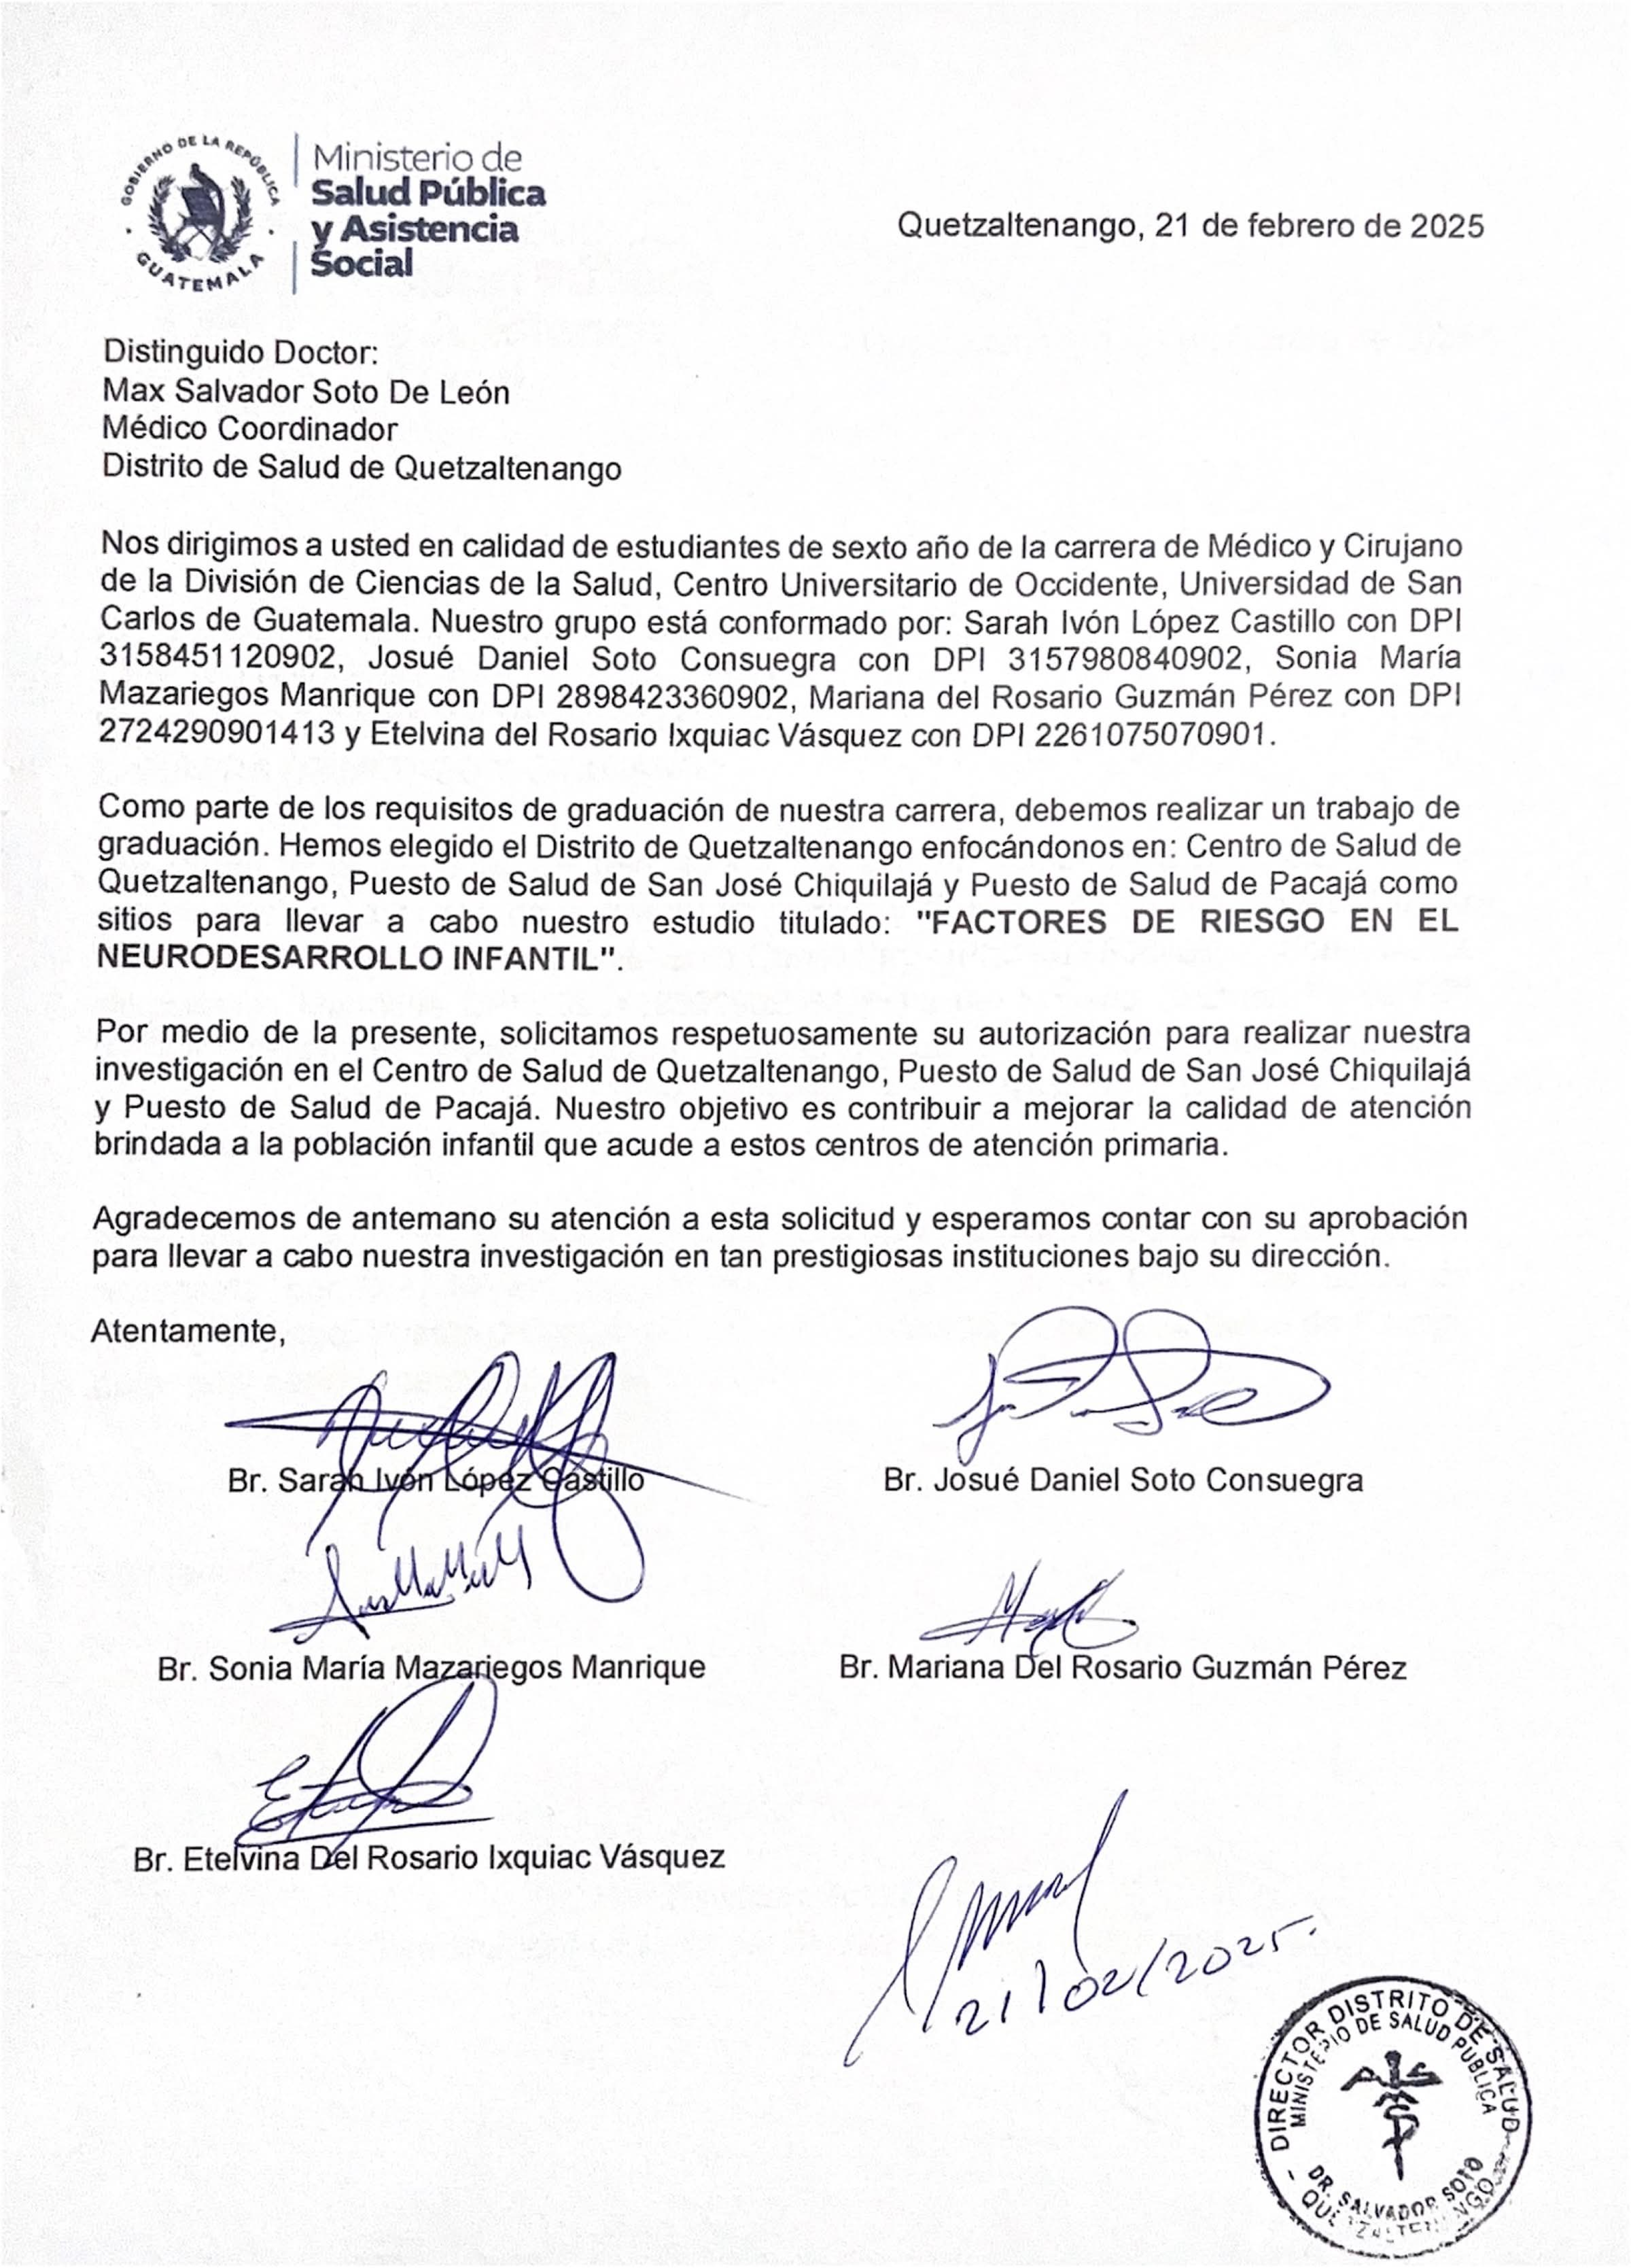
\includepdf[scale=0.9,pages=-,
  pagecommand={\thispagestyle{plain}\vspace*{0pt}\begin{center}\Large\bfseries Apéndice B: Permiso institucional\end{center}\vspace{1cm}}
]{extras/permiso.pdf}

\cleardoublepage
\stepcounter{chapter}
\phantomsection
\addcontentsline{toc}{chapter}{Apéndice C: Consentimiento informado}
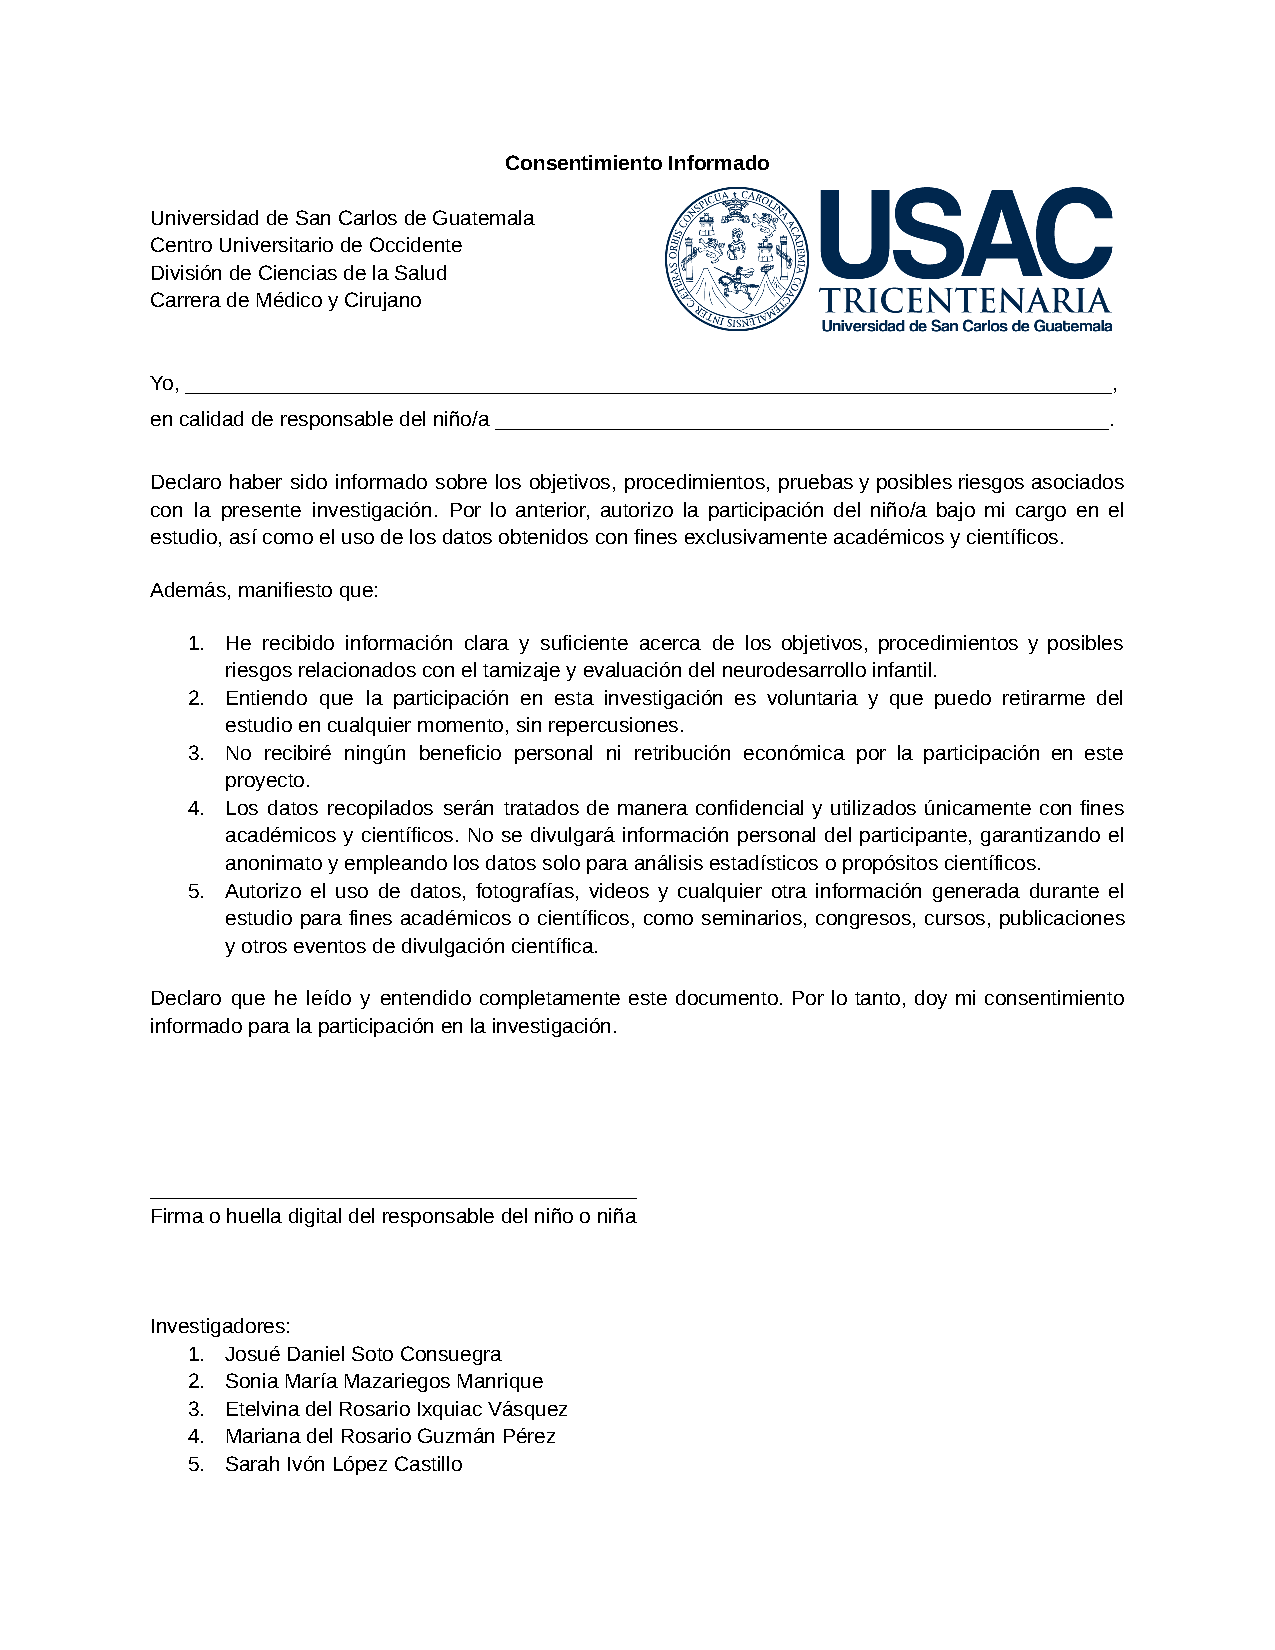
\includepdf[scale=0.9,pages=-,
  pagecommand={\thispagestyle{plain}\vspace*{0pt}\begin{center}\Large\bfseries Apéndice C: Consentimiento informado\end{center}\vspace{1cm}}
]{images/consentimiento.pdf}

\cleardoublepage
\stepcounter{chapter}
\phantomsection
\addcontentsline{toc}{chapter}{Apéndice D: Boleta de recolección de datos}
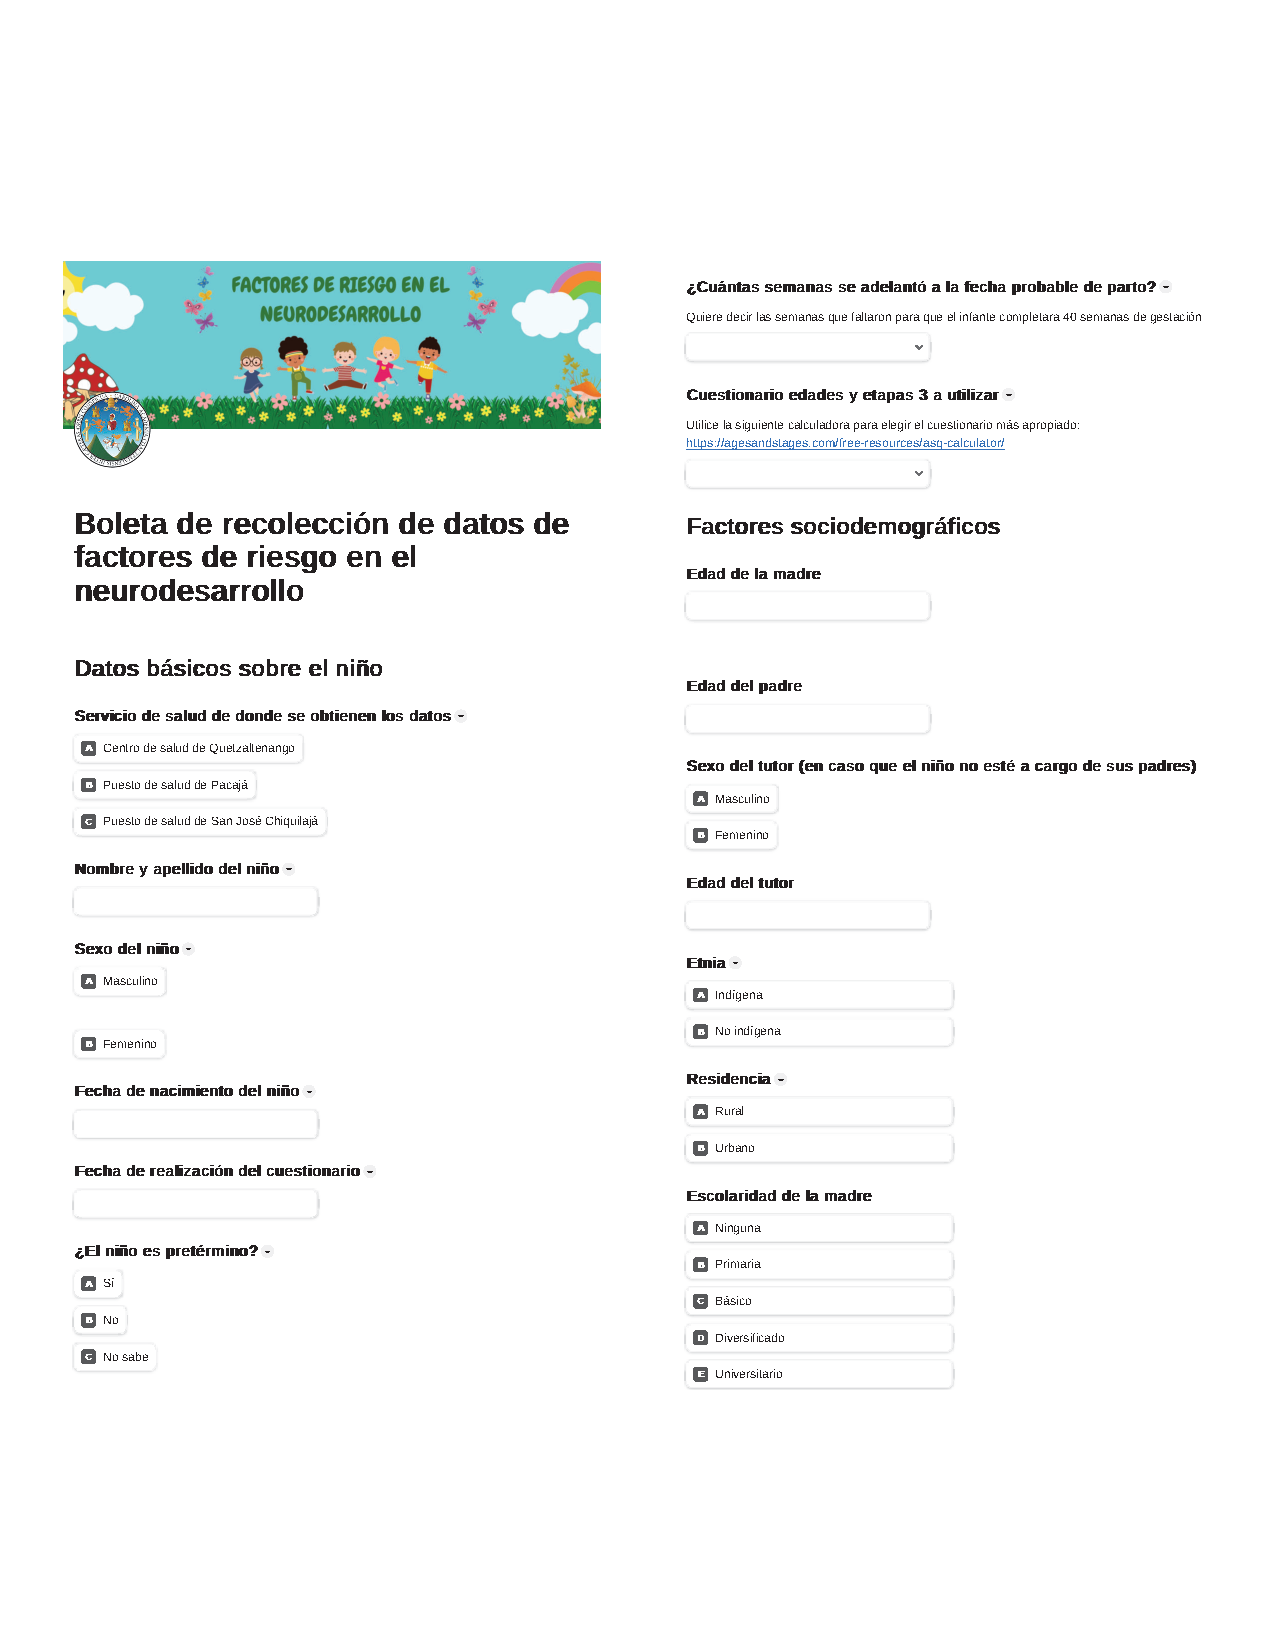
\includepdf[scale=0.85,pages=-,
  pagecommand={\thispagestyle{plain}\vspace*{0pt}\begin{center}\Large\bfseries Apéndice D: Boleta de recolección de datos\end{center}\vspace{1cm}}
]{images/boleta.pdf}

\cleardoublepage
\stepcounter{chapter}
\phantomsection
\addcontentsline{toc}{chapter}{Apéndice E: Ejemplo de Cuestionario Edades y Etapas 3}
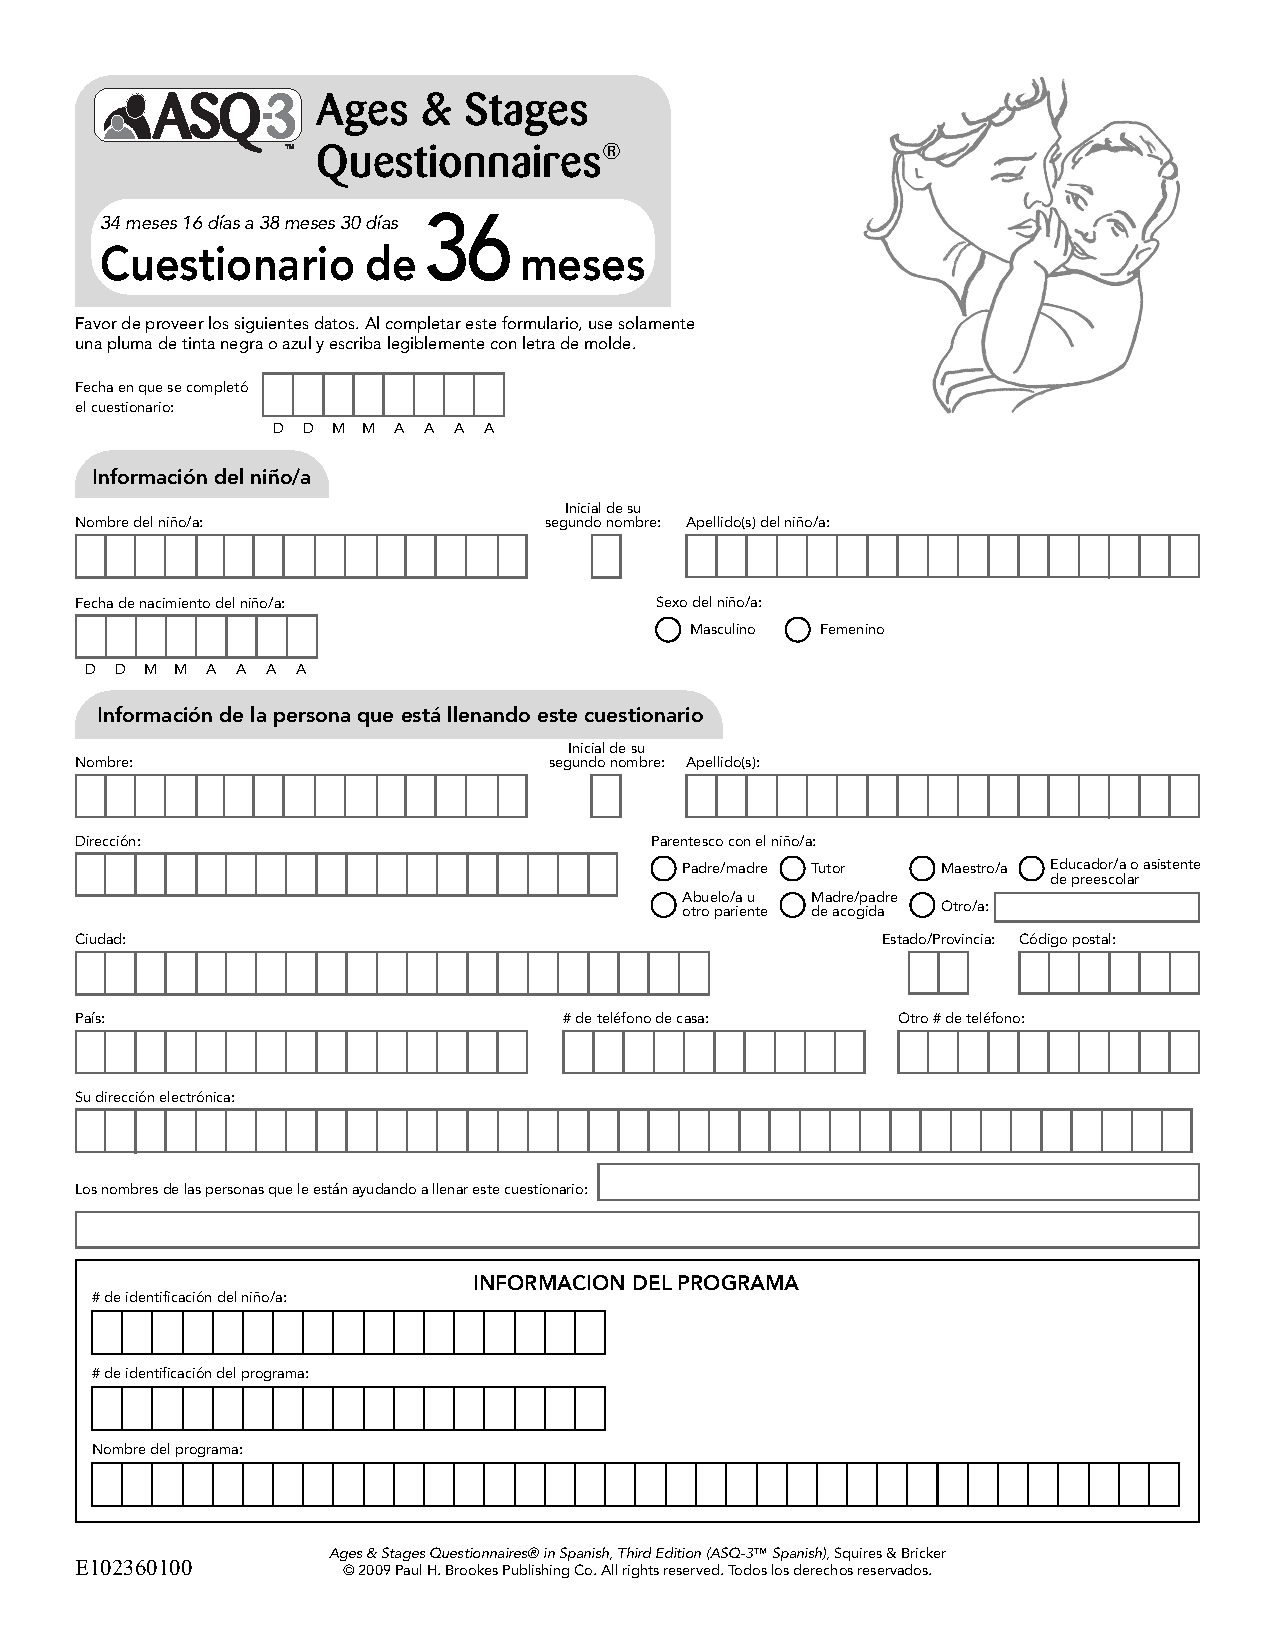
\includepdf[scale=0.80,pages=1-5,
  pagecommand={\thispagestyle{plain}\vspace*{0pt}\begin{center}\Large\bfseries Apéndice E: Ejemplo de Cuestionario Edades y Etapas 3\end{center}\vspace{1cm}}
]{images/36meses.pdf}

\cleardoublepage
\stepcounter{chapter}
\phantomsection
\addcontentsline{toc}{chapter}{Apéndice F: Resultados de análisis de porcentaje de plagio}
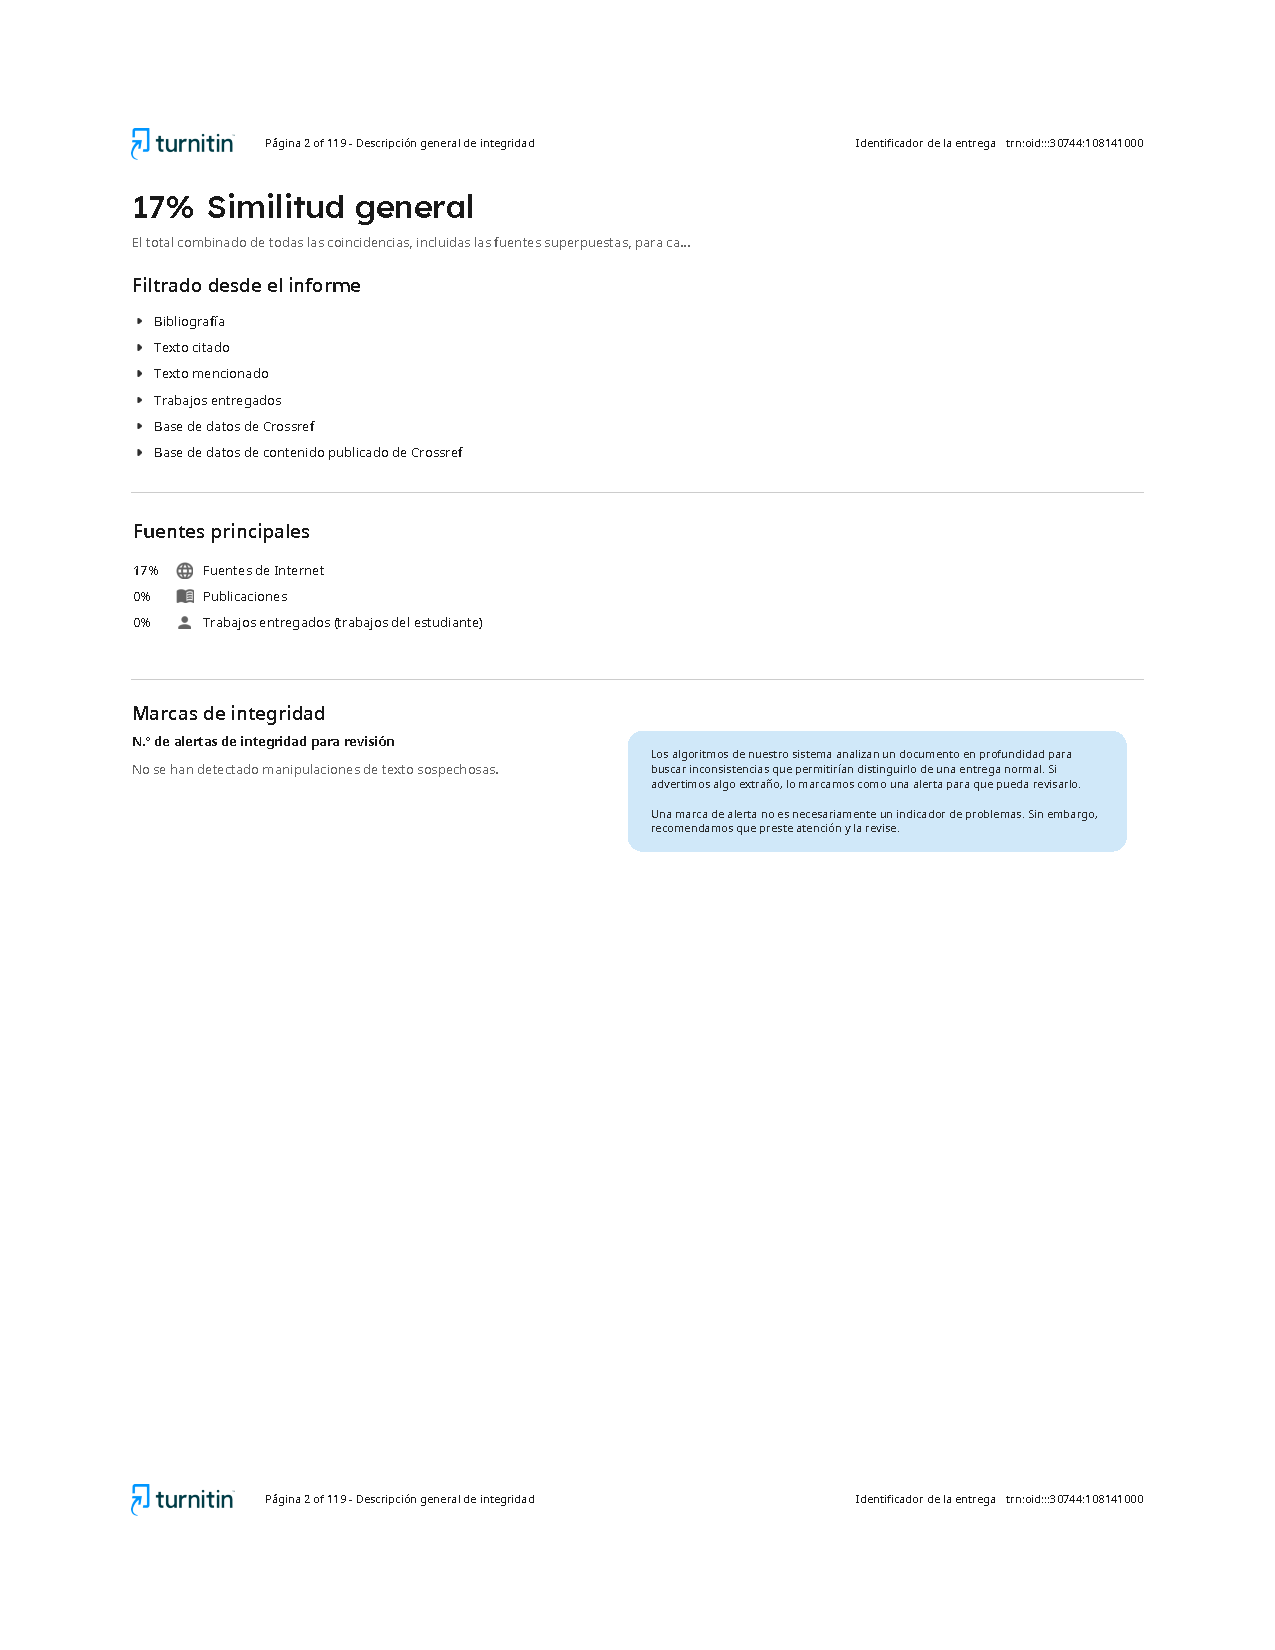
\includepdf[scale=0.80,
  pagecommand={\thispagestyle{plain}\vspace*{0pt}\begin{center}\Large\bfseries Apéndice F: Resultados de análisis de porcentaje de plagio\end{center}\vspace{1cm}}
]{extras/turnitin.pdf}

\chapter*{Permiso para Reproducción de los Contenidos de la Investigación}

Este trabajo está bajo una Licencia Creative Commons Atribución 4.0 Internacional.

\begin{center}

\includegraphics[width=0.2\textwidth]{images/cc-by.png}
\end{center}

Usted es libre de:
\begin{itemize}
    \item \textbf{Compartir} — copiar y redistribuir el material en cualquier medio o formato
    \item \textbf{Adaptar} — remezclar, transformar y construir a partir del material para cualquier propósito, incluso comercialmente
\end{itemize}

Bajo los siguientes términos:
\begin{itemize}
    \item \textbf{Atribución} — Usted debe dar crédito de manera adecuada, brindar un enlace a la licencia, e indicar si se han realizado cambios. Puede hacerlo en cualquier forma razonable, pero no de forma tal que sugiera que usted o su uso tienen el apoyo del licenciante.
    \item \textbf{Sin restricciones adicionales} — No puede aplicar términos legales ni medidas tecnológicas que restrinjan legalmente a otras personas hacer cualquier uso permitido por la licencia.
\end{itemize}

Avisos:
\begin{itemize}
    \item No tiene que cumplir con la licencia para elementos del material en el dominio público o cuando su uso esté permitido por una excepción o limitación aplicable.
    \item No se dan garantías. La licencia podría no darle todos los permisos que necesita para el uso que tenga previsto.
    \item Pueden existir derechos de terceros sobre algunos elementos como imágenes, gráficos u otros contenidos que requieran autorizaciones adicionales para su uso.
\end{itemize}

Para ver una copia de esta licencia, visite:\\ 
\url{http://creativecommons.org/licenses/by/4.0/deed.es}

\end{document}
